\documentclass{report}

\usepackage{hyperref}
\hypersetup{
	colorlinks=true,
	linkcolor=blue,
	filecolor=magenta,
	urlcolor=cyan,
}

\usepackage{amsthm, amsmath, amsfonts, mathrsfs, amssymb, bbm}
\usepackage[]{cancel}
\usepackage{cleveref}
\usepackage{graphicx,wrapfig}
\newtheorem{thm}{Theorem}[section]
\newtheorem{prop}[thm]{Proposition}
\newtheorem{coro}[thm]{Corollary}
\newtheorem{lem}[thm]{Lemma}
\theoremstyle{remark}
\newtheorem{rmk}{Remark}[chapter]
\theoremstyle{definition}
\newtheorem{defn}{Definition}[chapter]
\newtheorem{example}[defn]{Example}

\usepackage{biblatex}
\addbibresource{Bibliography.bib}

\newcommand{\diff}{\operatorname{d}}

\title{Existence and Uniqueness of Barycenter on Metric Space}
\author{Jianyu MA}
\date{\today}

\begin{document}
\maketitle

\begin{abstract}
	We can generalize physical concept of barycenter from Euclidean space to abstract metric space.
	Both existence and uniqueness of barycenter are not clear in advance.
	With this in mind, from abstract to concrete,
	we investigate these two properties of barycenters on general metric space,
	Wasserstein space over proper metric space and Wasserstein space over complete manifold.
	In the last case, a barycenter is a measure on manifold and we discuss its absolutely continuity.
	% Current working plan is:
	% \begin{itemize}
	% \item Verify example of non-uniqueness in relation of non-branching: four points by M.Bertrand
	% \item Hilbert manifold geometric properties
	% \item Counter examples of non-uniqueness and reasons
	% \item Familiar with measure theory of metric space
	% \item Study convex analysis
	% \item Paper review of \cite{KIM2017640}
	% \item Formulate a concise proof of main results in \cite{KIM2017640}
	% \item Measure theory on Riemannian manifold
	% \item Show that barycenter distance function is continuous.
	% \item Write final report
	% \item Discussion of uniqueness on metric space
	% \item More detailed analysis of differentiability of $(f_i / \lambda_i)^c$
	% \item Upper Lipschitz bound of exponential map
	% \item \textcolor{red}{Impossible:} Justify differentiating of barycenter identity
	% \item Consistency of barycenter on manifold, shrink nicely by barycenter formula.
	% \end{itemize}
\end{abstract}

\tableofcontents

%! TEX root = ../barycenter.tex
\chapter{Introduction and preparation}
\section{Definition of barycenter}
To begin with, recall in physics we define barycenter (or written as barycentre), i.e.,  center inertial mass, as a geometic point where we can image gravity acts at. In the case of a system of particles $\boldsymbol{P}_\nu$, $\nu = 1, \ldots , N$, each with mass $m_\nu$ that are located in space with coordinates $\boldsymbol{r}_\nu$, $\nu = 1, \ldots , N$, the coordinate of the center of mass $C$ satisfies condition:
\[
	\sum _{\nu=1}^{N} m_{\nu}\boldsymbol {r}_{\nu} -	\sum _{\nu=1}^{N}m_{\nu}\boldsymbol {r}_C = \sum _{\nu=1}^{N}m_{\nu}(\boldsymbol {r} _{\nu}-\boldsymbol {r}_C )=\boldsymbol {0}.
\]
Then set \( M := \sum _ { \nu = 1 } ^ { N } m _ { \nu } \), we should have
\[
	\boldsymbol { r } _ { C } = \left( \sum _ { \nu = 1 } ^ { N } m _ { \nu } \boldsymbol { r } _ { \nu } \right) / M .
\]
We can characterize barycenter as the unique solution of minimizing problem
\begin{equation}
	\label{barycenter_def}
	\boldsymbol{r}_C = \operatorname{arg} \min_{\boldsymbol{r}} \sum_{\nu= 1}^N \frac{m_\nu}{M} \Vert \boldsymbol{r}_{\nu} - \boldsymbol{r}\Vert^2
\end{equation}
as norm is calculated as inner product on Eculidean space.

To generalize \ref{barycenter_def}, there are two core concepts to keep: metric distance and measure integral.

\section{Geometry and probability background}
We should introduce necessary concepts and recall classic results to help our discussion; for the sake of instruction, we present some classic proofs.
\subsection{Metric geometry}
\subsection{Measure theory}

Let \( X \) be a metric space and \( \mathscr { M } ( X ) \) the space of all measures defined on \( \mathscr { B } _ { X } . \) An element \( \mu \in \mathscr { H } ( X ) \) is a nonnegative, countably additive set function defined on \( \mathscr { B } _ { X } \) with the property \( \mu ( X ) = 1 . \quad C ( X ) \) stands for the space of all bounded real valued continuous functions on \( X \).  We shall now topologize the space \( \mathscr { M } ( X ) \) by defining a base of open neighborhoods for any point \( \mu . \) Consider the family of sets of the form
\( V _ { \mu } \left( f _ { 1 } , f _ { 2 } , \ldots , f _ { k } ; \varepsilon _ { 1 } , \ldots , \varepsilon _ { k } \right) \)
\[ \left\{\nu \in \mathscr { M } ( X ) \, \mid  \left| \int f _ { i } d v - \int f _ { i } d \mu \right| < \varepsilon _ { i } , \quad i = 1,2 , \ldots , k \right\} \]

where \( f _ { 1 } , f _ { 2 } , \ldots , f _ { k } \) are elements from \( C ( X ) \) and \( \varepsilon _ { 1 } , \varepsilon _ { 2 } , \ldots , \varepsilon _ { k } , \) are positive numbers. It is easy to verify that the family of sets obtained by varying \( k , f _ { 1 } , f _ { 2 } , \ldots , f _ { k } , \varepsilon _ { 1 } , \ldots , \varepsilon _ { k } \) satisfies the axioms of a basis for a topology.

\begin{defn}
	We shall refer to this as the weak topology  in \( \mathscr { M } ( X ) \).
\end{defn}

It is then clear that a net \( \left\{ \mu _ { \alpha } \right\} \) of measures converges in the weak topology to a measure \( \mu \) if and only if \( \int f d \mu _ { \alpha } \rightarrow \int f d \mu \) for every \( f \in C ( X ) . \) In such a case we shall say that \( \mu _ { \alpha } \) converges "weakly" to \( \mu \) or \( \mu _ { \alpha } \Rightarrow \mu \) in symbols. Unless otherwise stated, \( \mathscr { M } ( X ) \) will always be considered as a topological space with the weak topology.

We shall first recall a theorem which yields several useful equivalent definitions of the weak topology.

\begin{thm}
	Let \( \mu _ { \alpha } \) be a net in \( \mathscr { M } ( X ) . \) Then the following statements are equivalent:
	\begin{itemize}
		\label{weak_convergence_thm}
		\item \( \mu _ { \alpha } \Rightarrow \mu \)
		\item \( \lim _ { \alpha } \int g d \mu _ { \alpha } = \int g d \mu \) for all \( g \in U ( X ) \) where \( U ( X ) \) is the space of all bounded real valued uniformly continuous functions;
		\item \( \overline { \lim } _ { \alpha } \mu _ { \alpha } ( C ) \leqslant \mu ( C ) \) for every closed set \( C \)
		\item \( \lim _ { \alpha } \mu _ { \alpha } ( G ) \geqslant \mu ( G ) \) for every open set \( G \)
		\item \( \lim _ { \alpha } \mu _ { \alpha } ( A ) = \mu ( A ) \) for every Borel set \( A \) whose boundary has \( \mu \) -measure \( 0 . \)
	\end{itemize}
\end{thm}

For each point \( x \in X \) we shall denote by \( p _ { x } \) the measure degenerate at the point \( x \). Denote \( D = \left\{ p _ { x }: x \in X \right\} \).

\begin{lem}
	\label{dirac_measure_weak_homeomeorphic}
	\( X \) is homeomorphic to the (topological) subset $D$.
\end{lem}

\begin{proof}
	For any point \( x \) and \( g \in C ( X ) , \) we have \( \int g d p _ { x } = g ( x ) \). If \( x _ { \alpha } \rightarrow x _ { 0 } \) then \( g \left( x _ { \alpha } \right) \rightarrow g \left( x _ { 0 } \right) . \) Hence \( p _ { x _ { \alpha } } \Rightarrow p _ { x _ { 0 } } \). Conversely, let \( p _ { x _ { \alpha } } \Rightarrow p _ { x _ { 0 } } \) If \( x _ { \alpha } \) does not converge to \( x _ { 0 } \), there is an open set \( G \) and a subnet \( \left\{ x _ { \beta } \right\} \) such that \( x _ { 0 } \in G \) and \( x _ { \beta } \in X - G \) for all \( \beta . \) Let \( g \) be a continuous function such that \( 0 \leqslant g \leqslant 1 , g \left( x _ { 0 } \right) = 0 \) and \( g ( x ) = 1 \) for \( x \in X - G \). Then \( \int g d p _ { x _ { \beta } } = 1 , \) while \( \int g d p _ { x _ { 0 } } = 0 . \) This is a contradiction. This completes the proof.
\end{proof}

\begin{lem}
	\( D \) is a sequentially closed subset of \( \mathscr { M } ( X ) \).
\end{lem}

\begin{proof}
	Let \( \left\{ x _ { n } \right\} \) be a sequence of points in \( X \) such that \( p _ { x _ { n } } \Rightarrow q \) Suppose \( \left\{ x _ { n } \right\} \) does not have any convergent subsequence. Then the set \( S = \left\{ x _ { 1 } , x _ { 2 } , \ldots \right\} \) is closed and thus is any subset \( C \) of \( S . \) Since \( p _ { x _ { n } } \Rightarrow q \) we have by Theorem \ref{weak_convergence_thm}, \( q ( C ) \geqslant \overline { \lim } p _ { x _ { n } } ( C ) \) for \( C \subseteq S \). It follows that for every infinite subset \( S _ { 1 } \subseteq S , q \left( S _ { 1 } \right) = 1 \). This is a contradiction since \( q \) is a measure.

	Thus there is a subsequence \( \left\{ x _ { n _ { k } } \right\} , x _ { n _ { k } } \rightarrow x . \) By Lemma \ref{dirac_measure_weak_homeomeorphic}, \( q = p _ { x } \). Hence \( D \) is sequentially closed.
\end{proof}


\begin{thm}
	\label{finite_support_approximation}
	Let \( X \) be a separable metric space and \( E \subseteq X \) dense in \( X  \). Then the set of all measures whose supports are finite subsets of \( E \) is dense in \( \mathscr{ M } ( X ) \), the set of all Borel probability measures on $X$.
\end{thm}

\begin{proof}
	This proof is copy from Theorem 6.3 in \cite{parthasarathy2005probability}.

	It is obviously enough to prove that the set of all measures whose supports are finite subsets of \( X \) is dense in \( \mathscr { M } ( X ) . \) Let us denote the class of such measures by \( \mathscr { F } ( X ) . \) It is clear that any measure concentrated in a countable subset of \( X \) is a weak limit of measures from \( \mathscr { F } ( X ) . \) Thus it is sufficient to prove that any measure is a weak limit of measures vanishing outside countable subsets of \( X \).

	Choose and fix \( \mu \in \mathscr { M } ( X ) \). Since \( X \) is separable we can, for each integer \( n , \) write \( X \) as \( \bigcup _ { j } A _ { n j } , A _ { n j } \cap A _ { n k } = \phi \) if \( j \neq k , A _ { n j } \in \mathscr { B } _ { X } \) for all \( n \) and \( j \) and the diameter of \( A _ { n j } \) is \( \leq 1 / n \) for all \( j \). Let \( x _ { n j } \in A _ { n j } \) be arbitrary. Let \( \mu _ { n } \) be the measure with masses \( \mu \left( A _ { n j } \right) \) at the points \( x _ { n j } , \) respectively. Let $g$ be an arbitrary uniformly continuous (we can even assume Lipschitz continous here) bounded function, and let \[ \alpha _ { n j } = \inf _ { x \in A _ { n j } } g ( x ) , \quad \beta _ { n j } = \sup _ { x \in A _ { n j } } g ( x ) \]
	Since \( g \) is uniformly continuous and since the diameter of \( A _ { n j } \rightarrow 0 \) as \( n \rightarrow \infty \) uniformly in \( j , \sup _ { j } \left( \beta _ { n j } - \alpha _ { n j } \right) \rightarrow 0 \) as \( n \rightarrow \infty \). Now
	\begin{align*}
		\left| \int g d \mu _ { n } - \int g d \mu \right| & = \left| \sum \int _ { A _ { n j } } \left( g - g \left( x _ { n j } \right) \right) d \mu \right|     \\
		                                                   & \leq \sup_{j} \left( \beta _ { n j } - \alpha _ { n j } \right) \xrightarrow{ n \rightarrow \infty} 0.
	\end{align*}
\end{proof}

\begin{thm}[Prokhorov's theorem]
	If \( \mathcal { X } \) is a Polish space, then a set \( \mathcal { P } \subset P ( \mathcal { X } ) \) is precompact for the weak topology if and only if it is tight, i.e. for any \( \varepsilon > 0 \) there is a compact set \( K _ { \varepsilon } \) such that \( \mu \left[ \mathcal { X } \backslash K _ { \varepsilon } \right] \leq \varepsilon \) for all \( \mu \in \mathcal { P } \).
\end{thm}

\section{Optimal transportation}
We start with a basic definition in probability theory.

\begin{defn}[Coupling]
	Let \( ( \mathcal { X } , \mu ) \) and \( ( \mathcal { Y } , \nu ) \) be two probability spaces. Coupling \( \mu \) and \( \nu \) means constructing two random variables \( X \) and \( Y \) on some probability space \( ( \Omega , \mathbb { P } ) , \) such that law \( ( X ) = \mu \), law \( ( Y ) = \nu . \) The couple \( ( X , Y ) \) is called a coupling of \( ( \mu , \nu ) . \) By abuse of language, the law of \( ( X , Y ) \) is also called a coupling of \( ( \mu , \nu ) \).
\end{defn}

If \( \mu \) and \( \nu \) are the only laws in the problem, then without loss of generality one may choose \( \Omega = \mathcal { X } \times \mathcal { Y } . \) In a more measure-theoretical formulation, coupling \( \mu \) and \( \nu \) means constructing a measure \( \pi \) on \( \mathcal { X } \times \mathcal { Y } \) such that \( \pi \) admits \( \mu \) and \( \nu \) as marginals on \( \mathcal { X } \) and \( \mathcal { Y } \) respectively.


We then define the optimal coupling or optimal transport. Here one introduces a cost function \( c ( x , y ) \) on \( \mathcal { X } \times \mathcal { Y } , \) that can be interpreted as the work needed to move one unit of mass from location \( x \) to location \( y . \) Then one considers the Monge-Kantorovich minimization problem
\[
	\operatorname{inf}  \mathbb { E } c ( X , Y )
\]
where the pair \( ( X , Y ) \) runs over all possible couplings of \( ( \mu , \nu ) ; \) or equivalently, in terms of measures,
\[ \inf \int _ { \mathcal { X } \times \mathcal { Y } } c ( x , y ) d \pi ( x , y ) \]
where the infimum runs over all joint probability measures \( \pi \) on \( \mathcal { X } \times \mathcal { Y } \) with marginals \( \mu \) and \( \nu . \) Such joint measures are called trans- ference plans (or transport plans, or transportation plans); those achieving the infimum are called optimal transference plans.

The first good thing about optimal couplings is that they exist:
\begin{thm}[Existence of an optimal coupling]
	Let \( ( \mathcal { X } , \mu ) \) and \( ( \mathcal { Y } , \nu ) \) be two Polish probability spaces; let \( a: \mathcal { X } \rightarrow \mathbb { R } \cup \{ - \infty \} \) and \( b: \mathcal { Y } \rightarrow \mathbb { R } \cup \{ - \infty \} \) be two upper semicontinuous functions such that \( a \in L ^ { 1 } ( \mu ) , b \in L ^ { 1 } ( \nu ) . \) Let \( c: \mathcal { X } \times \mathcal { Y } \rightarrow \mathbb { R } \cup \{ + \infty \} \) be a lower semicontinuous cost function, such that \( c ( x , y ) \geq a ( x ) + b ( y ) \) for all \( x , y . \) Then there is a coupling of \( ( \mu , \nu ) \) which minimizes the total cost \( \mathbb { E } c ( X , Y ) \) among all possible couplings \( ( X , Y ) \).
\end{thm}
The proof relies on basic variational arguments involving the topology of weak convergence (i.e. imposed by bounded continuous test functions). There are two key properties to check: (a) lower semicontinuity, (b) compactness. These issues are taken care of respectively in two lemmas below.

\begin{lem}[Lower semicontinuity of the cost functional]
	\label{lower_semicontinuity_of_the_cost_functional}
	Let \( \mathcal { X } \) and \( \mathcal { Y } \) be two Polish spaces, and \( c: \mathcal { X } \times \mathcal { Y } \rightarrow \mathbb { R } \cup \{ + \infty \} \) a lower semicontinuous cost function. Let \( h: \mathcal { X } \times \mathcal { Y } \rightarrow \mathbb { R } \cup \{ - \infty \} \) be an upper semicontinuous function such that \( c \geq h . \) Let \( \left( \pi _ { k } \right) _ { k \in \mathbb { N } } \) be a sequence of
	probability measures on \( \mathcal { X } \times \mathcal { Y } , \) converging weakly to some \( \pi \in P ( \mathcal { X } \times \mathcal { Y } ) \), in such a way that \( h \in L ^ { 1 } \left( \pi _ { k } \right) , h \in L ^ { 1 } ( \pi ) , \) and
	\[ \int _ { \mathcal { X } \times \mathcal { Y } } h d \pi _ { k } \underset { k \rightarrow \infty } { \longrightarrow } \int _ { \mathcal { X } \times \mathcal { Y } } h d \pi \]
	\[ \int _ { \mathcal { X } \times \mathcal { Y } } c d \pi \leq \liminf _ { k \rightarrow \infty } \int _ { \mathcal { X } \times \mathcal { Y } } c d \pi _ { k } \]
	In particular, if \( c \) is nonnegative, then \( F: \pi \rightarrow \int c d \pi \) is lower semicontinuous on \( P ( \mathcal { X } \times \mathcal { Y } ) , \) equipped with the topology of weak convergence.
\end{lem}

\begin{proof}
 Replacing \( c \) by \( c - h , \) we may assume that \( c \) is a nonnegative lower semicontinuous function. Then \( c \) can be written as the pointwise limit of a nondecreasing family \( \left( c _ { \ell } \right) _ { \ell \in \mathbb { N } } \) of continuous real-valued functions. By monotone convergence,
	\[ \int c d \pi = \lim _ { \ell \rightarrow \infty } \int c _ { \ell } d \pi = \lim _ { \ell \rightarrow \infty } \lim _ { k \rightarrow \infty } \int c _ { \ell } d \pi _ { k } \leq \liminf _ { k \rightarrow \infty } \int c d \pi _ { k } \]
\end{proof}
\begin{lem}[Tightness of transference plans]
	Let \( \mathcal { X } \) and \( \mathcal { Y } \) be two Polish spaces. Let \( \mathcal { P } \subset P ( \mathcal { X } ) \) and \( \mathcal { Q } \subset P ( \mathcal { Y } ) \) be tight subsets of \( P ( \mathcal { X } ) \) and \( P ( \mathcal { Y } ) \) respectively. Then the set \( \Pi ( \mathcal { P } , \mathcal { Q } ) \) of all transference plans whose marginals lie in \( \mathcal { P } \) and \( \mathcal { Q } \) respectively, is itself tight in \( P ( \mathcal { X } \times \mathcal { Y } ) \).
\end{lem}

\begin{proof}
 Let \( \mu \in \mathcal { P } , \nu \in \mathcal { Q } , \) and \( \pi \in \Pi ( \mu , \nu ) . \) By assump- tion, for any \( \varepsilon > 0 \) there is a compact set \( K _ { \varepsilon } \subset \mathcal { X } , \) independent of the choice of \( \mu \) in \( \mathcal { P } \), such that \( \mu \left[ \mathcal { X } \backslash K _ { \varepsilon } \right] \leq \varepsilon ; \) and similarly there is a compact set \( L _ { \varepsilon } \subset \mathcal { Y } , \) independent of the choice of \( \nu \) in \( \mathcal { Q } , \) such that \( \nu \left[ \mathcal { Y } \backslash L _ { \varepsilon } \right] \leq \varepsilon . \) Then for any coupling \( ( X , Y ) \) of \( ( \mu , \nu ) \)
	\[ \mathbb { P } \left[ ( X , Y ) \notin K _ { \varepsilon } \times L _ { \varepsilon } \right] \leq \mathbb { P } \left[ X \notin K _ { \varepsilon } \right] + \mathbb { P } \left[ Y \notin L _ { \varepsilon } \right] \leq 2 \varepsilon. \]

	The desired result follows since this bound is independent of the coupling, and \( K _ { \varepsilon } \times L _ { \varepsilon } \) is compact in \( \mathcal { X } \times \mathcal { Y }  \).
\end{proof}

By passing to the limit in the equation for marginals, we see that \( \Pi ( \mu , \nu ) \) is closed, so it is in fact compact. Then let \( \left( \pi _ { k } \right) _ { k \in \mathbb { N } } \) be a sequence of probability measures on \( \mathcal { X } \times \mathcal { Y } \), such that \( \int c d \pi _ { k } \) converges to the infimum transport cost. Extracting a subsequence if necessary, we may assume that \( \pi _ { k } \) converges to some \( \pi \in \Pi ( \mu , \nu ) . \) The function \( h: ( x , y ) \longmapsto a ( x ) + b ( y ) \) lies in \( L ^ { 1 } \left( \pi _ { k } \right) \) and in \( L ^ { 1 } ( \pi ) \), and \( c \geq h \) by assumption; moreover, \( \int h d \pi _ { k } = \int h d \pi = \) \( \int a d \mu + \int b d \nu \); so Lemma 4.3 implies
\[ \int c d \pi \leq \liminf _ { k \rightarrow \infty } \int c d \pi _ { k }. \]

Thus $\pi$ is minimizing.
\subsection{Wasserstein space}

\begin{defn}[Wasserstein distances]
	\label{Wasserstein_distance}
	Let  \(( \mathcal { X } , d ) \) be a Polish metric space, and let \( p \in [ 1 , \infty ) . \) For any two probability measures \( \mu , \nu \) on \( \mathcal { X } , \) the Wasserstein distance of order \( p \) between \( \mu \) and \( \nu \) is defined by the formula
	\begin{align*}
		W _ { p } ( \mu , \nu ) & = \left( \inf _ { \pi \in \Pi ( \mu , \nu ) } \int _ { \mathcal { X } } d ( x , y ) ^ { p } d \pi ( x , y ) \right) ^ { 1 / p }                                                      \\
		                        & = \inf \left\{ \left[ \mathbb { E } d ( X , Y ) ^ { p } \right] ^ { \frac { 1 } { p } } , \quad \operatorname { law } ( X ) = \mu , \quad \operatorname { law } ( Y ) = \nu \right\}
	\end{align*}
\end{defn}

\begin{lem}
	\label{lower_semicontinous_Wasserstein_distance}
	Wasserstein distance is lower semi-continous with respect to weakly convergence of measures on $P(\mathscr{X})$.
\end{lem}

\begin{proof}
	This is a direct consequence of lower semicontinuity of the cost functional, see lemma \ref{lower_semicontinuity_of_the_cost_functional}.
\end{proof}

\begin{defn}[Wasserstein space]
	\label{Wasserstein_space}
	With the same conventions as in Definition \ref{Wasserstein_distance} , the Wasserstein space of order \( p \) is defined as
	\[
		P _ { p } ( \mathcal { X } ): = \left\{ \mu \in P ( \mathcal { X } ) ; \quad \int _ { \mathcal { X } } d \left( x _ { 0 } , x \right) ^ { p } \mu ( d x ) < + \infty \right\}
	\]
	where \( x _ { 0 } \in \mathcal { X } \) is arbitrary. This space does not depend on the choice of the point \( x _ { 0 } \). Then \( W _ { p } \) defines a (finite) distance on \( P _ { p } ( \mathcal { X } ) \).
\end{defn}

\begin{defn}[Weak convergence in \( P _ { p } \) ]
	Let \( ( \mathcal { X } , d ) \) be a Polish space, and \( p \in [ 1 , \infty ) \). Let \( \left( \mu _ { k } \right) _ { k \in \mathbb { N } } \) be a sequence of probability measures in \( P _ { p } ( X ) \) and let \( \mu \) be another element of \( P _ { p } ( \mathcal { X } ) . \) Then \( \left( \mu _ { k } \right) \) is said to converge weakly in \( P _ { p } ( \mathcal { X } ) \) if any one of the following equivalent properties is satisfied for some (and then any) \( x _ { 0 } \in \mathcal { X }: \)
	\begin{enumerate}
		\item \( \mu _ { k } \longrightarrow \mu \) and \( \int d \left( x _ { 0 } , x \right) ^ { p } d \mu _ { k } ( x ) \longrightarrow \int d \left( x _ { 0 } , x \right) ^ { p } d \mu ( x ) \)
		\item \( \mu _ { k } \longrightarrow \mu \) and \( \limsup _ { k \rightarrow \infty } \int d \left( x _ { 0 } , x \right) ^ { p } d \mu _ { k } ( x ) \leq \int d \left( x _ { 0 } , x \right) ^ { p } d \mu ( x ) \)
		\item \( \mu _ { k } \longrightarrow \mu \) and \( \lim _ { R \rightarrow \infty } \limsup _ { k \rightarrow \infty } \int _ { d \left( x _ { 0 } , x \right) \geq R } d \left( x _ { 0 } , x \right) ^ { p } d \mu _ { k } ( x ) = 0 \)
		\item For all continuous functions \( \varphi \) with \( | \varphi ( x ) | \leq C \left( 1 + d \left( x _ { 0 } , x \right) ^ { p } \right) \)
		      \( C \in \mathbb { R } \), one has
		      \[ \int \varphi ( x ) d \mu _ { k } ( x ) \longrightarrow \int \varphi ( x ) d \mu ( x ) \]
	\end{enumerate}
\end{defn}

\begin{thm}[$W _ { p }$  metrizes \( P _ { p } \)]
	Let \( ( \mathcal { X } , d ) \) be a Polish space, and \( p \in [ 1 , \infty ) ; \) then the Wasserstein distance \( W _ { p } \) metrizes the weak convergence in \( P _ { p } ( \mathcal { X } ) . \) In other words, if \( \left( \mu _ { k } \right) _ { k \in \mathbb { N } } \) is a sequence of measures in \( P _ { p } ( \mathcal { X } ) \) and \( \mu \) is another measure in \( P ( \mathcal { X } ) , \) then the statements
	\[ \mu _ { k } \text { converges weakly in } P _ { p } ( \mathcal { X } ) \text { to } \mu \]
	and
	\[ W _ { p } \left( \mu _ { k } , \mu \right) \longrightarrow 0 \]
	are equivalent.
\end{thm}

For topology property of Wasserstein space, we refer to Theorem 6.18 in \cite{villani2008optimal}. This result is also a nature extension of general finite support measure approximation theorem \ref{finite_support_approximation}.
\begin{thm}[Toplogy of Wasserstein space]
	\label{topology_Wasserstein}
	Let \( \mathcal { X } \) be a complete separable metric space and \( p \in [ 1 , \infty ) \). Then the Wasserstein space \( P _ { p } ( \mathcal { X } ) , \) metrized by the Wasserstein distance \( W _ { p } , \) is also a complete separable metric space. In short: The Wasserstein space over a Polish space is itself a Polish space. Moreover, any probability measure can be approximated by a sequence of probability measures with finite support.
\end{thm}

\begin{thm}[Displacement interpolation as geodesics]
	\label{geodesic_Wasserstein_space}
	Let \( ( \mathcal { X } , d ) \) be a complete separable, locally compact length space. Let \( p > 1 \) and let \( P _ { p } ( \mathcal { X } ) \) be the space of probability measures on \( \mathcal { X } \) with finite moment of order \( p , \) metrized by the Wasserstein distance \( W _ { p } . \) Then, given any two \( \mu _ { 0 } , \mu _ { 1 } \in P _ { p } ( \mathcal { X } ) , \) and a continuous curve \( \left( \mu _ { t } \right) _ { 0 \leq t \leq 1 } , \) valued in \( P ( \mathcal { X } ) , \) the following properties are equivalent:
	\begin{enumerate}
		\item \( \mu _ { t } \) is the law of \(\gamma _ { t } \) where \( \gamma \) is a random (minimizing, constantspeed) geodesic such that \( \left( \gamma _ { 0 } , \gamma _ { 1 } \right) \) is an optimal coupling;
		\item \( \left( \mu _ { t } \right) _ { 0 \leq t \leq 1 } \) is a geodesic curve in the space \( P _ { p } ( \mathcal { X } ) \)
	\end{enumerate}
	Moreover, if \( \mu _ { 0 } \) and \( \mu _ { 1 } \) are given, there exists at least one such curve.
	More generally, if \( \mathcal { K } _ { 0 } \subset P _ { p } ( \mathcal { X } ) \) and \( \mathcal { K } _ { 1 } \subset \operatorname { P } _ { p } ( \mathcal { X } ) \) are compact subsets of
	\( P ( \mathcal { X } ) , \) then the set of geodesic curves \( \left( \mu _ { t } \right) _ { 0 < t < 1 } \) such that \( \mu _ { 0 } \in \mathcal { K } _ { 0 } \) and
	\( \mu _ { 1 } \in \mathcal { K } _ { 1 } \) is compact and nonempty; and also the set of dynamical opti-
	mal transference plans \( \Pi \) with \( \left( e _ { 0 } \right) _ { \# } \Pi \in \mathcal { K } _ { 0 } , \left( e _ { 1 } \right) _ { \# } \Pi \in \mathcal { K } _ { 1 } \) is compact
	and nonempty.
\end{thm}

%! TEX root = ../barycenter.tex
\chapter{Barycenter in Metric space}
\label{chapter:metric_space}
\section{Existence for proper space}

A metric space is proper if every bounded closed set is compact.
A proper (metric) space is complete and separable,
because we can write a proper metric space as a countable union of compact closed balls.
This assumption on compactness ensures the existence of barycenter.

\begin{prop}
	\label{lem:existence_proper_space}
	If \( ( E , d ) \) is a proper metric space, then any \( \mu \in \mathcal{W}_ { 2 } ( E ) \) has a barycenter.
\end{prop}

\begin{proof}
	Fix \( z _ { 0 } \in E \) and take \( r > 1 \) large enough to satisfy
	\[ \mu \left( B \left( z _ { 0 } , r \right) \right) \geq \frac { 1 } { 2 } , \quad \int _ { E \backslash B \left( z _ { 0 } , r \right) } d \left( z _ { 0 } , y \right) ^ { 2 } \diff \mu ( y ) \leq 1 \]
	Then we have
	\[ \int _ { E } d \left( z _ { 0 } , y \right) ^ { 2 } \diff \mu ( y ) \leq r ^ { 2 } \cdot \mu \left( B \left( z _ { 0 } , r \right) \right) + 1 \leq r ^ { 2 } + 1 \]
	while for every \( x \in E \backslash B \left( z _ { 0 } , 3 r \right) \)
	\[ \int _ { E } d ( x , y ) ^ { 2 } \diff \mu ( y ) \geq \int _ { B \left( z _ { 0 } , r \right) } d ( x , y ) ^ { 2 } \diff \mu ( y ) > ( 2 r ) ^ { 2 } \cdot \mu \left( B \left( z _ { 0 } , r \right) \right) \geq 2 r ^ { 2 } \]
	holds.
	Therefore, it is sufficient to consider the infimum of
	\[ x \longmapsto \int _ { E } d ( x , y ) ^ { 2 } \diff \mu ( y ) \]
	only for \( x \in B \left( z _ { 0 } , 3 r \right) , \) and it is achieved at some point due to the compactness of the closure of \( B \left( z _ { 0 } , 3 r \right) . \)
\end{proof}

Here is a simple example that shows lack of properness
violates the existence of barycenter given by \cite[Example 3.1 (a)]{ohta2012barycenters}.

\begin{example}
	\label{example:ellipsoid_subspace}
	Let \( E \) be the infinite dimensional ellipsoid of axes of lengths \( c _ { n } = ( n + 1 ) / 2 n \) with \( n \in \mathbb { N } , \) namely
	\[
		E = \left\{ \left( x _ { 1 } , x _ { 2 } , \ldots \right) \in \ell^2 | \sum _ { n \in \mathbb { N }^* } \frac { x _ { n } ^ { 2 } } { c _ { n } ^ { 2 } } = 1 \right\}
	\]

	Then \( E \) is complete as a closed subspace of Hilbert space $\ell^2,$
	but measure $\mu = \frac{1}{2}\delta _ { ( 1,0,0 , \ldots ) } + \frac{1}{2} \delta _ { ( - 1,0,0 , \ldots ) } $  has no barycenter in \( E \).
\end{example}

\begin{proof}
	$E$ is closed subspace of Hilbert space $\ell^2$ since $ 1 / 2 \leq c_{n} \leq 1$.
	Linear Hilbert structure enables us to calculate distance through inner product.
	Pick $ x \in E$ and set $ e=(1,0,0\ldots)$, by definition,
	\begin{align*}
		\int_{E} d(x, \cdot)^2 \diff \mu & = \frac{d(x,e)^2+d(x,-e)^2 }{2}                         \\
		                                 & =\frac{\| x - e \|^2 + \| x + e \|^2}{2} =\| x \|^2 + 1
	\end{align*}

	So a barycenter $z$ of $\mu$ in $E$ should minimize its length $\| z \|$,
	but it is impossible in this space.
	Assume now vector $z \in E$ attains minimal length.
	Consider first $n$ coordinate components of $z$,
	there could not exist any non-zero components except the last one, i.e., $z_i =0$ for $i<n$.
	Otherwise, we can keep coordinate components $z_j$ for $j>n$, which are out of consideration, unchanged but vanish first $n-1$ coordinate components to get a strictly shorter vector in $E$.
	This indicates that no such barycenter $z$ could exist in $E$.
\end{proof}

\begin{rmk}
	$E$ is not locally compact thus not a proper space.
	Indeed, consider the sequence with only one non-zero coordinate component, it has no converging subsequence.
\end{rmk}

We shall present some counter examples for more geometric metric spaces.
A discussion on length might give some insight on the existence of barycenter.

\section{Non-proper length space}

Recall that on smooth manifolds, we define Riemannian metric through length of curves.
Remove assumptions for manifold structure, we arrive at the definition of general length space.

We start with induced length structure, which defines rectifiable curve.
\begin{defn}[Induced length structure]
	\label{defn:length_structure}
	Let \( ( E , d ) \) be a path-connected metric space and \( \gamma \) be a curve in \( E \),
	i.e., a continuous map \( \gamma: [ a , b ] \rightarrow E \).
	Consider a partition \( Y \) of \( [ a , b ] \), that is,
	a finite collection of points \( Y = \left\{ y _ { 0 } , \ldots , y _ { N } \right\} \)
	such that \( a = y _ { 0 } \leq y _ { 1 } \leq y _ { 2 } \leq \ldots \leq y _ { N } = b \).
	The supremum of the sums
	\[
		\Sigma ( Y ) = \sum _ { i = 1 } ^ { N } d \left( \gamma \left( y _ { i - 1 } \right) , \gamma \left( y _ { i } \right) \right)
	\]
	over all the partitions $Y$ is called the length of $\gamma$ with respect to the metric $d$ and denoted $L_d (\gamma)$.
	A curve is said to be rectifiable if its length is finite.
\end{defn}

\begin{rmk}
	\label{rmk:curve_continuity_endpoints}
	For $\gamma : [a, b] \rightarrow E$ a curve and a subinterval $[x , y] \subset [a,b]$,
	we write $\gamma_{[x , y]}$ the restriction of $\gamma$ to the subinterval $[x , y]$.
	If \( \gamma \) is rectifiable,
	the function \( L \left( \gamma | _ { [ x , y ] } \right) = L ( \gamma , x , y ) \) is continuous
	in \( x \) and \( y \).
	We prove the continuity of \( L \) in \( y , a < y \leq b \),
	from the left for illustration purpose.
	Take \( \varepsilon > 0 \) and
	consider a partition \( Y \) such that \( L ( \gamma ) - \Sigma ( Y ) < \varepsilon \). One may suppose that
	\( y _ { j - 1 } < y = y _ { j } \). Then
	\[
		L \left( \gamma , y _ { j - 1 } , y \right) - d \left( \gamma \left( y _ { j - 1 } \right) , \gamma ( y ) \right) < \varepsilon
	\]
	and the same inequality takes place for each $y^\prime$ such that $y_{j-1} \leq y^\prime \leq y$.
\end{rmk}

Once we are disposal with a length structure,
for two points \( x , y \in E \) we set the associated distance \( d_L ( x , y ) \) between them to be the infimum of lengths of rectifiable curves connecting these points:
\[
	d _ { L } ( x , y ) = \inf \{ L ( \gamma ) \,|\, \gamma: [ a , b ] \rightarrow E , \gamma \text{ rectifiable }, \gamma ( a ) = x , \gamma ( b ) = y \}.
\]

\begin{defn}[Length space]
	\label{defn:length_space}
	A metric space $(E,d)$ is a length space if the distance $\hat{d} := d_{L_{d}}$ induced
	from the length structure $L_d$ coincides with $d$. We also call it an intrinsic metric space.
\end{defn}

We justify this definition by the fact that
twice induced distance $\hat{\hat{d}}$ of metric $d$ coincides with the induced distance $\hat{d}$ of metric $d$.
Also, we have $L_{\hat{d}} = L_{d}$ on rectifiable curves.
Proofs could be found in \cite[Section 2.3]{burago2001course}.
This is important for understanding the definition,
so we state it as a theorem.

\begin{thm}[Alternative definition of length space]
	\( ( X , d ) \) is a length space if and only if for any points
	\( x , y \in X \) and any \( \varepsilon > 0 \) there exists a curve \( \gamma \) connecting \( x \) and \( y \) such
	that \( L _ { d } ( \gamma ) < d ( x , y ) + \varepsilon \).
\end{thm}

Good news is that we get classic Hopf-Rinow theorem in Riemannian geometry for general length spaces.
This is \cite[Proposition 2.5.22]{burago2001course}.

\begin{prop}
	A locally compact complete length space is proper.
\end{prop}

%! TEX root = ../barycenter.tex

An example of locally compact,
separable and complete but not proper metric space is $\mathbb{R}$ with metric $d(x,y)=\min\{|x-y|,1\}$.
We remark that this example coincides with the restriction of Prokhorov metric, which metricizes weakly convergence of Borel measures on $\mathbb{R}$, to Dirac measures on $\mathbb{R}$.
Discussion for metricized space of measures are available in the next chapter,
now we focus on length space $(E,d)$. Recall that $(E,d)$ is path-connected by assumption.
We prove following proposition for the purpose of constructing counter-examples.

\begin{prop}[Barycenter and midpoint]
	\label{prop:barycenter_midpoint}
	For two points $x,y$ in a length space $(E,d)$, the barycenter of $\mu:=\frac{1}{2}\delta_x + \frac{1}{2}\delta_y$ must be a midpoint between $x$ and $y$. That is to say, a barycenter $z$ satisfies $d(x,z)=d(z,y)=\frac{1}{2}d(x,y)$.
\end{prop}

\begin{proof}
	There are two things to prove.

	If a midpoint $z$ for $x$ and $y$ exits,
	it will attain minimum of following long inequality and thus is a barycenter
	\[
		d(x,y)^2 \leq \left(d(x,z) + d(z,y)\right)^2 \leq 2\left(d(x,z)^2+ d(z,y)^2\right).
	\]

	Now assume the barycenter $z$ of $\mu:=\frac{1}{2}\delta_x + \frac{1}{2} \delta_y$ exists,
	denote $\Gamma$ the set of all rectifiable curves from $x$ to $y$.
	Denote by $L(\gamma)$ the length of rectifiable curve $\gamma$
	and by $\gamma_\frac{1}{2}$ the midpoint of $\gamma$ which exists from the continuity of length
	structure with respect to end points.
	By definition of midpoint $\gamma_{\frac{1}{2}}$ and barycenter $z$,
	$L(\gamma_{[x, \gamma_\frac{1}{2}]}) = L(\gamma_{[\gamma_\frac{1}{2}, y]})$ for $\gamma \in \Gamma$ and
	\[
		d(x,z)^2 + d(z,y)^2 \leq {L(\gamma_{[x, \gamma_\frac{1}{2}]})}^2 + {L(\gamma_{[\gamma_\frac{1}{2}, y]})}^2=\frac{1}{2} {L(\gamma)}^2.
	\]
	Take infimum over all $\gamma$, we have $d(x,z)^2 + d(z,y)^2 \leq \frac{1}{2}d(x,y)^2$.
	This is equivalent to that $z$ is the midpoint of $x$ and $y$.
\end{proof}

\begin{example}[Non-existence of barycenter for length space]
	Locally compact complete length is proper and hence guarantees the existence of barycenter.
	\begin{enumerate}
		\item Locally compact length space is not sufficient for the existence of barycenter.
		      Consider unit disk without origin,
		      from physical intuition and there is no barycenter for uniform measure on it.
		      Or we can take two centre-symmetric points $x = - y$ and
		      consider measure $\frac{1}{2}\delta_x + \frac{1}{2}\delta_y$ for example.
		\item Complete length space is not sufficient for the existence of barycenter.
		      As we saw in previous proposition, if barycenters always exists then midpoint always exists.
		      However, in a complete length space this is the same as claiming that shortest path always exists,
		      see \cite[Theorem 2.4.16]{burago2001course} for detail.
		      The idea of proof is to firstly construct our shortest path on rational points and then extend it
		      as a well-defined path by completeness and Lipschitz continuous of induced length structure with respect to rational points.
		      We know in addition that there exists complete but not geodesic ``manifold'' in \underline{infinite dimension}.
	\end{enumerate}
\end{example}

A length space is geodesic if shortest path always exists.
It is the same as saying that distance between two points is always realized by the length of some rectifiable curve.

\begin{lem}
	In infinite dimension, there exists a complete but not geodesic Hilbert Riemannian manifold.
\end{lem}

One such example is the infinite dimensional ellipse in Hilbert space $\ell^2$, let $c_n$ be a strictly decreasing sequence with a positive lower bound, define
\[
	E = \left\{ \left( x _ { 1 } , x _ { 2 } , \ldots \right) \in \ell^2 \mid \sum _ { n \in \mathbb { N }^* } \frac { x _ { n } ^ { 2 } } { c _ { n } ^ { 2 } } = 1 \right\}.
\]
We have met the space $E$ in \cref{example:ellipsoid_subspace},
but now we consider smooth structure on it.
Following proof is adapted from \cite[Example 5.1]{grossman1965hilbert}.

\begin{proof}
	Take points $e=(c_1, 0,0,\ldots)$ and $-e=(-c_1, 0,0,\ldots)$,
	we aim to show that $e$ and $-e$ could not be connected by minimizing geodesic.
	We treat $E$ as a smooth sub-manifold of $\ell^2 = \mathbb{R}^\mathbb{N}$.
	Hilbert Riemannian manifold theory is needed to justify the usage of term ``smooth'',
	but we leave out details on it in the proof because of our relatively plain application.

	Define \( T: E \rightarrow E \) by \( T x = y \), where
	\begin{gather*}
		y _ { 1 } = x _ { 1 } , y _ { 2 } = 0 , y _ { i } = \frac{c_i}{c_{i-1}} x_{i-1} \text { for } i \geq 3, \\
		\sum_{n \in \mathbb{N}^*} \frac{y_i^2}{c_i^2} = \frac{x_1^2}{c_1^2} + 0 + \sum_{n \geq 3} \frac{x_{i-1}^2}{c_{i-1}^2}=1.
	\end{gather*}
	We shall show that any smooth curve from \( e\) to \( -e \) is mapped by \( T \)
	to another smooth curve which is strictly shorter than the original one.
	To justify this, recall that on (Hilbert) Riemannian manifold length structure is defined as arc-length integral.
	For a smooth curve $\gamma: [0,1] \rightarrow E$ with arc-length proportional parametrization,
	\[
		L(\gamma) := \int_{0}^{1} \| \gamma^\prime \| \diff \lambda \geq
		\int_{0}^{1} \| T^\prime \cdot \gamma^\prime \| \diff \lambda =: L(T \circ \gamma)
	\]

	Here the tangent map $T^\prime$ is an infinite dimensional matrix with
	diagonal $(1,0,{c_3}/{c_2}, \ldots)$.
	Since $\gamma^\prime$ is continuous,
	we remain to show that at least in an open interval we have strict inequality
	$\| \gamma^\prime \| > \| T^\prime \cdot \gamma^\prime \|$.
	Otherwise, $\gamma^\prime$ has only the first coordinate component on every open interval.
	Integrate $\gamma^\prime$ we should get $\gamma \in \{ e, -e\}$, this is a contradiction.
\end{proof}

To get rid of Hilbert Riemannian manifold theory,
we prove a non-smooth version for this example.
Apparently, $E$ with the metric inherited form $\ell^2$ is not a length space.
To explore more of this example,
we should start to consider induced length metric $\hat{d}$ on $E$ by inherited metric from $\ell^2$.

\begin{lem}
	For $(E, d)$ in \cref{example:ellipsoid_subspace}, where $d$ is the inherited metric from $\ell^2$,
	there is again no shortest path $\gamma$ between two poles $e$ and $-e$
	so that $\hat{d}(e, -e) = L_d (\gamma)$.
\end{lem}

Since we have $ L_d = L_{\hat{d}}$,
this lemma tells that the length space $(E, \hat{d})$ is not geodesic.
In this sense, this lemma is a non-smooth version of the previous one.

\begin{proof}
	We start with a discussion of Lipschitz curves from $[0,1]$ to $(E,d)$ connecting $e$ and $-e$.
	For a Lipschitz curve $\gamma$,
	one can define its derivative $\gamma^\prime: [0,1] \rightarrow \mathbb{R}^\mathbb{N}$ almost everywhere
	and recover classic arc-length integral formula by argument similar to the proof of bounded variation formula
	(\cite[Section 5.3]{Bogachev2007}).
	A rectifiable curve $\gamma$ could take arc-length proportional parametrization on $[0,1]$;
	with this parametrization
	it becomes a Lipschitz curve and $\| \gamma^\prime \|$ is constant almost everywhere.

	Assume now that there exists a minimal geodesic between $e$ and $-e$.
	We claim that arc-length variation has the same solution as energy variation
	over Lipschitz curves on $[0,1]$:
	\begin{equation}
		\label{equa:energy_variation_in_E}
		\arg \min_{\gamma} L (\gamma) :=
		\arg \min_{\gamma} \int_{0}^{1} \| \gamma^\prime \| \diff \lambda =
		\arg \min_{\gamma} \int_{0}^{1} \| \gamma^\prime \| ^2 \diff \lambda.
	\end{equation}
	To justify \cref{equa:energy_variation_in_E},
	Cauchy-Schwartz inequality implies that
	solutions to energy variation should have arc-length proportional parametrizations.
	In this case, energy is exactly the square of arc-length, so they attain minimum simultaneously.

	We aim to prove that there is no solution to this energy variation problem,
	and thus get a contradiction.
	Pick an integer $n \geq 2$,
	we shall modify $\gamma$ leaving $\gamma_k$ for $ k > n$ unchanged to lower the energy of $\gamma$.
	Define a continuous function
	$ c_{\gamma}(t) := \|(\frac{\gamma_1}{c_1}, \ldots, \frac{\gamma_n}{c_n} )\|$
	and an open subset $A: = c_\gamma^{-1}(0, \infty) \subset [0,1]$.
	Up to choosing a bigger $n$,
	we can assume that $ \gamma_{n-1} \neq 0$ so that $A$ is not empty.
	We modify $\gamma$ only on $A$ to define a curve $\eta$ in $E$,
	\[
		\eta(t) := (0,0,\ldots, c_n c_{\gamma}(t),\gamma_{n+1}(t),\ldots),\quad t \in A.
	\]
	Then on the non-empty open set $A \subset [0,1]$,
	\begin{align*}
		\| \gamma^\prime \|^2 - \| \eta^\prime \|^2 & =
		\|( \gamma_1^\prime,\ldots, \gamma_n^\prime )\|^2- (c_n c_\gamma^\prime)^2                         \\
		                                            & = \|( \gamma_1^\prime,\ldots, \gamma_n^\prime )\|^2-
		((\gamma_1^\prime, \ldots, \gamma_n^\prime) \cdot \frac{1}{c_\gamma}
		(\frac{c_n}{c_1} \frac{\gamma_1}{c_1}, \ldots, \frac{c_n}{c_n} \frac{\gamma_n}{c_n}))^2            \\
		                                            & \geq 0
	\end{align*}
	where we apply Cauchy-Schwartz inequality and the assumption that $c_i$ is strictly decreasing.
	It becomes strict in the set where $\| (\gamma_1^\prime(t), \ldots, \gamma_{n-1}^\prime(t)\| \ne 0$,
	which by our choice of $n$ is not of measure zero.
\end{proof}


%! TEX root = ../barycenter.tex
\chapter{Barycenter in Wasserstein space}

In this chapter,
we focus on spaces of measures with Wasserstein metric, namely Wasserstein space.
Study on these spaces has application in statistics,
as summarized in \cite{le2017existence}.
It is also possible to have visualization if we plot uniform measure as their support;
jump to \cref{example:barycenter_sphere} for a quick view.

It is possible to define Wasserstein metric for measures on a Polish space,
i.e., a complete and separable metric space.
Wasserstein spaces turn out to be Polish as well.
Moreover, if the base space $(E,d)$ of measures is geodesic,
then the Wasserstein space $(\mathcal{W}_p(E), W_p)$ over it is also geodesic.
In previous chapter, we saw existence of barycenter in a proper (metric) space.
However, for $\mathcal{W}_p(E)$ to be locally compact we have necessarily that
$E$ must be compact.
Having seen some counter-examples,
we should be cautious for the existence of barycenter in a Wasserstein space.
A sufficient condition is to assume that $(E,d)$ is proper,
and we shall cover the proof of this claim.

The definition of Wasserstein metric starts with optimal transportation theory.
We introduce it with slight abstraction for later application in our proofs.

\section{Optimal transportation}

\begin{defn}[Coupling]
	Let \(  \mu \) and \(  \nu  \) be two probability measures on $E$.
	Coupling \( \mu \) and \( \nu \) means constructing two random variables \( X \) and \( Y \) on some probability space \( ( \Omega , P )\),
	such that law \( ( X ) = \mu \), law \( ( Y ) = \nu .
	\) The couple \( ( X , Y ) \) is called a coupling of \( ( \mu , \nu ) .
	\) By abuse of language,
	the law of \( ( X , Y ) \) is also called a coupling of \( ( \mu , \nu ) \).
\end{defn}

If \( \mu \) and \( \nu \) are the only laws in the problem,
then without loss of generality one may choose \( \Omega = E \times E .
\) In a more measure-theoretical formulation,
coupling \( \mu \) and \( \nu \) means constructing a measure \( \pi \) on \( E \times E \) such that \( \pi \) admits \( \mu \) and \( \nu \) as marginals on \( E \) and \( E \) respectively.

We then define the optimal coupling or optimal transport.
Here one introduces a cost function \( c ( x , y ) \) on \( E \times E \),
which can be interpreted as the work needed to move one unit of mass from location \( x \) to location \( y \).
Then one considers the Monge-Kantorovich minimization problem
\[
	\inf  \mathbb{ E } c ( X , Y )
\]
where the pair \( ( X , Y ) \) runs over all possible couplings of \( ( \mu , \nu ) \);
or equivalently, in terms of measures,
\[ \inf \int _ { E \times E } c ( x , y ) \diff \pi ( x , y ) \]
where the infimum runs over all joint probability measures \( \pi \) on \( E \times E \) with marginals \( \mu \) and \( \nu \).
Such joint measures are called transference plans (or transport plans, or transportation plans);
those achieving the infimum are called optimal transference plans.

The first good thing about optimal couplings is that they exist (\cite[Theorem 4.1]{villani2008optimal}):
\begin{thm}[Existence of an optimal coupling]
	\label{thm:existence_optimal_coupling}
	Let \(  \mu \) and \(  \nu  \) be two probability measures on Polish space $E$;
	let \( c: E \times E \rightarrow \mathbb{ R }  \) be
	a non-negative continuous cost function.
	Then there is a coupling of \( ( \mu , \nu ) \) which minimizes the total cost \( \mathbb{ E } c ( X , Y ) \) among all possible couplings \( ( X , Y ) \).
\end{thm}

The proof relies on basic variational arguments involving the topology of weakly convergence,
which is imposed by bounded continuous test functions.
There are two key properties to check:
\begin{enumerate}
	\item lower semi-continuity with respect to weakly convergence,
	\item compactness in weak topology.
\end{enumerate}
These issues are taken care of respectively in two lemmas below.

\begin{lem}[Lower semi-continuity of the cost functional]
	\label{lem:lower_semi-continuity_of_the_cost_functional}
	Let \( E \) be a Borel measurable space
	and \( f : E  \rightarrow \mathbb{ R }\) be a non-negative continuous function.
	Let \( \left( \pi _ { k } \right) _ { k \in \mathbb{ N } } \) be a sequence of
	probability measures on \( E \),
	converging weakly to a probability measure \( \pi \),
	then we have
	\[
		\int _ { E } f \diff \pi \leq \liminf _ { k \rightarrow \infty } \int _ { E } f \diff \pi _ { k }.
	\]
	In other words, \( F: \pi \mapsto \int f \diff \pi \) is lower semi-continuous
	with respect to weakly convergence of probability measures on $E$.
\end{lem}

\begin{proof}
	We write \( f \)  as the point-wise limit of a non-decreasing family \( \left( f _ { \ell } \right) _ { \ell \in \mathbb{ N } } \) of  bounded continuous real-valued functions.
	By monotone convergence,
	\[
		\int f \diff \pi = \lim _ { \ell \rightarrow \infty } \int f _ { \ell } \diff \pi = \lim _ { \ell \rightarrow \infty } \lim _ { k \rightarrow \infty } \int f _ { \ell } \diff \pi _ { k } \leq \liminf _ { k \rightarrow \infty } \int f \diff \pi _ { k },
	\]
	where we use $c_\ell \leq c$ and pass to the infimum limit in the last inequality.
\end{proof}

\begin{lem}[Tightness of transference plans]
	\label{lem:tightness_transference_plan}
	Let $E$ be a Polish space, denote by $P(E)$ the space of probability measures on $E$.
	Let \( \mathcal{ P }, \mathcal{ Q } \subset P ( E ) \) be two tight subsets of \( P ( E ) \).
	Then the set \( \Pi ( \mathcal{ P } , \mathcal{ Q } ) \) of all transference plans whose marginals lie in \( \mathcal{ P } \) and \( \mathcal{ Q } \) respectively, is itself tight in \( P ( E \times E ) \).
\end{lem}

\begin{proof}
	Let \( \mu \in \mathcal{ P } , \nu \in \mathcal{ Q } , \) and \( \pi \in \Pi ( \mu , \nu ) . \) By assumption, for any \( \varepsilon > 0 \) there is a compact set \( K _ { \varepsilon } \subset E , \) independent of the choice of \( \mu \) in \( \mathcal{ P } \), such that \( \mu \left[ E \backslash K _ { \varepsilon } \right] \leq \varepsilon ; \) and similarly there is a compact set \( L _ { \varepsilon } \subset E , \) independent of the choice of \( \nu \) in \( \mathcal{ Q } , \) such that \( \nu \left[ E \backslash L _ { \varepsilon } \right] \leq \varepsilon . \) Then for any coupling \( ( X , Y ) \) of \( ( \mu , \nu ) \)
	\[ \mathbb{ P } \left[ ( X , Y ) \notin K _ { \varepsilon } \times L _ { \varepsilon } \right] \leq \mathbb{ P } \left[ X \notin K _ { \varepsilon } \right] + \mathbb{ P } \left[ Y \notin L _ { \varepsilon } \right] \leq 2 \varepsilon. \]

	The desired result follows since this bound is independent of the coupling, and \( K _ { \varepsilon } \times L _ { \varepsilon } \) is compact in \( E \times E  \).
\end{proof}

\begin{proof}[Proof of existence of optimal plan]
	By standard passing to the limit argument for the definition of marginals,
	we see that \( \Pi ( \mu , \nu ) \) is closed with respect to weakly convergence,
	so it is in fact compact.
	Then let \( \left( \pi _ { k } \right) _ { k \in \mathbb{ N } } \) be a sequence of probability measures on \( E \times E \),
	such that \( \int c \diff \pi _ { k } \) converges to the infimum transport cost.
	Extracting a subsequence if necessary, we may assume that \( \pi _ { k } \) converges to some \( \pi \in \Pi ( \mu , \nu ) \).
	Then \cref{lem:lower_semi-continuity_of_the_cost_functional} gives
	\[ \int c \diff \pi \leq \liminf _ { k \rightarrow \infty } \int c \diff \pi _ { k }. \]

	Thus $\pi$ is minimizing.
\end{proof}

We shall talk about conditional transference plans in the next chapter,
for which we prove that the restriction of optimal plan is still optimal (\cite[Theorem 4.6]{villani2008optimal}).

\begin{thm}[Optimality is inherited by restriction]
	\label{thm:restriction_optimal_plan}
	Let \(  \mu  \) and \(  \nu \) be two probability measures on Polish space $E$;
	let \( c : E \times E \rightarrow \mathbb{ R } \) be a positive continuous cost function.
	Assume that the optimal transport cost from \( \mu \) to \( \nu \) is finite
	and let \( \pi \in \Pi ( \mu , \nu ) \) be an optimal transport plan.
	Let \( \widetilde { \pi } \) be a non-negative measure on \( E \times E \),
	such that \( \widetilde { \pi } \leq \pi \)
	and \( \widetilde { \pi } [ E \times E ] > 0\).
	Then the probability measure
	\[ \pi ^ { \prime } : = \frac { \widetilde { \pi } } { \widetilde { \pi } [ E \times E ] } \]
	is an optimal transference plan between its marginals \( \mu ^ { \prime } \) and \( \nu ^ { \prime } \).

	Moreover, if \( \pi \) is the unique optimal transference plan between \( \mu \)
	and \( \nu \),
	then also \( \pi ^ { \prime } \) is the unique optimal transference plan between \( \mu ^ { \prime } \)
	and \( \nu ^ { \prime } \)
\end{thm}

\begin{proof}
	Assume that \( \pi ^ { \prime } \) is not optimal;
	then there exists
	\( \pi ^ { \prime \prime } \) such that
	\begin{equation}
		\label{proof:restriction_project}
		\left( \operatorname { proj } _ { 1 } \right) _ { \# } \pi ^ { \prime \prime } = \left( \operatorname { proj } _ { 1 } \right) _ { \# } \pi ^ { \prime } = \mu ^ { \prime },
		\quad \left( \operatorname { proj } _ { 2 } \right) _ { \# } \pi ^ { \prime \prime } = \left( \operatorname { proj } _ { 2 } \right) _ { \# } \pi ^ { \prime } = \nu ^ { \prime }
	\end{equation}
	yet
	\begin{equation}
		\label{proof:restriction_not_optimal}
		\int c ( x , y ) \diff \pi ^ { \prime \prime } ( x , y ) < \int c ( x , y ) \diff \pi ^ { \prime } ( x , y )
	\end{equation}
	Then consider
	\[ \widehat { \pi } : = ( \pi - \widetilde { \pi } ) + \widetilde { Z } \pi ^ { \prime \prime } \]
	where \( \widetilde { Z } = \widetilde { \pi } [ E \times E ] > 0 . \) Clearly, \( \widehat { \pi } \) is a non-negative measure. On the
	other hand, it can be written as
	\[ \widehat { \pi } = \pi + \widetilde { Z } \left( \pi ^ { \prime \prime } - \pi ^ { \prime } \right) \]
	then \cref{proof:restriction_project} shows that \( \widehat { \pi } \) has the same marginals as \( \pi \),
	while \cref{proof:restriction_not_optimal} implies that it has a lower transport cost than \( \pi \).
	Here we use the fact that the total cost is finite.
	This contradicts the optimality of \( \pi \). The conclusion
	is that \( \pi ^ { \prime } \) is in fact optimal.
\end{proof}

\subsection{Wasserstein metric}

\begin{defn}[Wasserstein distances]
	\label{Wasserstein_distance}
	Let  \(( E , d ) \) be a Polish metric space, and let \( p \in [ 1 , \infty ) . \) For any two probability measures \( \mu , \nu \) on \( E , \) the Wasserstein distance of order \( p \) between \( \mu \) and \( \nu \) is defined by the formula
	\begin{align*}
		W _ { p } ( \mu , \nu ) & = \left( \inf _ { \pi \in \Pi ( \mu , \nu ) } \int _ { E } d ( x , y ) ^ { p } \diff \pi ( x , y ) \right) ^ { 1 / p }                                                              \\
		                        & = \inf \left\{ \left[ \mathbb{ E } d ( X , Y ) ^ { p } \right] ^ { \frac { 1 } { p } } , \quad \operatorname { law } ( X ) = \mu , \quad \operatorname { law } ( Y ) = \nu \right\}
	\end{align*}
\end{defn}

Abstract calculation is possible if $\Pi(\mu,\nu)$ is effectively a singleton.
\begin{example}[Wasserstein distance of Delta measures]
	\label{example:delta_measure_Wasserstein_distance}
	If $\mu=\delta_x$ for some $x \in E$,
	then $\Pi(\delta_x, \nu)$ consists of only one element since $\delta_x$ is always independent with $\nu$.
	Hence,
	\[
		W_p(\delta_x, \nu)^p = \int_{E} d(x, y)^p \diff \nu(y).
	\]
	Especially, we have $W_p(\delta_x, \delta_y) = d(x,y)$ for $x,y \in E$.
	This means that $x \mapsto \delta_x$ gives an isometric embedding from $E$ to $\mathcal{W}_p(E)$.
\end{example}

\begin{lem}
	\label{lem:lower_semicontinous_Wasserstein_distance}
	Wasserstein distance is lower semi-continuous with respect to weakly convergence of measures on $E$.
\end{lem}

\begin{proof}
	This is a direct consequence of lower semi-continuity of the cost functional, see \cref{lem:lower_semi-continuity_of_the_cost_functional}.
\end{proof}

\begin{defn}[Wasserstein space]
	\label{Wasserstein_space}
	With the same conventions as in \cref{Wasserstein_distance} , the Wasserstein space of order \( p \) is defined as
	\[
		\mathcal{W}_p(E): = \left\{ \mu \text{ Borel  probability measure on } E \,|
		\, \int _ { E } d \left( x _ { 0 } , x \right) ^ { p } \diff \mu (x) < + \infty \right\}
	\]
	where \( x _ { 0 } \in E \) is arbitrary. This space does not depend on the choice of the point \( x _ { 0 } \). Then \( W _ { p } \) defines a (finite) distance on \( \mathcal{W}_p(E) \).
\end{defn}

$W_p$ metric convergence is closely related to weakly convergence,
as one may guess from \cref{lem:lower_semicontinous_Wasserstein_distance}.
Following theorem is a more precise description of it (\cite[Theorem 6.9]{villani2008optimal}).
We use $\rightharpoonup$ to indicate weakly convergence of measures.

\begin{thm}[$W_p$  metric and weakly convergence]
	\label{thm:Wp_metricizes_weak_convergence}
	Let \( ( E , d ) \) be a Polish space, and \( p \in [ 1 , \infty ) \).
	Let \( \left( \mu _ { k } \right) _ { k \in \mathbb{ N } } \) be a
	sequence of probability measures in \( \mathcal{W}_p ( E ) \)
	converges weakly to \( \mu \in \mathcal{W}_p(E)	\);
	we denote it by $\mu_k \rightharpoonup \mu$.

	Then \( W_p \left( \mu _ { k }, \mu \right) \rightarrow 0 \)
	if and only if we have convergence of $p$ moment for
	some (and then any) \( x _ { 0 } \in E\):

	\[
		\int d ( x _ { 0 } , x ) ^ { p } \diff \mu _ { k } ( x ) \rightarrow \int d ( x _ { 0 } , x ) ^ { p } \diff \mu ( x ).
	\]

\end{thm}

Metric properties of $(\mathcal{W}_p, W_p)$ are also of interest.
In fact, we shall use following theorem \cite[Theorem 6.18]{villani2008optimal} throughout remained discussion.
It is also an extension of general finite support measure approximation theorem.
\begin{thm}[Topology of Wasserstein space]
	\label{thm:topology_Wasserstein}
	Let \( E \) be a complete separable metric space and \( p \in [ 1 , \infty ) \).
	Then the Wasserstein space \( \mathcal{W}_p(E) \),
	metricized by the Wasserstein distance \( W _ { p }\),
	is also a complete separable metric space.
	In short: The Wasserstein space over a Polish space is itself a Polish space.
	Moreover, any probability measure can be approximated by a sequence of probability measures with finite support.
\end{thm}

%! TEX root = ../barycenter.tex
\YYCleverefInput{/var/tmp/latex/barycenter.sed}
\section{Barycenter in Wasserstein space}

Recall that we only need Polish space to define Wasserstein metric, so we can write $\mathcal{W}_p(\mathcal{W}_p(E))$
by \cref{thm:topology_Wasserstein} if $E$ is a Polish space.
We always assume that $p \in [1, \infty)$.
And we slightly generalize the definition for barycenter $\mu \in \mathcal{W}_p(E)$
of $\mathbb{P} \in \mathcal{W}_p(\mathcal{W}_p(E))$,
\[
	\text{barycenter } \mu \in \arg \min_{\nu} \int_{\mathcal{W}_p(E)} W_p(\nu, \eta)^p \diff \mathbb{P} (\eta).
\]
The difference here is that squared distance function is replaced by power $p$ of distance function.
Most discussion could be generalized in this way as well.

\subsection{Convention, or abuse of language}

\label{subsection:convention}
Here we make use of \cref{example:delta_measure_Wasserstein_distance}.
Following will be recalled when necessary.

\begin{itemize}
	\item $(E,d)$ a Polish space, $p \in [1, \infty)$.
	\item Points $x,y,z \in E$; $\mu, \nu, \eta \in \mathcal{W}_p(E)$; $\mathbb{P} \in \mathcal{W}_p(\mathcal{W}_p(E))$.
	\item $X$, random variables with values in $(E, d)$.
	\item $W_p$, Wasserstein metric of $\mathcal{W}_p(E)$ and $\mathcal{W}_p(\mathcal{W}_p(E))$.
	\item $W_p(\mu, E):= \inf_{x \in E}W_p(\delta_x, \mu)$,
	      as $x \mapsto \delta_x$ is an isometric embedding.

	      If barycenter $z$ of $\mu$ exists, then $W_p(\mu, \delta_z)=W_p(\mu, E)$.
	\item $W_p(\mathbb{P}, \mathcal{W}_p(E)) := \inf_{\nu \in \mathcal{W}_p(E)} W_p(\delta_\nu, \mathbb{P})$, by isometric embedding again.

	      If barycenter $\mu$ of $\mathbb{P}$ exists, then $W_p(\mathbb{P}, \delta_\mu)=W_p(\mathbb{P}, \mathcal{W}_p(E))$.
	\item $\mu_n \rightharpoonup \mu$ stands for weakly convergence of measures.

\end{itemize}

\subsection{An example on the sphere}

As we saw in previous chapter,
\cref{prop:barycenter_midpoint} states that one can compute barycenter as midpoint in a length space.
Following theorem (\cite[Corollary 7.22]{villani2008optimal}) states that Wasserstein space over a proper and geodesic space is geodesic.

\begin{thm}[Displacement interpolation as geodesics]
	\label{thm:geodesic_Wasserstein_space}
	Let \( ( E , d ) \) be a complete separable, locally compact length space (thus a proper and geodesic space).
	Let \( p > 1 \) and let \( \mathcal{W}_p(E) \) be the space of probability measures
	on \( E \) with finite moment of order \( p \),
	metricized by the Wasserstein distance \( W _ { p } \).
	Then, given any two \( \mu _ { 0 }\), \( \mu _ { 1 } \in \mathcal{W}_p(E) \),
	and a continuous curve \( \left( \mu _ { t } \right) _ { 0 \leq t \leq 1 } \),
	valued in \( \mathcal{W}_p(E) \),
	the following properties are equivalent:
	\begin{enumerate}
		\item \( \mu _ { t } \) is the law of \(\gamma _ { t } \) where \( \gamma \) is a random (minimizing, constant speed)
		      geodesic such that \( \left( \gamma _ { 0 } , \gamma _ { 1 } \right) \) is an optimal coupling;
		\item \( \left( \mu _ { t } \right) _ { 0 \leq t \leq 1 } \) is a geodesic curve in the space \( \mathcal{W}_p(E) \).
	\end{enumerate}
	Moreover, if \( \mu _ { 0 } \) and \( \mu _ { 1 } \) are given, there exists at least one such curve.
\end{thm}

\begin{wrapfigure}{r}{3cm}
	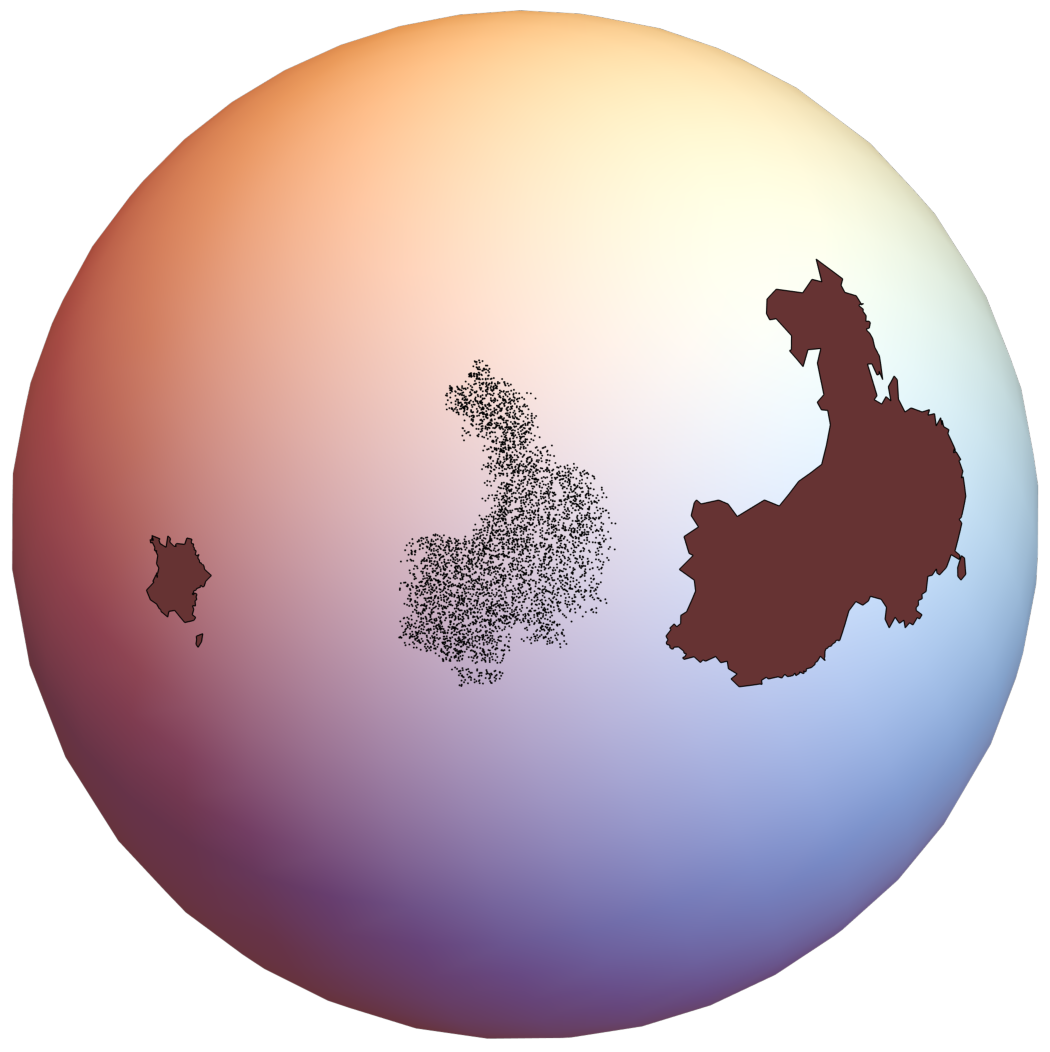
\includegraphics[width=\linewidth]{Chapters/OPT_sphere.pdf}
\end{wrapfigure}

In the right-hand side picture,
the author simulates the unique barycenter between the (mainland) country shapes of France and China.

\begin{example}[Barycenter between France and China]
	\label{example:barycenter_sphere}
	In this setting, $(E, d)$ is the Riemannian manifold of earth sphere.
	In the Wasserstein space $\mathcal{W}_2(E)$, consider two uniform measures $\mu$ and $\nu$,
	with supports on the maps of France and China respectively.
	The aim is to simulate the (unique) barycenter $\eta$ of $\frac{1}{2}\delta_\mu + \frac{1}{2}\delta_\nu$.
	With the help of \cref{thm:geodesic_Wasserstein_space}, we proceed as following.
	We simulate 5000 points for measures $\mu$ and $\nu$.
	Then we compute an optimal matching between those points,
	which costs more than 5 hours in the author's laptop.
	Given these 5000 pairs of points,
	we draw their (unique) barycenters on the sphere and that is a simulation of desired barycenter measure $\eta \in \mathcal{W}_2(E)$.
\end{example}

The source code is shared as a \href{https://www.wolframcloud.com/obj/jingmatrix/Published/OPT_sphere_country.nb}{Wolfram Notebook}.

\section{Existence and consistency}

Results in this section is fully borrowed from \cite{le2017existence}.
We present them in a more geometrical style without the purpose of claiming originality.

Wasserstein space is not locally compact unless the base space is compact (\cite[Remark 7.1.9]{Ambrosio2005}).
But weakly convergence behaves well with Wasserstein metric, and we can get weakly compactness with less cost.
Properness of base space gives ``properness'' of Wasserstein space for \underline{weakly convergence topology}.

\begin{prop}
	\label{prop:proper_weakly_convergence_topology}
	For a proper space $(E,d)$,
	every bounded set in $\mathcal{W}_p(E)$ is tight and thus
	sequentially	pre-compact in weakly convergence topology.
\end{prop}

\begin{proof}
	Closed ball $B(x,r)$ is compact in $E$.
	By Markov inequality,
	\[
		\mu(E - B(x,r)) = \int_{E - B(x,r)} \diff \mu \leq
		\int_{E} \frac{d(x, y)^p}{r^p} \diff \mu(y) \leq  \frac{W_p(\mu, \delta_x)^p}{r^p},
	\]
	and we conclude by the assumption that $W_p( \mu, \delta_x)$ is bounded.
\end{proof}

By abuse of language, we drop $\delta$ symbol in following discussion when there is no ambiguity.
This convention is indicated in \cref{subsection:convention}.
\begin{thm}[Consistency of barycenter in Wasserstein space]
	\label{thm:consistency_barycenter_Wasserstein}
	Let $(E,d)$ be a proper space and $\mathbb{P}_n$  be a sequence in $\mathcal{W}_p(\mathcal{W}_p(E))$
	with barycenter $\mu_n \in \mathcal{W}_p(E)$ and $\mathbb{P}_n \rightarrow \mathbb{P}$ with respect to Wasserstein metric.

	Then $\mu_n$ is tight and any weakly convergence limit $\mu$ of $\mu_n$ will be a barycenter of $\mathbb{P}$.
	Moreover, we have $W_p(\mu_n, \mu) \rightarrow 0$.
\end{thm}

\begin{proof}[Proof: $\mu$ is barycenter]
	By \cref{prop:proper_weakly_convergence_topology} we firstly show that the sequence $\mu_n$ is bounded.
	To show that barycenters of bounded set is bounded, by abuse of notation,
	pick a $x \in E$ and use the assumption that $\mu_n$ is barycenter of $\mathbb{P}_n$,
	\[
		W_p(\mu_n, x) \leq W_p(\mu_n, \mathbb{P}_n)  + W_p(\mathbb{P}_n, x) \leq 2 W_p(\mathbb{P}_n , x).
	\]
	And the last item is bounded as $\mathbb{P}_n$ is a converging sequence.

	From continuity of Wasserstein distance we have
	\[
		W_p(\mathbb{P}, \mathcal{W}_p(E)) =
		\lim_{n \rightarrow \infty}W_p(\mathbb{P}_n, \mathcal{W}_p(E))=\lim_{n \rightarrow \infty}W_p(\mathbb{P}_n, \mu_n)
		= \lim_{n \rightarrow \infty}W_p(\mathbb{P}, \mu_n);
	\]
	then by lower semi-continuity of Wasserstein distance for weakly convergence
	\[
		W_p(\mathbb{P}, \mathcal{W}_p(E)) =
		\lim_{n \rightarrow \infty}W_p(\mathbb{P}, \mu_n)
		\geq W_p(\mathbb{P}, \mu).
	\]
	Hence, $W_p(\mathbb{P}, \mathcal{W}_p(E)) =W_p(\mathbb{P}, \mu)$.
\end{proof}

We have shown that $W_p(\mathbb{P}, \mu_n) = W_p(\mathbb{P}, \mu)$.
And from following proposition that previous weakly convergence is in fact convergence in Wasserstein metric.

\begin{prop}
	For a weakly convergence sequence $\mu_n \rightharpoonup \mu$,
	the following condition are sufficient and necessary (hence equivalent) to have $\mu_n \rightarrow \mu$ convergence in Wasserstein metric.
	\begin{enumerate}
		\item $W_p(\mu_n, x) \rightarrow W_p(\mu, x)$ for an element $x$ in $E$.
		\item $W_p(\mu_n, \nu) \rightarrow W_p(\mu, \nu)$ for an element $\nu$ in $\mathcal{W}_p(E)$.
		\item $W_p(\mu_n, \mathbb{P}) \rightarrow W_p(\mu, \mathbb{P})$ for an element $\mathbb{P}$ in $\mathcal{W}_p(\mathcal{W}_p(E))$.
	\end{enumerate}
\end{prop}

That is say,
from weakly convergence to Wasserstein convergence,
what we need in addition is the convergence of Wasserstein distance with respect to a point
either in $E$, $\mathcal{W}_p(E)$ or $\mathcal{W}_p(\mathcal{W}_p(E))$.

\begin{proof}
	The first point is stated in \cref{thm:Wp_metricizes_weak_convergence}.
	And	the second point is proved technically in \cite[Lemma 14]{le2017existence}.
	We prove that last one using the second one.

	Take $\hat{\mu}$ a random probability measure with law $\mathbb{P}$,
	by lower semi-continuity of Wasserstein metric with respect to weakly convergence we have
	\begin{align*}
		\mathbb{E}W_p(\mu, \hat{\mu}) & =W_p(\mu, \mathbb{P})=\lim_{n \rightarrow \infty} W_p(\mu_n, \mathbb{P}) \\
		                              & \geq \mathbb{E}\liminf_{n \rightarrow \infty} W_p(\mu_n, \hat{\mu})      \\
		                              & \geq \mathbb{E}W_p(\mu, \hat{\mu}).
	\end{align*}
	The first inequality results from Fatou's lemma.
	From calculation above these two inequalities are in fact equalities.
	A subsequence of $\mu_n$ will satisfy these equalities as well.
	We can then prove by contradiction that $\liminf$ above can be safely substituted by $\lim$.
	That is to say,
	\[
		\mathbb{E}W_p(\mu, \hat{\mu}) = \mathbb{E}\lim W_p(\mu_n, \hat{\mu}),
		\quad W_p(\mu, \hat{\mu}) \leq \liminf_{n \rightarrow \infty} W_p(\mu_n, \hat{\mu})
	\]
	Therefore, we have almost everywhere that $\lim W_p(\mu_n, \hat{\mu})=W_p(\mu, \hat{\mu})$.
\end{proof}

The set of measures with finite support is dense in Wasserstein space by \cref{thm:topology_Wasserstein}.
Our final step to the existence of barycenter in Wasserstein space over a proper space
is to prove it for measures with finite support.

\begin{thm}
	\label{thm:barycenter_finite_support_measure}
	Let $(E,d)$ be a proper space.
	In $\mathcal{W}_p(E)$, barycenter of probability measure with finite support,
	hence of any element in $\mathcal{W}_p(\mathcal{W}_p(E))$,
	exists.
\end{thm}

\begin{proof}
	Let $\lambda_i$ be $n$ given positive coefficients with sum $1$,
	$\mu_i$ be $n$ given measures on $(E,d)$.
	We aim to find a solution for following optimization problem
	\[
		\min_{\nu} \sum_{i=1}^{n}\lambda_i W_p(\nu, \mu_i)^p.
	\]
	For a given $\nu$, let $(X, X_1,\ldots,X_n)$ be a choice of random variable with value in $E^{n+1}$ such that $(X,X_i)$ is an optimal coupling for $\nu$ and $\mu_i$. We thus have $\mathbb{E}d(X,X_i)^p = W_p(\nu, \mu_i)^p$.

	Denote $\boldsymbol{x}=(x_1, x_2, \ldots, x_n) \in E^n$ and define $f(\boldsymbol{x}):= W_p(\eta, E)^p$,
	where $\eta := \sum_{i=1}^{n} \lambda_i \delta_{x_i}$.
	We use ``$\min$'' in this definition because barycenter of measures in $E$ always exists.

	Denote $\Gamma$ the set of all possible choice of $(X_1, \ldots, X_n)$, we have
	\begin{align*}
		\sum_{i=1}^{n}\lambda_i W_p(\nu, \mu_i)^p & = \mathbb{E} \sum_{i=1}^{n}\lambda_i d(X,X_i)^p  \\
		                                          & \geq \mathbb{E} f(X_1, \ldots, X_n)              \\
		                                          & \geq \inf_\Gamma \mathbb{E} f(X_1, \ldots, X_n).
	\end{align*}
	We shall show that these two inequalities can be in fact equalities.

	For the second one, the existence of solution to this minimization problem over $\Gamma$
	is a multi-marginal optimal transportation problem with cost function $f$.
	Inspired by the proof of existence of optimal plan in \cref{thm:existence_optimal_coupling},
	we should first show that $\Gamma$ is weakly compact.
	$\Gamma$ is tight as elements in it have given marginal distributions;
	here we use a multi-marginal version of \cref{lem:tightness_transference_plan}.
	$\Gamma$ is weakly closed by stability of optimal plans,
	which is guaranteed by lower semi-continuity of transport cost with respect to weakly convergence,
	i.e., \cref{lem:lower_semi-continuity_of_the_cost_functional}.

	We show that $f$ is continuous.
	Recall $\eta= \sum_i^{n}\lambda_i \delta_{x_i} \in \mathcal{W}_p(E)$, observe that sequence convergence of $\boldsymbol{x}$ in $E^n$ corresponds to weakly convergence of $\eta$.
	By definition $f(\boldsymbol{x}) = W_p(\eta, E)^p=W_p(\eta, y)^p = \sum_{1}^{n} \lambda_i d(y, x_i)^p$
	for some barycenter $y$ of $\eta$ in $E$.
	Let $\eta_j$ be a sequence of measures of such form corresponding to $\boldsymbol{x}_j$ and
	let $y_j$ be a barycenter of $\eta_j$.

	We firstly show that $y_i$ is sequentially pre-compact.
	Recall that bounded set in Wasserstein space is
	weakly sequentially pre-compact in \cref{prop:proper_weakly_convergence_topology}
	and weakly convergence of Dirac measures has the same topology as base space.
	Hence, we only need to show that $y_i$ is bounded is the Wasserstein space $\mathcal{W}_p(E)$.
	This comes from that $\eta_j$ is bounded and barycenters of bounded set is bounded as we proved in \cref{thm:consistency_barycenter_Wasserstein}.
	For now, if $y_j \rightarrow y$ up to a subsequence for some $y \in E$, then
	\[
		\lim f(\boldsymbol{x_i}) := \lim W_p(\eta_j, E) = \lim W_p(\eta_j, y_j) =  W_p(\eta, y) =: f(\boldsymbol{x}),
	\]
	since $W_p(\eta_j , y_j)$ is just a convex combination of distances and
	$\boldsymbol{x}_j \rightarrow \boldsymbol{x}$.
	It is necessary that $y$ is a barycenter of $\eta$ as a limit of $y_j$,
	since for a barycenter $z$ of $\eta$ we can pass to the limit in $W_p(\eta_i, z) \geq W_p(\eta_i, E)$.
	This shows that $f(\boldsymbol{x})$ is continuous with respect to $\boldsymbol{x}$ since
	any sequence of $f(\boldsymbol{x_i})$ has a subsequence converging to $f(\boldsymbol{x})$.

	For the first inequality,
	we need to show the existence of a measurable function $B(\boldsymbol{x}) \in \arg \min_{x \in E} \sum_{i=1}^{n} \lambda_i d(x, x_i)^p$.
	We shall apply remarkable Kuratowski and Ryll-Nardzewski measurable selection theorem (\cite[Theorem 6.9.3]{Bogachev2007}),
	see it also on \href{https://en.wikipedia.org/wiki/Kuratowski_and_Ryll-Nardzewski_measurable_selection_theorem}{Wikipedia}.
	We define
	\begin{align*}
		\Gamma^\varepsilon:                   & =	\{
		(y,\boldsymbol{x}) \in E^{n+1} \mid  f(\boldsymbol{x}) - \sum_{i=1}^{n} \lambda_i d(y,x_i)^p < \varepsilon
		\}, \quad \varepsilon > 0                                                                           \\
		\Gamma^0:                             & =	\{
		(y,\boldsymbol{x}) \in E^{n+1} \mid  f(\boldsymbol{x}) - \sum_{i=1}^{n} \lambda_i d(y,x_i)^p = 0
		\},                                                                                                 \\
		\Gamma^\varepsilon_{\boldsymbol{x}} : & = \{ y \mid (y, \boldsymbol{x} ) \in \Gamma^\varepsilon \},
		\quad \varepsilon \geq 0.
	\end{align*}
	To apply the measurable selection theorem,
	we should show that for any open set $U \subset E$, the set
	$\{ \boldsymbol{x} \mid \Gamma^0_{\boldsymbol{x}} \cap U \ne \emptyset \}$
	is measurable.
	Denote $\pi: (y , \boldsymbol{x}) \in E^{n+1} \mapsto  \boldsymbol{x} \in E^n$ the projection,
	which is an open map.
	We conclude by following calculation,
	\[
		\{ \boldsymbol{x} \mid \Gamma^0_{\boldsymbol{x}} \cap U \ne \emptyset \} =
		\cap_{\varepsilon \downarrow 0}
		\pi ( \Gamma^\varepsilon \cap U \times E^n ).
	\]

	For our proof, to be concrete,
	let $\boldsymbol \gamma$ be a solution to the second inequality,
	that is to say,
	an optimal transference plan with marginals $\mu_i$ with respect to (continuous) cost function
	$f(\boldsymbol{x}):=\min_{x} \sum_{i=1}^{n} \lambda_i d(x, x_i)^p = : W_p(\sum_{i=1}^n \lambda_i \delta_{x_i}, E)^p$.
	Then $\mu:= B_{\#}\boldsymbol \gamma$ is a barycenter of $\sum_{i=1}^{n}\lambda_i \delta_{\mu_i}$.
\end{proof}

\begin{rmk}
	\label{rmk:barycenter_compact}
	Let $\boldsymbol{A} \subset E^n$ be a compact set.
	All barycenters of $\sum_{i=1}^n \lambda_i \delta_{x_i}$ when $\boldsymbol{x}$ runs through $\boldsymbol{A}$,
	denoted by $\operatorname{bary}( \boldsymbol{A} )$,
	\[
		\operatorname{bary}( \boldsymbol{A} ) :
		=\{y \mid (y, \boldsymbol{x}) \in \Gamma^0, \boldsymbol{x} \in \boldsymbol{A} \}
		= \pi ( \Gamma^0  \cap E \times \boldsymbol{A})
	\]
	is compact.
	It is closed since $\pi$ is an open map.
	It is bounded since barycenters are located in the union of $n$ bounded balls with centres $x_i$.
\end{rmk}


%! TEX root = ../barycenter.tex
\YYCleverefInput{/var/tmp/latex/barycenter.sed}
\chapter{The case of Wasserstein space over Riemannian manifold}

We continue to use the notation in the proof of last \Cref{thm:barycenter_finite_support_measure}.
There is a measurable function $B$ from $n$ points $x_i \in E$ to a barycenter of $\sum_{i=1}^{n} \lambda_i \delta_{x_i}$;
and we have shown that
\[f(\boldsymbol{x}) :=W_p(\sum_{i=1}^n \lambda_i \delta_{\mu_i}, E)^p =\min_{x \in E} \sum_{i=1}^n \lambda_i d(x, x_i)^p\]
is continuous.
For the study in the case when $E$ is a complete manifold $M$,
we set $p = 2$ and apply some possible (non-)smooth analysis.
To begin with, we shall establish some fine properties of two functions $f$ and $B$.
% As an infimum involution, $f$ is locally Lipschitz;
% while $B$, not necessarily continuous, shares similar properties as optimal transport maps
% and we should talk about their differentiability only with respect to some reference measure.
As we shall see later from \cref{equa:formula_barycenter},
% both optimal transport map $T$ in \Cref{thm:uniquness_monge_problem_manifold} and
barycenter map $B$
has the form $\exp( - \nabla h)$ for some $c$-concave
function $h$ that is differentiable almost everywhere with respect to the volume measure.
% \section{Details for analysis on manifolds}
\section{\texorpdfstring{$c$}{c}-concave function}

Most content in this section is a copy-paste from \cite{cordero2001riemannian},
detailed proofs and references are given therein.
From now on, $M$ is always a complete Riemannian manifold.
% But $ \nabla h$ is not defined everywhere.
% And even for compact manifold $M$,
% $\exp( - \nabla h)$ as an optimal transport map could be discontinuous.
% A proper definition of the differential $\diff \exp(- \nabla h)$,
% of course only possible almost everywhere,
% is the main goal of this section.

% \subsection{Differentiate squared distance function}


Both $f$ and $B$, and even optimal transport plan are related to so-called $c$-concave functions.
For $x,y \in M$, we define a function $c(x,y): = \frac{1}{2} d^2(x,y)$ as the half of distance between $x$ and $y$.

\begin{defn} [$c$-transforms and the subset \( \mathcal { I } ^ { c } ( X , Y ) \) of \( c \)-concave functions]
	Let \( X \) and \( Y \) be two compact subsets of \( M \).
	The set \( \mathcal{I} ^ { c } ( X , Y ) \) of \( c \)-concave functions (relative to \( X \) and \( Y \)) is
	the set of functions \( \phi \) : \( X \rightarrow \mathbb { R } \cup \{ - \infty \} \) not identically \( - \infty \),
	for which there exists a function \( \psi : Y \rightarrow \mathbb { R } \cup \{ - \infty \} \) such that
	\begin{equation}
		\label{defn:c_transform}
		\phi ( x ) = \inf _ { y \in Y } c ( x , y ) - \psi ( y ) \quad \forall x \in X.
	\end{equation}
	We refer to \( \phi \) as the \( c \)-transform of \( \psi \) and abbreviate \cref{defn:c_transform}
	by writing \( \phi = \psi ^ { c } \).
	Similarly, given \( \phi \in \mathcal{I} ^ { c } ( X , Y ) \),
	we define its \( c \)-transform \( \phi ^ { c } \in \mathcal{I} ^ { c } ( Y , X ) \) by
	\begin{equation}
		\label{equa:c_transform_of_c_conjugate}
		\phi ^ { c } ( y ) : = \inf _ { x \in X } c ( x , y ) - \phi ( x ) \quad \forall y \in Y.
	\end{equation}
\end{defn}

We hope no confusion results from the tacit dependence of
these transformations on the domain of the function being transformed.
For \( \phi \in \) \( \mathcal { I } ^ { c } ( X , Y ) \),
it follows easily from \cref{equa:c_transform_of_c_conjugate} as in Rachev and Rüschendorf
\cite[Section 3.3]{Rachev1998} that
\[ \phi ( x ) = \inf _ { y \in Y } c ( x , y ) - \phi ^ { c } ( y ) \quad \forall x \in X \]
which we abbreviate by writing \( \phi ^ { c c } = \phi \), suppressing the domains of definition once more.
As in \cite{mccann2001polar}, Lipschitz continuity of \( \phi ^ { c } \) follows merely from
compactness of \( X \) and the locally Lipschitzian character of \( c ( x , y ) \),
regardless of whether or not \( \phi : X \rightarrow \mathbb { R } \cup \{ - \infty \} \) is continuous.
Thus, it costs no generality to
assume \( \psi \) and \( \phi \) are continuous and real-valued in \cref{defn:c_transform}.

For any \( y \in M \), we denote by \( d _ { y } ( \cdot ) : = d ( \cdot , y ) \)
the distance function to \( y \).
\begin{example}[$d^2_y(x)$ is a $c$-concave function]
	\label{example:square_distance_c-concave}
	For two compact sets $X,Y \subset M$, we fix a $y \in Y$ then
	$d^2_y(\cdot) \in \mathcal{I}^c (X,Y)$ for a fixed $y$ is a $c$-concave function.
	Because we can define a desired $\psi$ by setting $\psi (y) := 0$ and $\psi (z) := - \infty$ for $ z \neq y, z \in Y$.
\end{example}

% Let us also recall one of the basic lemmas from its proof,
% which illuminates the structure of the map \( T \).
Given two compact subsets \( X \) and \( Y \subset M \) with \( \phi \in \mathcal { I } ^ { c } ( X , Y ) \),
one sees every \( ( x , y ) \in X \times Y \) satisfy
\begin{equation}
	\label{equa:c-concave_conjugate}
	c ( x , y ) - \phi ( x ) - \phi ^ { c } ( y ) \geq 0
\end{equation}
with equality when \( \phi ( x ) = \inf _ { y ^ { \prime } \in Y } c \left( x , y ^ { \prime } \right) - \phi ^ { c } \left( y ^ { \prime } \right) = c ( x , y ) - \phi ^ { c } ( y ) . \)

The following lemma \cite[Lemma 3.2]{cordero2001riemannian} is fundamental in sequel discussion,
detailed proofs can be found in \cite[Lemmas 2 and 7]{mccann2001polar}.
\begin{lem}
	[Elementary properties of \( c \)-concave functions]
	\label{lem:minimizer_differentiable}
	Fix \( \mathcal{X} \subset \subset M \) open and \( Y \subset M \) compact,
	where $ \mathcal{X} \subset \subset M $ means that $\mathcal{X}$ is a pre-compact subset of $M$.
	For \( \phi \in \mathcal{I} ^ { c } ( \widebar { \mathcal{X} } , Y ) \) define \( F ( x ) : = \)
	\( \exp _ { x } ( - \nabla \phi ( x ) ) \).
	\begin{enumerate}
		\item The function \( \phi \) is Lipschitz on \( \widebar { \mathcal{X} } \) and
		      hence differentiable almost everywhere on \( \mathcal{X} \) with respect to the volume measure.
		\item Fix any point \( x \in  \mathcal{X} \) where \( \phi \) is differentiable. Then \( y = F ( x ) \) if and
		      only if \( y \) minimizes \cref{equa:c-concave_conjugate} among \( y ^ { \prime } \in Y . \) In the latter case one has
		      \( \nabla \phi ( x ) = \nabla d _ { y } ^ { 2 } ( x ) / 2 \).
	\end{enumerate}
\end{lem}

As we mentioned in \Cref{example:square_distance_c-concave},
the squared distance function $d^2_y(\cdot)$ is a $c$-concave function and \Cref{lem:minimizer_differentiable} applies.
And it turns out that conclusions from this lemma is quite natural from the perspective of cut locus.

\subsection{Reminder for cut locus}

For \( x \in M \), the \emph{cut locus} refers to the set \( \operatorname{cut}( x ) \subset M \) of all \( z \in M \) which
which do not belong to the (relative) interior of a minimizing geodesic going
through $x$.
% cannot be linked to \( x \) by an extendable minimizing geodesic.
The exponential map \( \exp _ { x } : T _ { x } M \rightarrow M \) is differentiable
at any tangent vector \( v \in T _ { x } M \) satisfying \( \exp _ { x } v \notin \operatorname{cut}( x )\),
and its differential \( \diff \left( \exp _ { x } \right) _ { v } \) gives a linear bijection between the tangent
spaces \( T _ { x } M \) and \( T _ { \exp _ { x } v} M\).
We mention that the cut locus $\operatorname{cut} (x)$ is a closed set with measure zero with respect to the volume measure.

The relationship between distance function $d_y(\cdot) : = d(\cdot, y) $ and the
exponential map is summarized by the formula \( d _ { y } \left( \exp _ { y } v \right) = | v | \),
which holds for any \( v \) from the star-shaped domain around \( 0 \in T _ { y } M \)
which does not intersect \( \left( \exp _ { y } \right) ^ { - 1 } [ \operatorname{cut} ( y ) ]\).
This shows the exponential map generates the minimal geodesics through \( y \),
and that the function \( d _ { y } ^ { 2 } / 2 \) is smooth around any \( x \notin \operatorname{cut} ( y ) \).
Where \( d _ { y } ^ { 2 } / 2 \) is differentiable,
its gradient is related to the exponential map by the formula
\begin{equation}
	\label{equa:exponential_map_and_squared_distance_function}
	y = \exp _ { x } \left[ - \nabla d _ { y } ^ { 2 } ( x ) / 2 \right],
\end{equation}
and for \( x \notin \operatorname { cut } ( y ) \) its Hessian \( H = \operatorname{ Hess} _ { x } d _ { y } ^ { 2 } / 2 \) can be viewed either as a symmetric quadratic form on \( T _ { x } M \) or as a self-adjoint operator
\( H : T _ { x } M \rightarrow T _ { x } M \).
Note that \cref{equa:exponential_map_and_squared_distance_function} requires the existence of
a minimal geodesic linking \( x \) to \( y \),
and it is for this reason that completeness of the manifold is required.

In the sequel, it proves useful to characterize the cut locus \( \operatorname { cut } ( y ) \) as
the set of points where the distance function \( d _ { y } ^ { 2 } / 2 \) must fail to be smooth.
As mentioned above,
\( d _ { y } ^ { 2 } / 2 \) is as smooth as the manifold away from the cut locus of \( y \).
But \( \operatorname{cut} ( y ) \) consists of two kinds of points:
\begin{enumerate}
	\item those connected to \( y \) by multiple minimizing geodesics, and
	\item	those which are conjugate to \( y \) but do not fall into the first class.
\end{enumerate}
The point of the following proposition \cite[Proposition 2.5]{cordero2001riemannian}
is that differentiability of \( d _ { y } ^ { 2 } \) must fail --- at first order in the first case,
and at second order in the second case.
Moreover, the failure occurs with a definite sign:
the Hessian diverges to $-\infty$ while remaining bounded above, according to \Cref{lem:hessian_bound_distance_squared}.

\begin{prop}
	[Distances fail to be semi-convex at the cut locus]
	\label{prop:distance_cut_locus}
	At each \( x \in \operatorname { cut } ( y ) \), the square distance \( d _ { y } ^ { 2 } / 2 \) satisfies:
	\[ \inf _ { 0 < | v | < 1 } \frac { d_y^2 \left( \exp _ { x } v \right) + d_y^2 \left( \exp _ { x } - v \right)
		- 2 d_y^2 ( x ) } { | v | ^ { 2 } } = - \infty \]
\end{prop}

%! TEX root = ../barycenter.tex
\YYCleverefInput{/var/tmp/latex/barycenter.sed}
\section{Barycenter in manifold}

\label{section:barycenter_manifold}
Recall that we define $c(x, y):=\frac{1}{2} d(x, y)^2$;
and for $n$ points $x_j \in M, j=1,2,\ldots,n$, now we re-define $f$ on $M^n$ with a coefficient $\frac{1}{2}$
to make later notations easier,
\[
	f(x_1, x_2, \ldots, x_n) := \min_{w} \sum_{j=1}^n \lambda_j c(w, x_j) =: \frac{1}{2}W^2(\sum_{j=1}^n \lambda_j \delta_{x_j}, M).
\]
We remark that this re-definition affects nothing in we discussed before.

Pick an $i, 1 \leq i \leq n$ such that $\lambda_i \neq 0$, then we fix $x_j$ for $j \neq i$ and
define $f_i (x_i) : = f(x_1, \ldots, x_n)$.
Take an arbitrary open pre-compact neighbourhood $\mathcal{X} \subset \subset M$ of $x_i$;
let $Y$ the set of all barycenters of $\sum_{j=1}^n \lambda_j \delta_{x_j}$
when $x_i$ runs through in $\widebar{ \mathcal{X} }$.
Then $Y$ is compact by \Cref{rmk:barycenter_compact}.
% Consider a $c$-concave function $ g_i \in \mathcal{I}(Y, \widebar{ \mathcal{X} })$
% \[
% 				g_i(w) := - \frac{1}{\lambda_i} \sum_{j\neq i}^n \lambda_j c( x_j, w)  =
% 				\inf_{x_i \in \widebar{ \mathcal{X} }}c( x_i, w ) -
% 				\frac{1}{\lambda_i} \sum_{j=1}^n \lambda_j c( x_j, w),
% \]

We define $g_i(w): = - 1/ \lambda_i \sum_{j \neq i} \lambda_j c(w, x_j) $ on $M$,
then by definition $f_i /\lambda_i \in \mathcal{I}^c (\widebar{ \mathcal{X}}, Y)$
is the $c$-transform of
$g_i$ restricted to $Y$.
The $c$-transform inequality
$ c(w, x_i) \geq g_i(w) + f_i / \lambda_i (x_i)$
becomes equality when $z$ is a barycenter of $\sum_{i=1}^{n} \lambda_i \delta_{x_i}$,
\begin{equation}
	\label{equa:g_i_conjugate}
	c(z, x_i) = g_i(z) + \frac{1}{\lambda_i} f_i(x_i).
\end{equation}

\begin{rmk}[$g_i$ on $Y$ is the $c$-transform of $f_i / \lambda_i$]
	In general, we have by definition of $c$-transform that
	$g_i(w) \leq (f_i / \lambda_i)^c(w) := \inf_{x_i \in \widebar{ \mathcal{X} } } c(x_i, w) - f_i / \lambda_i (x_i)$.
	If $ c(z, x_i) = g_i (z) + f_i / \lambda_i (x_i)$,
	then
	$g_i(z) = (f_i / \lambda_i)^c (z)$ since $(f_i / \lambda_i)^c(z) + f_i / \lambda_i(x_i) \leq c (z, x_i)$.
	This implies that $g_i = (f_i / \lambda_i)^c$ on $Y$.
	% If $g_i$ is differentiable then $f_i / \lambda_i \geq g_i$ is sub-differentiable
	% and thus differentiable with the same gradient as $g_i$.
	% So $(f_i / \lambda_i)^c$ is differentiable on $Y$.
	% By \Cref{example:minimizer_differentiable}, for each barycenter $z \in Y$,
	% there exists a unique $x_i = \exp_z (- \nabla g_i (z))$ such that $z$ is the barycenter
	% of $\sum_{j=1}^n \lambda_j \delta_{x_j}$.
	% However, it says nothing on the uniqueness for barycenter of $\sum_{j=1}^n \lambda_j \delta_{x_j}$.
	% Both $g_i$ and $(f_i / \lambda_i)^c$ are continous;
	% $g_i$ is differentiable alomst everywhere with respect to volume measure.
	% because in local normal coordinate $g_i$ is differentiable almost everywhere
	% with respect to Lesbegue measure.
\end{rmk}

Moreover, \Cref{lem:minimizer_differentiable} tells us two things,
\begin{itemize}
	\item $f_i$ is Lipschitz on $\widebar{ \mathcal{X} }$;
	\item If $ \nabla f_i $ exists, then $z: = \exp( - \frac{1}{\lambda_i}\nabla f_i)$ is the
	      unique barycenter of $\sum_{i=1}^n \lambda_i \delta_{x_i}$.
\end{itemize}
Recall that $B$ is a measurable selection of barycenter of
measure $\sum_{j=1}^{n} \lambda_j \delta_{x_j}$ on $M$.
% that is to say,
% \[
% B(\boldsymbol{x}) \in \arg \min_{w \in M} \sum_{i=1}^{n} \lambda_i d(w, x_i)^2.
% \]
We have the following \textbf{barycenter formula}
if $f_i$ is differentiable at $x_i$,
\begin{equation}
	\label{equa:formula_barycenter}
	B(x_1, x_2, \ldots, x_n) = \exp_{x_i} (- \frac{1}{\lambda_i} \nabla f_i(x_i)).
\end{equation}

The barycenter formula \cref{equa:formula_barycenter} expresses the fact that,
from point $x_i$,
we can reach barycenter of $\sum_{j=1}^n \lambda_i \delta_{x_j}$ if we follow the direction $-\nabla f_i$
and advance $\| \nabla f_i / \lambda_i \| $.
In the case of Euclidean space,
\[
	\frac{1}{\lambda_i} \nabla f_i(x_i) = x_i - \sum_{j=1}^n \lambda_j x_j;                              \quad
	\nabla g_i(w)  = \frac{1}{\lambda_i} (w - \sum_{j=1}^n \lambda_j x_j) -(w-x_i).
\]


The following fine property of barycenter is stated in \cite[Lemma 3.1]{kim2015multi}.
We emphasize the fact that this lemma connects the notion of barycenter with geometry of our manifold $M$.
\begin{lem}
	\label{lem:barycenter_out_of_cut_locus}
	Fix \( \left( x _ { 1 } , \ldots , x _ { n } \right) \in M^n\).
	Then any barycenter $z$ of $\sum_{j=1}^n \lambda_j \delta_{x_j}$
	is not in the cut locus of \( x _ { j } \) for any \( j . \)
\end{lem}

\begin{proof}
	Choose a barycenter \( z \) in the cut locus of \( x _ { i } \) for some \( i \);
	we shall show that \( z \) cannot minimize
	\( y \mapsto \sum _ { j = 1 } ^ { n } d ^ { 2 } \left( x _ { j } , y \right) \).
	By \Cref{lem:hessian_bound_distance_squared} (for the sake of later convenience, we state it the next section) and compactness,
	we can find a constant \( K \) such that, for all \( u \in T _ { z } M \),
	and \( j = 1,2 , \ldots n \), we have
	\[
		\frac { d ^ { 2 }_{x _ { j } } \left(  \exp _ { z } u \right) + d ^ { 2 }_{x _ { j } } \left( \exp _ { z } ( - u ) \right) - 2 d ^ { 2 }_{ x_j} \left( z \right) }
		{ | u | ^ { 2 } } \leq K
	\]
	On the other hand, by \Cref{prop:distance_cut_locus},
	we can find some non
	zero \( u \in T _ { z } M \) such that
	\[
		\frac { d ^ { 2 }_{x _ { i } } \left(  \exp _ { z } u \right) + d ^ { 2 }_{x _ { i } } \left( \exp _ { z } ( - u ) \right) - 2 d ^ { 2 }_{ x_i} \left( z \right) }
		{ | u | ^ { 2 } } \leq - n K
	\]
	Therefore, we have
	\begin{align*}
		\sum _ { j = 1 } ^ { n } d ^ { 2 } \left( x _ { j } , z \right) & = \sum _ { j \neq i } ^ { n } d ^ { 2 } \left( x _ { j } , z \right) + d ^ { 2 } \left( x _ { i } , z \right)                                                                                                                   \\
		                                                                & \geq \frac { - ( n - 1 ) K | u | ^ { 2 } } { 2 } + \frac { 1 } { 2 } \sum _ { j \neq i } ^ { n } \left( d ^ { 2 } \left( x _ { j } , \exp _ { z } u \right) + d ^ { 2 } \left( x _ { j } , \exp _ { z } ( - u ) \right) \right) \\
		                                                                & + \frac { n K | u | ^ { 2 } } { 2 } + \frac { 1 } { 2 } d ^ { 2 } \left( x _ { i } , \exp _ { z } u \right) + d ^ { 2 } \left( x _ { i } , \exp _ { z } ( - u ) \right)                                                         \\
		                                                                & > \frac { 1 } { 2 } \sum _ { j = 1 } ^ { n } d ^ { 2 } \left( x _ { j } , \exp _ { z } u \right) + \frac { 1 } { 2 } \sum _ { j = 1 } ^ { n } d ^ { 2 } \left( x _ { j } , \exp _ { z } ( - u ) \right)
	\end{align*}
	Therefore, either
	\[ \sum _ { j = 1 } ^ { n } d ^ { 2 } \left( x _ { j } , \exp _ { z } u \right) < \sum _ { j = 1 } ^ { n } d ^ { 2 } \left( x _ { j } , z \right) \]
	or
	\[ \sum _ { j = 1 } ^ { n } d ^ { 2 } \left( x _ { j } , \exp _ { z } - u \right) < \sum _ { j = 1 } ^ { n } d ^ { 2 } \left( x _ { j } , z \right) \]
	in either case, \( z \) cannot minimize \( \sum _ { j = 1 } ^ { n } d ^ { 2 } \left( x _ { j } , z \right) \)
\end{proof}
This \Cref{lem:barycenter_out_of_cut_locus} implies that $g_i$ is differentiable at
any barycenter $z$ of $\sum_{j=1}^n \lambda_j \delta_{x_j}$.
% The \Cref{lem:barycenter_out_of_cut_locus} above tells that $g_i$ is differentiable at $z$.
% Since $z$ is not in the cut locus of $x_i$,
% $x_i$ is then not in the cut locus of $z$ and
% thus $c(z, x_i)$ is differentiable.
% If in addition, $f_i / \lambda_i$ is differentiable at $x_i$,
% then both hand side of \cref{equa:g_i_conjugate} are differentiable at $x_i$ and $z$.
Differentiating \cref{equa:g_i_conjugate} with respect to % $x_i$ and
$z$ and using the minimality property, we obtain,
\begin{align*}
	% z   & = \exp_{x_i}( - \frac{1}{\lambda_i} \nabla f_i), \\
	x_i & = \exp_{z}( - \nabla g_i).
\end{align*}
Therefore, $ \exp(- \nabla g_i) $ is a left inverse to $\exp( - \nabla f_i / \lambda_i)$,
\[
	\exp( - \nabla g_i) \circ \exp( - \frac{1}{\lambda_i} \nabla f_i) = \operatorname{Id},
	\quad \text{if } \nabla f_i \text{ exists}.
\]


\subsection{Uniqueness and curvature condition}

\label{section:uniqueness_and_curvature}

Whenever the barycenter formula \cref{equa:formula_barycenter} holds,
the barycenter of $\sum_{j=1}^n \lambda_j \delta_{x_j}$ is unique.
It means that non-uniqueness reveals the fact that the Lipschitz function
$f_i$ on $\widebar{ \mathcal{X} }$ is not \emph{a priori} differentiable.
In addition, on the set where $\nabla f_i$ exists, the map
$\exp( -\nabla f_i / \lambda_i )$ is injective.

In general, sufficient condition for uniqueness of barycenters of a probability measure $\mu$ on $M$
involves convex properties of distance function.
For example, in \Cref{prop:uniquness_barycenter_Wasserstein} we prove uniqueness of barycenter in Wasserstein space
from this perspective.
In \cite[Proposition IX.7.1]{chavel2006riemannian},
Ricci curvature bound from above plus bounded support for measure $\mu$ are used
to impose uniqueness of barycenter of $\mu$.
We could also use curvature condition for general length space as done by Ohta in \cite{ohta2012barycenters}.


%! TEX root = ../barycenter.tex
\YYCleverefInput{/var/tmp/latex/barycenter.sed}
\section{Barycenter in Wasserstein space}
\subsection{Uniqueness of barycenter measure}

We start with a description \cite[Theorem 10.41]{villani2008optimal}
for optimal mass transport on Riemannian manifold.
\begin{thm}[Uniqueness of optimal transport map for the square distance]
	\label{thm:uniquness_monge_problem_manifold}
	Let \( M \) be a Riemannian manifold, and \( c ( x , y ) = \frac{1}{2} d ( x , y ) ^ { 2 } \).
	Let \( \mu , \nu \) be two probability measures on \( M \), such that the optimal cost
	between \( \mu \) and \( \nu \) is finite.
	If \( \mu \) is absolutely continuous (with respect to volume measure $\operatorname{Vol}$ on $M$),
	then the mass transport
	problem between \( \mu \) and \( \nu \) admits a unique optimal transport plan, and it
	has the form \( \diff \pi ( x , y ) = \diff \mu ( x ) \delta [ y = T ( x ) ] \),
	or equivalently \[ \pi = ( \mathrm { Id } \times T )_{\#} \mu , \]
	where \( T \) is uniquely determined, \( \mu \)-almost everywhere,
	by the requirements that \( T_{\#} \mu = \nu \).
\end{thm}

The map \( T \) may be referred as
the optimal (mass) transport map pushing \( \mu \) to \( v \).
% Recall that in \Cref{thm:optimal_transport_manifold} we gave a description of $T$
% as $\exp_x(- \nabla \phi(x))$ when both $\mu$ and $\nu$ have compact supports.
With the help of this theorem, we are ready to prove
\begin{prop}
	\label{prop:uniquness_barycenter_Wasserstein}
	Given a measure $\mathbb{P} \in \mathcal{W}_2(\mathcal{W}_2(M))$,
	assume $\mathbb{P}$ gives mass to the set of absolutely continuous measures $P_{ac}(M) \subset \mathcal{W}_2(M)$,
	i.e.,	$\mathbb{P}(P_{ac}(M)) > 0 $.
	Then $\mathbb{P}$ has a unique barycenter in $\mathcal{W}_2(M)$, which is probability measure on $M$.
\end{prop}

\begin{rmk}
	$P_{ac}(M)$ is a Borel measurable subset of $(\mathcal{W}_2(M), W_2)$,
	see \cite[Proposition 2.1]{KIM2017640} for a proof.
\end{rmk}

\begin{proof}
	Note that any convex combination of elements the in space $\mathcal{W}_2(\mathcal{W}_2(M))$ is still inside it.
	The squared Wasserstein distance function $W^2_2(\mu, \cdot)$ is convex by definition of optimal plan,
	for $0 \leq \lambda_1, \lambda_2 \leq 1, \gamma_1 + \gamma_2 =1 $ and $ \nu_1,\nu_2 \in \mathcal{W}_2(M)$,
	\begin{equation}
		\label{equa:convexity_Wassersetein_distance}
		W_2^2(\mu, \lambda_1 \nu_2 + \lambda_2 \nu_2) \leq \lambda_1 W_2^2(\mu, \nu_1) + \lambda_2 W_2^2(\mu, \nu_2).
	\end{equation}

	And when $\mu \in \mathcal{W}_2(M)$ is absolutely continuous,
	we claim that inequality \cref{equa:convexity_Wassersetein_distance} becomes an equality only when
	$\lambda_1=0$ or $\lambda_2=0$,
	i.e.,
	convexity above becomes strict convexity.
	To prove this claim,
	according to \Cref{thm:uniquness_monge_problem_manifold} we write
	$\gamma_1 : = (\operatorname{Id}  \times T_1)_{\#}\mu$ the optimal plan from $\mu$ to $\nu_1$ and
	$\gamma_2 : = (\operatorname{Id}  \times T_2)_{\#}\mu$ the optimal plan from $\mu$ to $\nu_2$.

	Set $\gamma := \lambda_1 \gamma_1 + \lambda_2 \gamma_2$ for $\gamma_1, \gamma_2$ that turn
	\cref{equa:convexity_Wassersetein_distance} into equality,
	we have
	\begin{align*}
		\lambda_1 W_2^2(\mu, \nu_1) + \lambda_2 W_2^2(\mu, \nu_2) & = W_2^2(\mu, \lambda_1 \nu_2 + \lambda_2 \nu_2)            \\
		                                                          & \leq \int_{M \times M} d(x,y)^2 \diff \gamma(x,y)          \\
		                                                          & =	\lambda_1 W_2^2(\mu, \nu_1) + \lambda_2 W_2^2(\mu, \nu_2)
	\end{align*}
	Then $\gamma$ is an optimal plan from $ \mu$ to $\lambda_1 \nu_1 + \lambda_2 \nu_2$,
	but it cannot be induced by a map $T$ unless $\lambda_1 =0$ or $\lambda_2 =0$.

	After integrating \cref{equa:convexity_Wassersetein_distance} with respect to $\mathbb{P} \in \mathcal{W}_2(\mathcal{W}_2(M))$,
	we get a convex function
	\[\int_{\mathcal{W}_2(M)} W_2^2(\mu, \cdot) \diff \mathbb{P}(\mu),\]
	which is strictly convex if $\mathbb{P}$ gives mass to $P_{ac}(M)$, the set of absolutely continuous measures.
	Hence, the barycenter of $\mathbb{P}$ is unique.
\end{proof}

\subsection{Absolute continuity of barycenter for measures with finite support}

\label{section:absolute_continuity_finite_support}
Recall that in \Cref{thm:barycenter_finite_support_measure},
% we used consistency to prove existence of barycenter in the Wasserstein space
% $\mathcal{W}_p(E)$ over a proper space $E$.
we proved the existence of barycenter for measure $\sum_{j=1}^{n} \lambda_j \delta_{\mu_j}$ on $\mathcal{W}_p(E)$;
the barycenter we constructed is $B_{\#}\boldsymbol{\gamma} \in \mathcal{W}_p(E)$,
where $B$ is a measurable function from $n$ points $x_j \in E$ to a barycenter of
$\sum_{j=1}^{n} \lambda_j \delta_{x_j}$
and $\boldsymbol{\gamma}$ is an optimal plan with marginals $\mu_j$ with respect to the continuous cost function $f$.

We shall first show that barycenter of $\sum_{j=1}^n \lambda_j \delta_{\mu_j}$
is unique if some $\mu_i$
is absolutely continuous with respect to volume measure on the manifold $M$.
All main ideas in proving absolute continuity come from \cite{KIM2017640},
we basically re-write their proof in the following sections.
% We start with measure
% $\sum_{j}^{n} \lambda_{j} \delta_{\mu_j}$ on $\mathcal{W}_{2}(M)$.
% for $M$ a complete Riemannian manifold.
To use results and notation in \Cref{section:barycenter_manifold},
we fix $i = 1$ there.
Assume from now on \textcolor{cyan}{
	$ \lambda_1 \neq 0$ and that $\mu_1$ is absolutely continuous and
	concentrated in a pre-compact open set $ \mathcal{X} \subset M $
}.
Recall that we could define $f_1 \in \mathcal{I}^c( \widebar{ \mathcal{X} }, Y)$
as a $c$-concave function.
The barycenter measure $\widebar{\mu}$ of $\sum_{i}^{n} \lambda_{i} \delta_{\mu_i}$ is unique by \Cref{prop:uniquness_barycenter_Wasserstein}.
% because this measure gives mass to element in $P_{ac}(M)$.
% \subsubsection{One measure absolutely continous and others Dirac}
% We firstly consider the case when \textcolor{cyan}
\subsubsection{$\mu_i = \delta_{x_i}, i \geq 2$ are Dirac measures}

In this case, there is only one measure $\boldsymbol{\gamma}$ with marginals $\mu_i$.
As a consequence, $\exp(-\nabla f_1 / \lambda_1)$ pushes $\mu_1$ to $\widebar{\mu}$.
As a left inverse to $\exp(-\nabla f_1/\lambda_1)$,
\(\exp(-\nabla g_1)\) pushes $\widebar{\mu}$ to $\mu_1$.
Then $\widebar{\mu}$ is concentrated on the union of barycenters,
i.e., the compact set $Y$ by definition.
% We shall show soon $\exp(- \nabla g_1)$ could be almost everywhere Lipschitz
% with respect to volume measure if $M$ has lower bound for Ricci curvature.
% Now assume that is the case.
% This long inequality implies that any $w$ in the equality
% $c(x_i, w) = f_i / \lambda_i (x_i) + (f_i / \lambda_i)^c(w)$ must be a barycenter of $\sum_{i=1}^{n} \lambda_i \delta_{x_i}$.
% Moreover, we have following equality holds whenever one of gradients exits,
% \[\exp(-\nabla g_i) = \exp(-\nabla (f_i / \lambda_i)^c) = \exp^{-1}(-\nabla f_i / \lambda_i).\]
% Note cut-locus are excluded from consideration in above equality,
% and as a corollary $\nabla g_i = \nabla (f_i / \lambda_i)^c$.
% Therefore, two locally Lipschitz function $g_i$ and $f_i /\lambda_i$ coincide almost everywhere.
% If follows $g_i=f_i /\lambda_i$ on $M$.
% We discuss following in the sense of $\widebar{\mu}$ almost everywhere.
% The function $g_1$ is by definition just a sum of squared distance functions.
% Now we aim to find out when $ \exp(- \nabla g_1 )$ is a Lipschitz function.
% with Lipschitz constant depending only on $M$ and $\lambda_1$.
% As $M$ is compact, though tangent bundle $TM$ is not compact, local Lipschitz plus bounded diameter of $M$ implies global Lipschitz of $\exp$.
% Function $g_1$ has hessian upper bound by \Cref{prop:differentiate_optimal_transport},
% here we treat it as an infimal convolution over a fixed sigleton set $\{x_1\}$.
% Note that from $ \nabla g_1 = \nabla (f_1 / \lambda_1)^c$,
% $g_1$ and $(f_1 / \lambda_1)^c$ have the same hessian.
% Assume squared distance function has upper bound,
% then  $g_1$ has hessian upper bound as a $c$-conjugate function;
% function $g_1$ has hessian lower bound as a negative linear combination of square distance function.
% We then have
% \begin{equation}
% 	\label{equa:hessian_bound_f}
% 	-\frac{1-\lambda_1}{\lambda_1} H \leq \nabla^2 g_1, \qquad \nabla^2 (f_1 / \lambda_1)^c \leq H,
% \end{equation}
% where we denote by $H$ a possible bound from above for the hessian of square distance funtion.
% Recall that $H$ is bounded from above.
% Squared distance function $c$ has bounded Hessian from above.
% Hence $ \| \nabla^2 g \|$ is bounded from above by taking the second derivative of definition and also applying minimallity of cost at barycenter.
% Hence, we need two properties to have Lipschitzness of $\exp(-\nabla (f_1 / \lambda_1)^c)$:
% \begin{itemize}
% 	\item $ \exp $ is Lipschitz on the domain we are interested in.
% 	      % This would be the case when we are in the support of a compact supported function.
% 	      For example, in a compact domain.
% 	\item The hessian of square distance function has upper bound $H$.
% 	      This is the case when we have lower bound of sectional curvature.
% \end{itemize}
% We always take the second condition in following discussion.
% When $x_1$ runs through a bounded set,
% all possible barycenters are included in a bounded set.
% Hence $\widebar{\mu}$ has compact support.
% As we actually only consider measures with compact support, the first assumption is fullfilled as well.
% because $br$ pushes $\mu_1$ to $\widebar{\mu}$ by construction of $\widebar{\mu}$.
For $y \in Y$, $g_1$ is smooth by \Cref{lem:barycenter_out_of_cut_locus},
so $\exp( - \nabla g_1)$ is Lipschitz in a small open ball centring at $y$.
Choose a finite cover for $Y$ from these balls,
and denote by $C$ \underline{a global Lipschitz constant} of map \(\exp(-\nabla g_1)\) on $Y$.
Absolute continuity of $\mu_1$ means that given $\epsilon > 0$,
we can find a $\delta > 0$ such that $ \operatorname{Vol}(E) < \delta \implies \mu_1(E) < \epsilon$.
On the other hand, we have for measurable set $E$,
$\nabla g_1$ is well-defined on $E \cap Y$ and
$\operatorname{Vol}( \exp(- \nabla g_1 )( E \cap Y )) < C^n \operatorname{Vol}(E \cap Y)$
since volume measure is in fact a Hausdorff measure,
see \cite[Propositions 12.6 and 12.12]{TaylorMichaelEugene1946} for details.
Finally,
\begin{equation}
	\label{equa:absolutely_continuity_estimation}
	 \operatorname{Vol}(E) < \delta / C^n \implies \widebar{\mu}(E)
	=\mu_1(\exp(-\nabla g_1)(E \cap Y)) < \epsilon.
\end{equation}
Therefore, $\widebar{\mu}$ is absolutely continuous.
% Here the Lipschitz constant $C$ depends on the support of $\mu_1$.
% Since $\exp(-\nabla(f_1 / \lambda_1)^c) = \exp(-\nabla g_1) $ is continous for Vol-a.e. $x_1$
% (outside of cut-locus of $x_j, j \ne 1$),
% we deduce from absolute continuity of $\widebar{\mu}$ and compact support of $\mu_1$ that
% $\widebar{\mu}$ has also compact support.
% We have in general that the $c$-conjugate of $f_1 / \lambda_1$ satisfies
% $(f_1 / \lambda_1)^c = g_1^{cc} \geq g_1$,
% and thus $c(w, x_1) \geq (f_1 / \lambda_1)^c(w) + f_1/\lambda_1 (x_1) \geq g_1(w) + f_1/\lambda_1 (x_1)$.
% When $w$ is barycenter for some $x_1$,
% we have $g_1(w) = (f_1 / \lambda_1)^c(w)$.
% Hence, from the definition of $\widebar{\mu}$ we have
% $g_1 = (f_1 /\lambda_1)^c$ for $\widebar{\mu}$ alomost everywhere.
% And we have by minimallity that,
% $x_1 = \exp_w(- \nabla g_1(w)) = \exp_w(- \nabla (f_1 / \lambda_1)^c(w))$ once gradients exist.
% Therefore, we have $\nabla g_1 = \nabla (f_1 / \lambda_1)^c$ for volume measure almost everywhere.
% \begin{rmk}
% 	Once after we prove that $\widebar{\mu}$ is indeed absolutely continous.
% 	$\nabla g$ is invertable and $br(x_1) = \exp_{x_1} \nabla g^c(x_1)$.
% 	It is not surprised that
% 	\[
% g^c(x_1) = -c(x_1 ,z) - \frac{1}{\lambda_1} \sum_{i=2}^{n} \lambda_i\, c(x_i, z) =
% - \frac{1}{2 \lambda_1} W^2( \sum_{i=1}^n \lambda_i \delta_{x_i}, M),
% - f_1/\lambda_i.
% \]
% we can then take derivative with respect to $x_1$.
% \end{rmk}
% \subsubsection{To a more general case by conditional probability}
% \label{discussion_conditional_prob}
% To attack general case when \textcolor{cyan}{
\subsubsection{$\mu_i, i \geq 2$ are discrete measures}
To proceed with this slightly more general case,
we should consider (regular) conditional measures \cite[Section 10.4]{Bogachev2007} of an optimal multi-marginal transport plan $\gamma$
with marginals $\mu_i$:
\begin{equation}
	\label{equa:conditional_measure}
	\diff \gamma(x) = \gamma(\diff x \mid x^\prime)\, \diff \pi(x^\prime) ,
\end{equation}
where $x^\prime = (x_2, \ldots, x_n) \in M^{n-1}$ is the last $n-1$ coordinate components
of $x = (x_1, x_2, \ldots, x_n) \in M^n$ and
$\pi$ is the push-forward measure on $M^{n-1}$ from $\gamma$ by
the projection $x = (x_1, x^\prime) \mapsto x^\prime$.
As a definition \cite[Definition 10.4.1]{Bogachev2007}, \cref{equa:conditional_measure} means that,
\begin{enumerate}
	\item for $\pi$ almost everywhere $x^\prime$, $\gamma(\cdot \mid x^\prime)$ is a probability measure
	      concentrated on $M \times \{x^\prime\} \subset M^n$;
	\item for Borel sets $R \subset M^n$ , the function $ x^\prime \mapsto \gamma(R \mid x^\prime)$ is measurable and
	\item for Borel set $S \subset M^{n-1}$,
	      $\gamma(R \cap M \times S) = \int_{S} \gamma( R \mid x^\prime) \diff \pi(x^\prime)$.
\end{enumerate}

It follows that as a function on Borel subsets of $M$,
\begin{equation}
	\label{equa:push_forward_conditional_measure}
	\widebar{\mu}(\cdot) = B_{\#} \gamma (\cdot)= \int_{M^{n-1}} B_{\#} \gamma(\cdot \mid x^\prime)\, \diff \pi(x^\prime).
\end{equation}

If we show that for $\pi$ almost everywhere $x^\prime$ that
$B_{\#} \gamma(\cdot \mid x^\prime)$ is absolutely continuous,
then we could infer from \cref{equa:push_forward_conditional_measure} above that
$\widebar{\mu}(E)=0$ for any $\text{Vol}$-negligible set $E \subset M$ by integrating.
% \[
% 	\widebar{\mu}(E)
% =\int_{M^{n-1}}
% \frac{ \mu_1( br^{-1}(E) \cap A_{x^\prime} )}{\mu_1(A_{x^\prime})}
% \diff \pi(x^\prime)
% =\int_{M^{n-1}}
% \widebar{\mu}^{x^\prime}(E)
% \diff \pi(x^\prime)
% \leq \int_{M^{n-1}} C\,\mu_1^{\prime}(E) \diff \pi(x^\prime) \leq C\, \mu_1(E).
% = 0.
% \]

% Generally speaking, computation of $\gamma(\cdot \mid x^\prime)$ is only possible when
Heuristically, $\gamma(\diff x \mid x^\prime) = \diff \gamma(x) / \diff \pi (x^\prime)$ is a direct generalization of
classic conditional probability formula $P(A \mid B) = P(A B) / P(B)$.
For illustration, we calculate $\gamma(\cdot \mid x^\prime)$ in two cases,
\begin{itemize}
	\item $\pi$ is has finite support.
	      This is equivalent to that all $\mu_i, i \geq 2$ are discrete measures.
	      Fix any $x^\prime$ in the support of $\pi$ such that $\pi(\{x^\prime\}) >0$, by setting $S=\{x^\prime\}$ we get
	      \[
		      \gamma(\cdot \mid x^\prime) =
		      \frac{
			      \mathbbm{1}_{M \times \{x^\prime\}}
			      \gamma(\cdot)
		      }{\pi(\{x^\prime\})}.
	      \]
	\item $\gamma$ has density function $f: M^n \rightarrow \mathbb{R} $.
	      Then $\pi$ has density $\int_{M} f(x_1, x^\prime) \diff \operatorname{Vol}(x_1)$ and
	      \[
		      \gamma(\diff x \mid x^\prime) =
		      \frac{ f(x_1, x^\prime)} {\int_{M} f(x_1, x^\prime) \diff \operatorname{Vol}(x_1)}\diff \operatorname{Vol}(x)
	      \]
	      where we set the right hand side zero if it is indeterminate.
	      % and we remove this $x^\prime$ from consideration.
\end{itemize}
% Note in both cases, $\gamma(\cdot \mid x^\prime)$
% has absolutely continous push-forward measure
% $\mu_1^{x^\prime} := \text{proj}^1_{\#}\gamma(\cdot \mid x^\prime)$
% to the first coordinate.
But only in the first case that the measure $\gamma(\cdot \mid x^\prime) \leq \pi(x^\prime) \, \gamma(\cdot)$
is controlled by $\gamma$.
% Or we hope $f$ has positive lower bound,
% for example \textcolor{cyan}{continous and strictly positive}, like volume measure.
% In the case $\mu_1=\operatorname{Vol}$? Every point in $\text{spt}\mu_1$ runs over all $\times_i \text{spt}\mu_i$.
% \textcolor{red}{Unfortunately, this control is required to apply conditioning optimal plan.}
% One may consider the case when at least one marginal is discrete,
% but no absolute continuity can be derived without barycenter push-forward.
% It is true that we have $\gamma$ is an optimal plan for all its marginals
% \[
% 	B_{\#} \gamma              = \widebar{\mu} \text{ and }
% 	\text{proj}^1_{\#} \gamma  = \mu_1,
% \]
In this case, conditioning of (multi-marginal) optimal plan is still optimal by \Cref{thm:restriction_optimal_plan}.
That is to say, $\gamma(\cdot \mid x^\prime)$ is an optimal plan of its marginals.
% \textcolor{cyan}{in the case of discrete measure}.
Apply previous discussion, we know that $B_{\#}\gamma(\cdot, x^\prime)$
is absolutely continuous.

\begin{rmk}
	\label{rmk:global_Lipschitz_constant}
	Note that the Lipschitz constant $C$ in \cref{equa:absolutely_continuity_estimation}
	not only depends on the compact supports of $\widebar{\mu}$ and $\mu_i$
	but also depends on $x^\prime$
	since in the definition of $g_1(x):=- \frac{1}{\lambda_1}\sum_{j=2}^n \lambda_j d^2(x, x_j)$
	we already fix an $x^\prime = (x_2, \ldots, x_n)$.

	We choose $C$ a global Lipschitz constant for all $x^\prime$ (finitely many) in the support of $\pi$,
	it means that $\operatorname{Vol}(E) < \delta /C^n \implies B_{\#} \gamma(E \mid x^\prime) < \epsilon$
	for those $x^\prime$.
	By \cref{equa:push_forward_conditional_measure}, we get again that
	\[
		\operatorname{Vol}(E) < \delta / C^n \implies \widebar{\mu}(E)
		= \int_{M^{n-1}} B_{\#}\gamma(E \mid x^\prime) \diff \pi(x^\prime) < \epsilon.
	\]
	However, if all $x^\prime = (x_2, \ldots, x_n)$ in consideration varies infinitely
	in $x_j$ for $2 \leq j \leq n$,
	we need more complicated tools to find such a global Lipschitz constant $C$;
	see the proof of \Cref{thm:absolute_continuity_discrete}.
\end{rmk}
% \subsubsection{$\mu_i, i \geq 2$ have compact supports}

%! TEX root = ../barycenter.tex
\YYCleverefInput{/var/tmp/latex/barycenter.sed}
\subsection{Absolutely continuity in general case}

In general case, we shall find relations between density functions.
This involves Jacobian of push-forward maps,
and thus we need to study Hessian of $c$-concave functions.

\subsubsection{Hessian almost everywhere}

In this subsection, we aim to give a proper definition of Hessian
for $c$-concave function
though its first order differential is not defined everywhere.
As $c$-concave function has always super-differential, we give a corresponding
definition of Hessian using super-differential.

\begin{defn}[Hessian]
	Let \( \phi : \Omega \rightarrow \mathbb { R } \) be
	a	super-differentiable function
	on an open set \( \Omega \subset M \)
	We say that \( \phi \) has \( a \) Hessian \( H \) at \( x \in \Omega \) if \( \phi \) is differentiable at \( x \)
	and there exists a self-adjoint operator \( H : T _ { x } M \rightarrow T _ { x } M \) satisfying
	\begin{equation}
		\label{defn:hessian}
		\sup _ { v \in \partial \phi \left( \exp _ { x } u \right) } \left| \Pi _ { x , u } v - \nabla \phi ( x ) - H u \right| = o ( | u | )
	\end{equation}
	as \( u \rightarrow 0 \) in \( T _ { x } M \). Here \( \Pi _ { x , u } : T _ { \exp _ { x } u } M \rightarrow T _ { x } M \) denotes parallel translation to \( x \) along \( \gamma ( t ) : = \exp _ { x } ( t u ) . \) The Hessian of \( \phi \) at \( x \) may also be denoted
	by \( \operatorname { Hess } _ { x } \phi : = H \).
\end{defn}

This definition coincides with the usual one for smooth functions. A more intuitive understanding of the Hessian follows from the fact that existence of a Hessian \( H \) at \( x \) for \( \phi \) implies a second order Taylor expansion for \( \phi \) around \( x : \) as \( u \rightarrow 0 \in T _ { x } M \),
\begin{equation}
	\label{equa:hessian_expan}
	\phi \left( \exp _ { x } u \right) = \phi ( x ) + \langle \nabla \phi ( x ) , u \rangle + \frac { 1 } { 2 } \langle H u , u \rangle + o \left( | u | ^ { 2 } \right).
\end{equation}

Following theorem (\cite[Proposition 3.4]{cordero2001riemannian}) justifies the usage of word ``concave''.
\begin{thm}[$c$-concave function has Hessian almost everywhere]
	\label{thm:c-concave_hessain}
	Let $\mathcal{X} \subset \subset M$ be open and $Y \subset M$ be compact.
	Every $c$-concave function in $\mathcal{I}^c(\bar { \mathcal{X}}, Y )$ has Hessian
	almost everywhere with respect to the volume measure on $M$.
\end{thm}

\begin{prop} [Differentiating optimal transport]
	\label{prop:differentiate_optimal_transport}
	Fix \( \mathcal{X} \subset \subset M \) be open and \( Y \subset M \) compact.
	Let \( \phi \in \mathcal{I} ^ { c } ( \bar { \mathcal{X} } , Y ) \) and set \( F ( z ) : = \exp _ { z } ( - \nabla \phi ( z ) ) . \)
	Fix a point \( x \in \mathcal{X} \) where \( \phi \) admits a Hessian \cref{defn:hessian}.
	Then:
	\begin{enumerate}
		\item \( y : = F ( x ) \notin \operatorname { cut } ( x ) \) and setting \( H : = \operatorname { Hess } _ { x } d _ { y } ^ { 2 } / 2 \), one has \( H - \operatorname { Hess } _ { x } \phi \) \( \geq 0 \)
		\item Introduce \( Y : = \diff \left( \exp _ { x } \right) _ { - \nabla \phi ( x ) } \) and define \( \diff F _ { x } : T _ { x } M \rightarrow T _ { y } M \) by
		      \( \diff F _ { x } : = Y \left( H - \operatorname { Hess } _ { x } \phi \right) \).
		      Then as \( u \rightarrow 0 \) in \( T _ { x } M \),
		      \begin{equation}
			      \label{equa:differentiate_optimal_transport}
			      \sup _ {\substack {\exp _ { y } v \in \partial ^ { c } \phi \left( \exp _ { x } u \right) \\
					      | v | = d \left( y , \exp _ { y } v \right)} } \left| v - \diff F _ { x } ( u ) \right| = o ( | u | )
		      \end{equation}

	\end{enumerate}
\end{prop}

It helps to mention that by \cref{example:minimizer_differentiable} we have
$\partial^c \phi (x) = \{ F(x) \}$.
Then the cryptic \cref{equa:differentiate_optimal_transport} means that we are differentiating
the set value map $z \mapsto \partial^c \phi(z)$.
As $c$-super-differential gives rise to a super-differential by \cref{lem:c-super-gradients_imply_super-gradients},
it makes sense to compare the differential $\diff F_x$ with all super-differential $v$.
\begin{rmk}[Sketch proof for the second point of \cref{prop:differentiate_optimal_transport}]
	% For the first point, we apply the characterization of cut locus in \cref{prop:distance_cut_locus};
	% existence of Hessian for $\phi$ and \cref{equa:c-concave_conjugate} then gives a lower bound for squared distance function $d_y^2$.

	% 	As for the second point,
	It is a clever application of chain rule and \cref{equa:exponential_map_and_squared_distance_function}.
	Ignore the problem of second differentiability for a while, we define
	\[
		g(u,v) = \exp_{u}(-\nabla d_y^2(u) + \nabla d_y^2(v) - \nabla \phi (v)),
	\]
	then $F(z) = g(z, z)$ and $ y = g(u, x) $ is a constant $y = F(x)$.
	This gives that
	\[
		\diff F(x) = \partial_u g(x, x) + \partial_v g(x, x) = \partial_v g(x, x) = Y(H - \operatorname{Hess}_x \phi).
	\]
	A full proof is in \cite[Proposition 4.1]{cordero2001riemannian}.
\end{rmk}

This definition gives Jacobian identity (\cite[Theorem 4.2]{cordero2001riemannian}).

\begin{thm}
	[Jacobian identity a.e.]
	\label{thm:jacobian_identity}
	Let \( \mu \ll \operatorname{Vol} \) and \( \nu \ll \operatorname{Vol} \) be
	two compactly supported Borel probability measures and denote their
	\( L ^ { 1 } ( M, \operatorname{Vol}) \) densities by \( f \) and \( g \), respectively.
	Fix domains \( \mathcal{X} \subset \subset M \) and \( \mathcal{Y} \subset \subset M \) containing the support of \( \mu \) and \( v \), respectively.
	Suppose \( \phi \in \mathcal{I} ^ { c } ( \bar { \mathcal{X} } , \bar { \mathcal{Y} } ) \) induces
	\( F : \mathcal{X} \rightarrow \bar { \mathcal{Y} } \) defined by \( F ( x ) : = \exp _ { x } ( - \nabla \phi ( x ) ) \)
	which pushes \( \mu \) forward to $\nu$.
	Then there exists a Borel set \( K \subset \mathcal{X} \) of full
	measure for \( \mu \) such that
	\begin{enumerate}
		\item $\phi$ admits a Hessian \( \operatorname { Hess } _ { x } \phi \) at each \( x \in K \), and hence \( F ( x ) \notin \operatorname { cut } ( x ) \).
		\item For \( x \in K \), setting \( Y : = \diff \left( \exp _ { x } \right) _ { - \nabla \phi ( x ) } \) and \( H : = \operatorname { Hess } _ { x } d _ { F ( x ) } ^ { 2 } / 2 \), one
		      has
		      \[ f ( x ) = g ( F ( x ) ) \operatorname { det } \left[ Y \left( H - \operatorname { Hess } _ { x } \phi \right) \right] \neq 0 \]
	\end{enumerate}
\end{thm}

We remark that in the proof of this theorem,
it is shown (\cite[Claim 4.3 and Claim 4.4]{cordero2001riemannian}) that
$\det \diff F_x > 0$ holds for $\mu$ almost everywhere.
% And in general $ \det \diff F_x \geq 0$ holds (\cite[Lemma 2.1]{cordero2001riemannian})
% whenever it exists.

\subsubsection{Bound Jacobian by sectional curvature}

There are two terms to bound in the Jacobian $\det[ Y(H - \operatorname{Hess}_x \varphi)]$, $Y$ and $H$;
while we shall eliminate the Hessian of $\varphi$ at the end.
% We bound them using Ricci curvature and
% we can prove these bounds using similar compassion arguments involving Jacobi field.
% We define
% \begin{equation}
% 	S _ { K } ( d ) = \left\{
% 	\begin{array} { l l } \frac { \sin ( \sqrt { K } d ) } { \sqrt { K } d } & \text { if } K > 0 \\
%               1                                                          & \text { if } K = 0
%               \\ \frac { \sinh ( \sqrt { - K } d ) } { \sqrt { - K } d } & \text { if } K < 0
% 	\end{array} \right.
% \end{equation}

Rauch theorem gives bound on $Y$ through section curvature, see
\cite[Theorem IX.2.3]{chavel2006riemannian} for a proof using Jacobi filed.
\begin{prop} [The geometric Rauch theorem]
	Let $\xi$ be unit tangent vector in $T_p M$
	and $\gamma$ a geodesic starting at $p \in M$ with initial speed $\xi$.
	Suppose \( - k < 0 \) is a lower bound for
	the sectional curvatures at every point of \( \gamma \).
	Assume that \( \gamma (t)\) is not in the cut locus of $p$.
	% has no points conjugate to \( p \) along \( \gamma \mid_{( 0 , t ]} \).
	Then, for all \( v \in \xi ^ { \perp } \),
	\begin{equation*}
		% \frac { \mathbf { S } _ { \delta } ( t ) } { t } \leq
		\frac { \left| \diff ( \exp _ { p })  _ {t \xi } \,
			\mathfrak{J}_{t \xi}( v )\right| } { | v | }
		\leq \frac { \sinh (\sqrt{ -k } t )} {\sqrt{-k} t },
	\end{equation*}
	where $\mathfrak{J}_{t \xi}: T_p M \rightarrow T_{t \xi} T_p M$ is the canonical identification
	between two them.
\end{prop}

Following bound (\cite[Lemma 3.12]{cordero2001riemannian}) on $H$ is proved using similar argument.
\begin{prop}[Hessian bound for distance squared]
	\label{lem:hessian_bound_distance_squared}
	Fix \(  x , y \in M \) and
	a minimal geodesic \( \gamma \) joining \( x \) to \( y \).
	Suppose \( - k < 0 \) is a lower bound for
	the sectional curvatures at every point of \( \gamma \).
	Each \( u \in T _ { x } M \) satisfies
	\begin{equation*}
		\label{equa:hessian_bound_distance_squared}
		\limsup _ { r \rightarrow 0 } \frac { d _ { y } ^ { 2 } \left( \exp _ { x } r u \right) + d _ { y } ^ { 2 } \left( \exp _ { x } - r u \right) - 2 d _ { y } ^ { 2 } ( x ) }
		{ r ^ { 2 } } \leq 2 \frac{ \sqrt { k } d ( x , y ) }
		{\tanh ( \sqrt { k } d ( x , y ) )}
	\end{equation*}
\end{prop}
% As observed in \cite[Lemma 2.7]{KIM2017640}, with the same proof as \cite[Lemma 3.12]{cordero2001riemannian},
% we can concatenate sectional curvature to get conclusion in Ricci curvature.
% \begin{lem}
% 	Suppose \( - K \leq 0 \) is a lower bound for the Ricci curvature on \( M \).
% 	Then
% 	\[
% 		\operatorname { tr } \left[ \operatorname{Hess}_x d^ { 2 }_y ( x ) \right]
% 		\leq n \frac { \sqrt { K } d ( x , y ) }
% 		{ \tanh ( \sqrt { K } d ( x , y ) ) } .
% 	\]
% \end{lem}

The right-hand sides of these two bounds are not bounded functions of distance,
thus we must bound the distance in advance.
We do this later by restricting two endpoints of geodesics into two compact sets.
% In the context of \cref{thm:jacobian_identity},
% we fix $ \mathcal{X}, \mathcal{Y} \subset \subset M$ and consider $ \phi \in \mathcal{I} ^c (\bar{ \mathcal{X} }, \bar{ \mathcal{Y} })$,
% then both sectional curvature and distance are bounded by compactness
% ( see the same argument in \cite[Corollary 3.3.7]{cordero2001riemannian});
% so we can bound all eigenvalues for $Y$ and $H$ for function $F: =\exp(- \nabla \phi)$.
% On other hand, we can also impose sectional curvature condition globally.

\subsubsection{Discussion on absolutely continuity by consistency}

Let $\mu_i \in \mathcal{W}_2(M), 1 \leq i \leq n $ be $n$ measures with compact supports.
Assume at least one of them is absolutely continuous,
then the unique barycenter $\bar{\mu}$ of $\sum_{i=1}^n \lambda_i \delta_{\mu_i}$ is also absolutely continuous
with compact support.
Let $T_i:=\exp(-\nabla u_i)$ be the optimal transference map from $\bar{\mu}$ to $\mu_i$,
where $u_i \in \mathcal{I}^c(\bar{\mathcal{X}}, \bar{\mathcal{Y}_i})$ is a $c$-concave function
with open sets $\mathcal{X}, \mathcal{Y}_i \subset \subset M$.

Take $B(x_1,\ldots,x_n)$ a measurable selection of barycenter of $\sum_{j=1}^n \lambda_j \delta_{x_j}$.
By the uniqueness of optimal transference map from $\bar{\mu}$ to $\bar{\mu}$,
we have $B(T_1, \ldots, T_n) = \operatorname{Id}$ for $\bar{\mu}$ almost everywhere.
Let $\Omega \subset \mathcal{X} $ be a measurable set with $\bar{\mu}(\Omega) = 1 $ such that
this identity holds and each $\nabla u_i$ has Hessian.
We have, for $z \in \Omega$,
\[
	W_2(\sum_{i=1}^n \lambda_i \delta_{T_i(z)}, M) \leq \sum_{i=1}^n \lambda_i d_{T_i(z)}^2(x)
\] with equality at $x=z$.
Differentiate twice as $z$ is not in the cut locus of any $T_i(z)$,
and use minimality at $z$ we get,
\[
	\sum_{i=1}^n \lambda_i \diff d^2_{T_i(z)} (z) =\sum_{i=1}^n 2 \lambda_i \nabla u_i (z) =0
	,\quad \sum_{i=1}^n \lambda_i \operatorname{Hess}_z u_i \geq 0.
\]
One the other hand, from the definition of $\diff T_i$ in \cref{prop:differentiate_optimal_transport},
we write $\diff T_i = Y_i ( H_i - \operatorname{Hess}_z u_i)$.
As shown in \cite[Lemma 2.1]{cordero2001riemannian}, $\det Y_i >0$,
so $Y_i^{-1} \diff T_i = H_i - \operatorname{Hess}_z u_i \geq 0$.
We can then apply Minkowski's
inequality for determinants of non-negative matrices twice,
\[
	\det [\sum_{i=1}^n \lambda_i H_i]^{1/m} \geq \det [\sum_{i=1}^n \lambda_i(H_i - \operatorname{Hess}_z u_i)]^{1/m}
	\geq \sum_{i=1}^{n} \det[ \lambda_i Y_i^{-1} \diff T_i]^{1/m},
\]
where $m := \dim M$ is the dimension of $M$.

To simplify discussion, we consider the case when $\mu_j, 1 \leq j \leq k \leq n$ are
absolutely continuous.
Denote by $\bar{h}$ the density of $\bar{\mu}$ and
by $g_j$ the density of $\mu_j$.
Up to remove a $\mu$ measure zero subset in $\Omega$,
we can assume $\det [\diff T_j] >0$ and
Jacobian identity in \cref{thm:jacobian_identity},
$\bar{g} = g_j \circ T_j \det [\diff T_j]$,
for $ 1\leq j \leq k$, hold on $\Omega$.
Let $v_H$ and $v_Y$ be supremum of absolute value
of eigenvalues of $H_j$ and $Y_j$ respectively at $z \in \Omega$;
they are functions of $z$.
% from previous discussion, these two positive numbers only depend on $\mathcal{X}$ and all $\mathcal{Y}_j$.
% In a more precise sense, they depend on lower bound of sectional curvature on $M$
% and maximal distance that all $T_j$ could push.
Apply these bounds, we get
$v_H \geq \sum_{j=1}^k (\lambda_j / v_Y) \det [ \diff T_j]^{1/m} $ for $z \in \Omega$.
% Put them into the inequality for $\det [\diff T_i] \geq 0$,
% for $\bar{\mu}$ almost everywhere,
Therefore,
\begin{equation}
	\label{equa:density_inequality}
	\bar{g} \leq (v_H v_Y)^m \left[  \sum_{j=1}^k \frac{ \lambda_j }
		{ (g_j \circ T_j)^{1/m}} \right]^{-m}
	\leq \frac{ (v_H v_Y)^m }{(\sum_{j=1}^k \lambda_j)^{m+1}}
	\sum_{j=1}^k \lambda_j g_j \circ T_j
\end{equation}
where we used Jensen inequality for convex function $x \mapsto x^{-m}$
with linear combination $\lambda_j / \sum_{j=1}^k \lambda_j$.
% If $g_j$ are bounded by a positive real $l>0$ and
% have supports in a common compact set $K \subset M$.
% Then $\bar{\mu}(E) \leq (v_H v_Y)^m l \operatorname{Vol}(E)$.

For a compact set $K \subset M$ and a positive number $l > 0$,
denote by $\mathcal{A}_{K, l} \subset \mathcal{W}_2(M)$ the closed set of
all probability measures that have support in $K$ and density function bounded by $l$.
$\mathcal{A}_{K, l}$ is closed by classic duality argument
where we regard measure as functional on $L^1(M)$; see \cite[Theorem 4.4.1]{Bogachev2007}.

\begin{thm}[Absolutely continuity for barycenter]
	For a measure $\mathbb{P} \in \mathcal{W}_2(\mathcal{W}_2(M))$ on $\mathcal{W}_2(M)$,
	assume $\mathbb{P}(\mathcal{A}_{K,l}) >0$ for some compact set $A \subset M$ and positive
	number $l > 0$.
	Then the unique barycenter of $\mathbb{P}$
	% has compact support,
	is absolutely continuous.
\end{thm}

\begin{proof}
	Write $\mathbb{P} = \eta\, \mathbb{P}^1 + (1 - \eta)\, \mathbb{P}^2$ with
	$\eta := \mathbb{P}(\mathcal{A}_{K,l})$ and $\mathbb{P}^1$ the
	restriction measure of $\mathbb{P}$ to the closed subspace $\mathcal{A}_{K,l} \subset \mathcal{W}_2(M)$.
	We approximate $\mathbb{P}$ with $ \mathbb{P}_i $
	% =\eta\, \mathbb{Q}_1^i + (1-\eta)\, \mathbb{Q}_2^i$,
	that are supported on finite measures with compact supports.
	We could require that $\mathbb{P}_i (\mathcal{A}_{K,l}) = \mathbb{P} (\mathcal{A}_{K,l})$
	if we approximate $\mathbb{P}^1 $ in $\mathcal{W}_2(\mathcal{A}_{K,l})$
	and $\mathbb{P}^2$ normally in $\mathcal{W}_2(\mathcal{W}_2(M))$.
	% We can assume without loss of generality that $\mathbb{P}_i$ gives mass to $\mathcal{A}_{K,l}$ and
	% $\exists \varepsilon >0$, such that
	% \textcolor{red}{We want that}
	% $\limsup_{i}\mathbb{P}_i(\mathcal{A}_{K,l}) > 0$.
	% \frac{1}{2} \mathbb{P}(\mathcal{A}_{K,l}).$
	% ;and construct $ \mathbb{Q}_1^i , \mathbb{Q}_2^i$ the same way as $\mathbb{P}_1, \mathbb{P}_2$.
	Denote by $\mu_i \rightarrow \mu$ barycenters of $\mathbb{P}_i \rightarrow \mathbb{P}$,
	we deduce from inequality \cref{equa:density_inequality} that,
	for a pre-compact open set $E \subset M$,
	\[
		\mu(E) \leq \liminf_i \mu_i(E) \leq
		\liminf_i \frac{(v_H\, v_Y)^m}{(\mathbb{P}(\mathcal{A}_{K,l}))^{m+1}}
		% \, \int_{E \cap K} l \diff \operatorname{Vol},
		\,l\, \operatorname{Vol}(E),
	\]
	where $v_H, v_Y$ are supremums for their point-wise version for points in $\bar{E}$.
	Here we use the fact that section curvature along all geodesics starting from $\bar{E}$ and
	ending at $K$ is bounded;
	see similar argument in \cite[Corollary 3.3.7]{cordero2001riemannian}.

	% Once we assume that $\mu$ has compact support,
	% then $v_H, v_Y$ depend on the compact support of $\mu$ and $K$.
	% Therefore, absolutely continuity is proved using regularity for measure $\mu$.
	Then $\mu$ is absolutely continuous when restricted to any compact set using regularity of $\mu$.
	Finally, we glue up all densities of $\mu$ on compact sets to get a global density function for $\mu$.
	% Once $C:= \liminf_i v_H^i\, v_Y^i$ is finite,
	% then $\mu$ is absolutely continuous since it is a Radon measure.
	% Note that $\mu_i$ is absolutely continuous,
	% which excludes some pathological cases.
\end{proof}

\begin{rmk}
	It is not necessary that the unique barycenter measure of $\mathbb{P}$ has compact support.
	Consider measure $\mathbb{P}=
		\frac{1}{2}\delta_{\nu_1} + \frac{1}{2}\delta_{\nu_2}
		\in \mathcal{W}_2(\mathcal{W}_2(\mathbb{R}))$
	with $\nu_1$ the uniform measure on $[-1,1]$ and $\nu_2$ the standard Gaussian measure on $\mathbb{R}$.
	% Dose its barycenter has compact support?
	Classic Brenier's theorem (\cite[Theorem 2.12]{villani2003topics}) is applicable in this case.
	There exists a lower semi-continuous convex function $\psi$ such that
	$\nabla \psi$ is the optimal transference map for $\nu_1$ to $\nu_2$.
	\begin{figure}[h]
		\centering
		\begin{minipage}{.49\textwidth}
			\centering
			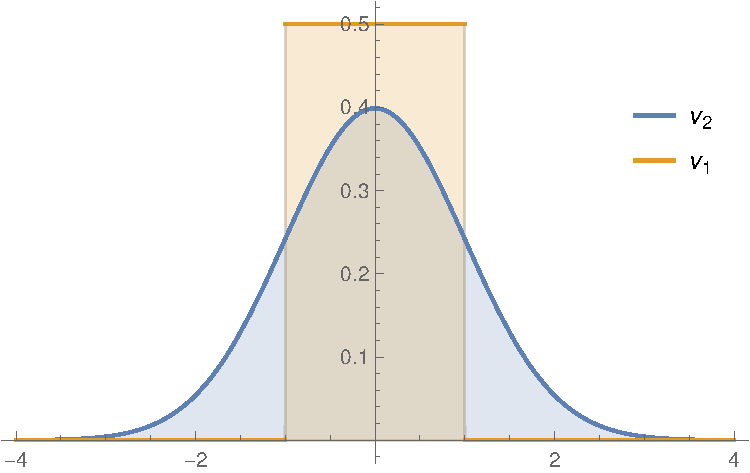
\includegraphics[height=.5\linewidth]{Chapters/OPT_line.pdf}
			\caption{Densities of $\nu_1$ and $\nu_2$}
		\end{minipage}
		\begin{minipage}{.49\textwidth}
			\centering
			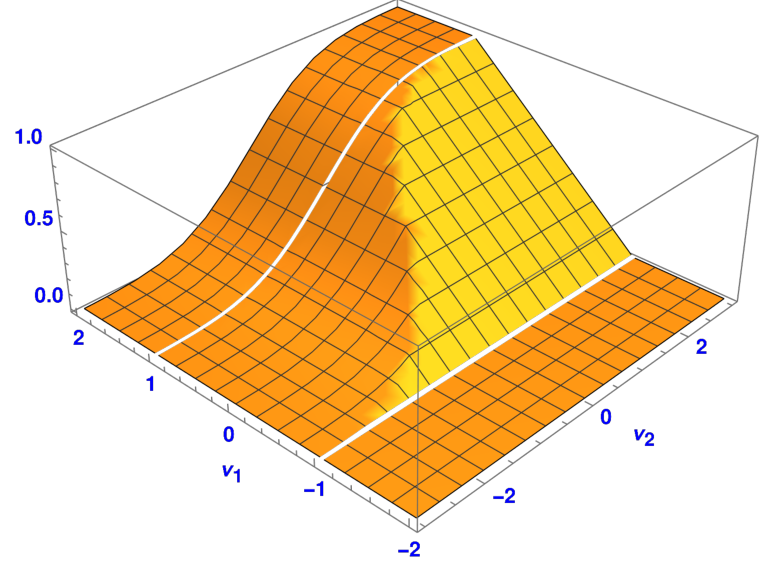
\includegraphics[height=.5\linewidth]{Chapters/cdf_line.pdf}
			\caption{CDF of optimal coupling}
		\end{minipage}
	\end{figure}
	We also draw the cumulative distribution function
	of optimal coupling between $\nu_1$ and $\nu_2$
	by \cite[Theorem 2.18]{villani2003topics}.
	By McCann's displacement interpolation (\cite[Section 5.1.3]{villani2003topics}),
	$\mu =[\frac{1}{2} \operatorname{Id} + \frac{1}{2} \nabla \psi]_{\#} \nu_1$ is the barycenter of $\mathbb{P}$.
	Then the support of $\mu$ could not be compact,
	otherwise the image of transference map is contained
	in a compact set for $\nu_1$ almost everywhere.
\end{rmk}


% \appendix
% %! TEX root = ../barycenter.tex
\chapter{Notes, out of report}
\section{Metric geometry}

The induced length space topology of $(E, \hat{d})$ is not locally compact.
By compatibility of induced length structure (\cite[Exercise 2.1.5]{burago2001course}) with the topology of base space $E$,
open set in original topology $(E, d)$ is again open in the induced length space topology $(E, \hat{d})$.

For non-smooth analysis, we use the definition of speed in \cite[Section 2.7]{burago2001course} for a curve.

\begin{defn}[Speed of curve]
	Let \( ( E , d ) \) be a metric space and \( \gamma : I \rightarrow X \) a curve.
	The speed of \( \gamma \) at \( t \in I \), denoted by \( v _ { \gamma } ( t ) \),
	is defined by
	\[ v _ { \gamma } ( t ) : = \lim _ { \varepsilon \rightarrow 0 } \frac { d ( \gamma ( t ) , \gamma ( t + \varepsilon ) ) } { | \varepsilon | } \]
	if the limit exists.
\end{defn}

We can take arc-length proportional parametrization on $[0,1]$ for any rectifiable curves.
They are then Lipschitz curves, and we recover classic length integral formula.

\begin{thm}
	Let \( E \) be a metric space and \( \gamma : [ a , b ] \rightarrow X \) be a Lipschitz curve.
	Then the speed \( v _ { \gamma } ( t ) \) exists for almost all \( t \in [ a , b ] \) and \( L ( \gamma ) = \)
	\( \int _ { a } ^ { b } v _ { \gamma } ( t ) \diff \lambda \) where $\lambda$ is the Lebesgue measure.
\end{thm}

\begin{rmk}
	Here we should discuss two different length metrics appeared, one is induced from $\ell^2$ norm and the other one is smooth Riemannian length structure. Are they two coincided (on common admissible curves)? Two ways to think about this relation
	\begin{enumerate}
		\item Apply Theorem 2.4.3 in \cite{burago2001course}, we then need to show Riemannian length structure is lower semi-continuous with respect to $\ell^2$ metric.
		\item Consider $E$ as a Hilbert sub-manifold of $\ell^2$, the norm for tangent space is the restriction of canonical norm of $\ell^2$.
	\end{enumerate}
\end{rmk}
\section{Measure theory}

Let \( X \) be a metric space and \( \mathscr { M } ( X ) \) the space of all measures defined on \( \mathscr { B } _ { X } . \) An element \( \mu \in \mathscr { H } ( X ) \) is a nonnegative, countably additive set function defined on \( \mathscr { B } _ { X } \) with the property \( \mu ( X ) = 1 . \quad C ( X ) \) stands for the space of all bounded real valued continuous functions on \( X \). We shall now topologize the space \( \mathscr { M } ( X ) \) by defining a base of open neighborhoods for any point \( \mu . \) Consider the family of sets of the form
\( V _ { \mu } \left( f _ { 1 } , f _ { 2 } , \ldots , f _ { k } ; \varepsilon _ { 1 } , \ldots , \varepsilon _ { k } \right) \)
\[ \left\{\nu \in \mathscr { M } ( X ) \, \mid  \left| \int f _ { i } d v - \int f _ { i } d \mu \right| < \varepsilon _ { i } , \quad i = 1,2 , \ldots , k \right\} \]

where \( f _ { 1 } , f _ { 2 } , \ldots , f _ { k } \) are elements from \( C ( X ) \) and \( \varepsilon _ { 1 } , \varepsilon _ { 2 } , \ldots , \varepsilon _ { k } , \) are positive numbers. It is easy to verify that the family of sets obtained by varying \( k , f _ { 1 } , f _ { 2 } , \ldots , f _ { k } , \varepsilon _ { 1 } , \ldots , \varepsilon _ { k } \) satisfies the axioms of a basis for a topology.

\begin{defn}
	We shall refer to this as the weak topology  in \( \mathscr { M } ( X ) \).
\end{defn}

It is then clear that a net \( \left\{ \mu _ { \alpha } \right\} \) of measures converges in the weak topology to a measure \( \mu \) if and only if \( \int f d \mu _ { \alpha } \rightarrow \int f d \mu \) for every \( f \in C ( X ) . \) In such a case we shall say that \( \mu _ { \alpha } \) converges ``weakly" to \( \mu \) or \( \mu _ { \alpha } \Rightarrow \mu \) in symbols. Unless otherwise stated, \( \mathscr { M } ( X ) \) will always be considered as a topological space with the weak topology.

We shall first recall a theorem which yields several useful equivalent definitions of the weak topology.

\begin{thm}
	Let \( \mu _ { \alpha } \) be a net in \( \mathscr { M } ( X ) . \) Then the following statements are equivalent:
	\begin{itemize}
		\label{thm:weak_convergence}
		\item \( \mu _ { \alpha } \Rightarrow \mu \)
		\item \( \lim _ { \alpha } \int g d \mu _ { \alpha } = \int g d \mu \) for all \( g \in U ( X ) \) where \( U ( X ) \) is the space of all bounded real valued uniformly continuous functions;
		\item \( \overline { \lim } _ { \alpha } \mu _ { \alpha } ( C ) \leqslant \mu ( C ) \) for every closed set \( C \)
		\item \( \lim _ { \alpha } \mu _ { \alpha } ( G ) \geqslant \mu ( G ) \) for every open set \( G \)
		\item \( \lim _ { \alpha } \mu _ { \alpha } ( A ) = \mu ( A ) \) for every Borel set \( A \) whose boundary has \( \mu \) -measure \( 0 . \)
	\end{itemize}
\end{thm}

For each point \( x \in X \) we shall denote by \( p _ { x } \) the measure degenerate at the point \( x \). Denote \( D = \left\{ p _ { x }: x \in X \right\} \).

\begin{lem}
	\label{dirac_measure_weak_homeomorphic}
	\( X \) is homeomorphic to the (topological) subset $D$.
\end{lem}

\begin{proof}
	For any point \( x \) and \( g \in C ( X ) , \) we have \( \int g d p _ { x } = g ( x ) \). If \( x _ { \alpha } \rightarrow x _ { 0 } \) then \( g \left( x _ { \alpha } \right) \rightarrow g \left( x _ { 0 } \right) . \) Hence \( p _ { x _ { \alpha } } \Rightarrow p _ { x _ { 0 } } \). Conversely, let \( p _ { x _ { \alpha } } \Rightarrow p _ { x _ { 0 } } \) If \( x _ { \alpha } \) does not converge to \( x _ { 0 } \), there is an open set \( G \) and a subnet \( \left\{ x _ { \beta } \right\} \) such that \( x _ { 0 } \in G \) and \( x _ { \beta } \in X - G \) for all \( \beta . \) Let \( g \) be a continuous function such that \( 0 \leqslant g \leqslant 1 , g \left( x _ { 0 } \right) = 0 \) and \( g ( x ) = 1 \) for \( x \in X - G \). Then \( \int g d p _ { x _ { \beta } } = 1 , \) while \( \int g d p _ { x _ { 0 } } = 0 . \) This is a contradiction. This completes the proof.
\end{proof}

\begin{lem}
	\( D \) is a sequentially closed subset of \( \mathscr { M } ( X ) \).
\end{lem}

\begin{proof}
	Let \( \left\{ x _ { n } \right\} \) be a sequence of points in \( X \) such that \( p _ { x _ { n } } \Rightarrow q \). Suppose \( \left\{ x _ { n } \right\} \) does not have any convergent subsequence. Then the set \( S = \left\{ x _ { 1 } , x _ { 2 } , \ldots \right\} \) is closed and thus is any subset \( C \) of \( S . \) Since \( p _ { x _ { n } } \Rightarrow q \) we have by Theorem \cref{thm:weak_convergence}, \( q ( C ) \geqslant \overline { \lim } p _ { x _ { n } } ( C ) \) for \( C \subseteq S \). It follows that for every infinite subset \( S _ { 1 } \subseteq S , q \left( S _ { 1 } \right) = 1 \). This is a contradiction since \( q \) is a measure.

	Thus there is a subsequence \( \left\{ x _ { n _ { k } } \right\} , x _ { n _ { k } } \rightarrow x . \) By \cref{dirac_measure_weak_homeomorphic}, \( q = p _ { x } \). Hence \( D \) is sequentially closed.
\end{proof}

\begin{thm}
	\label{finite_support_approximation}
	Let \( X \) be a separable metric space and \( E \subseteq X \) dense in \( X  \). Then the set of all measures whose supports are finite subsets of \( E \) is dense in \( \mathscr{ M } ( X ) \), the set of all Borel probability measures on $X$.
\end{thm}

\begin{proof}
	This proof is copy from Theorem 6.3 in \cite{parthasarathy2005probability}.

	It is obviously enough to prove that the set of all measures whose supports are finite subsets of \( X \) is dense in \( \mathscr { M } ( X ) . \) Let us denote the class of such measures by \( \mathscr { F } ( X ) . \) It is clear that any measure concentrated in a countable subset of \( X \) is a weakly limit of measures from \( \mathscr { F } ( X ) . \) Thus it is sufficient to prove that any measure is a weakly limit of measures vanishing outside countable subsets of \( X \).

	Choose and fix \( \mu \in \mathscr { M } ( X ) \). Since \( X \) is separable we can, for each integer \( n , \) write \( X \) as \( \bigcup _ { j } A _ { n j } , A _ { n j } \cap A _ { n k } = \phi \) if \( j \neq k , A _ { n j } \in \mathscr { B } _ { X } \) for all \( n \) and \( j \) and the diameter of \( A _ { n j } \) is \( \leq 1 / n \) for all \( j \). Let \( x _ { n j } \in A _ { n j } \) be arbitrary. Let \( \mu _ { n } \) be the measure with masses \( \mu \left( A _ { n j } \right) \) at the points \( x _ { n j } , \) respectively. Let $g$ be an arbitrary uniformly continuous (we can even assume Lipchitz continuous here) bounded function, and let \[ \alpha _ { n j } = \inf _ { x \in A _ { n j } } g ( x ) , \quad \beta _ { n j } = \sup _ { x \in A _ { n j } } g ( x ) \]
	Since \( g \) is uniformly continuous and since the diameter of \( A _ { n j } \rightarrow 0 \) as \( n \rightarrow \infty \) uniformly in \( j , \sup _ { j } \left( \beta _ { n j } - \alpha _ { n j } \right) \rightarrow 0 \) as \( n \rightarrow \infty \). Now
	\begin{align*}
		\left| \int g d \mu _ { n } - \int g d \mu \right| & = \left| \sum \int _ { A _ { n j } } \left( g - g \left( x _ { n j } \right) \right) d \mu \right|     \\
		                                                   & \leq \sup_{j} \left( \beta _ { n j } - \alpha _ { n j } \right) \xrightarrow{ n \rightarrow \infty} 0.
	\end{align*}
\end{proof}

\begin{thm}[Prokhorov's theorem]
	If \( \mathcal { X } \) is a Polish space, then a set \( \mathcal { P } \subset P ( \mathcal { X } ) \) is pre-compact for the weak topology if and only if it is tight, i.e. for any \( \varepsilon > 0 \) there is a compact set \( K _ { \varepsilon } \) such that \( \mu \left[ \mathcal { X } \backslash K _ { \varepsilon } \right] \leq \varepsilon \) for all \( \mu \in \mathcal { P } \).
\end{thm}

Later we need to have a measurable selection of barycenter when given measure varies. We refer to Theorem 6.9.6 in \cite{Bogachev2007} for following statement, proof is given as Theorem 35.43 in \cite{kechris1995}.

\begin{thm}
	\label{thm:measurale_selection}
	Let \( X \) and \( Y \) be Polish spaces and let \( \Gamma \in \mathcal { B } ( X \times Y ) \). Suppose, additionally, that the set \( \Gamma _ { x }: = \{ y \in Y: ( x , y ) \in \Gamma \} \) is nonempty and \( \sigma \)-compact for all \( x \in X \). Then \( \Gamma \) contains the graph of some Borel mapping \( f: X \rightarrow Y\).
\end{thm}


\begin{rmk} [Similarity between Wasserstein distance and length structure]
	% This comparison may be used in the discussion of geometric properties of Wasserstein space.
	Following comparison seems mysterious and interesting.
	\begin{itemize}
		\item Wasserstein distance
		      \begin{enumerate}
			      \item lower semi-continuous with respect to weakly convergence
			      \item definition involves infimum
			      \item isometric embedding between base space and Wasserstein space
		      \end{enumerate}
		\item Length structure
		      \begin{enumerate}
			      \item lower semi-continuous with repect to point-wise converge of curves
			      \item definition involves infimum
			      \item isometric embedding between base space and space of geodesics
		      \end{enumerate}
	\end{itemize}
\end{rmk}

\section{Functional analysis}

\begin{thm}[Hahn-Banach Theorem]
	Given two disjoint, nonempty, convex sets $A$ and $B$ in a topological vector space $X$. If \( A \) is compact, \( B \) is closed, and \( X \) is locally convex, then there exist \( \Lambda \in X ^ { * } , \gamma _ { 1 } \in R , \gamma _ { 2 } \in R , \) such that
	\[
		\operatorname { Re } \Lambda x < \gamma _ { 1 } < \gamma _ { 2 } < \operatorname { Re } \Lambda y
	\]
\end{thm}

\begin{thm}[Banach-Alaoglu Theorem]
	% If \( V \) is a neighborhood of 0 in a separable topological vector space \( X , \) and if \( \left\{ \Lambda _ { n } \right\} \) is a sequence in \( X ^ { * } \) such that
	% \[ \left| \Lambda _ { n } x \right| \leq 1 \quad ( x \in V , n = 1,2,3 , \ldots ) \]
	% then there is a subsequence \( \left\{ \Lambda _ { n _ { i } } \right\} \) and there is a \( \Lambda \in X ^ { * } \) such that
	% \[ \Lambda x = \lim _ { i \rightarrow \infty } \Lambda _ { n _ { i } } x \quad ( x \in X ) \]
	If \( V \) is a neighborhood of 0 in a topological vector space \( X \) and if
	\[ K = \left\{ \Lambda \in X ^ { * }: | \Lambda x | \leq 1, \forall x \in V \right\} \]
	then $K$ is weak* compact.
\end{thm}

\begin{rmk}
	\begin{itemize}
		\item Weak convergence of measures coincides with weak* topology on the dual space of bounded continous function $C_b(\mathcal{X})$.
		\item Wasserstein metric toplogy of measures coincides with weak* topology on the (topological) dual space of $(1 + d(x_0, \cdot)^p) C_b(\mathcal{X})$.
		\item $C_b(\mathbb{R})$ is not separable, we can consider the uncountable set of bounded functions taking value $0$ or $1$ on all integers.
		\item The reason why Banach-Alaoglu theorem is not applicable is that the space of measures $P(\mathcal{X})$ is not closed in the weak* topolgy. Otherwise, this space will be weak* compact by Banach-Alaoglu theorem. And since weakly convergence is metriziable, compactness is equivalent to sequential compactness. Then there is a classic counterexample of ``escape of mass". Consider Dirac measures on integers, this set has no accumulation points as measures on $\mathbb{R}$. Tightness is a control on the property of $P(\mathcal{X})$ being closed in weak* topology of the dual of $C_b(\mathcal{X})$.
		\item We can apply Hahn-Banach theorem here:
		      \begin{equation}
			      \label{hahn_banach_application}
			      \mu \in \overline { \operatorname { Conv } } ( \mathcal { K } ) \Longleftrightarrow \mu(f) \leq \sup _ { \nu \in \mathcal { K } } \int _ { \mathcal{X} } f \diff \nu, \quad \forall f \in C _ { b }( \mathcal{X} ).
		      \end{equation}
		      For instance we can prove the separability of \( \mathscr { P } ( \mathcal{X} ) \) by choosing \( \mathcal { K }: = \{ \delta _ { x }: x \in D \} \), where \( D \) is a countable dense subset of \( \mathcal{X}\). By \cref{hahn_banach_application} we easily check that \( \operatorname { Conv } (\mathcal { K }) \subset \mathscr { P } ( \mathcal{X} ) \subset \overline { \operatorname { Conv } } (\mathcal { K } \)) and therefore the subset of all the convex combinations with rational coefficients of \( \delta \)-measures concentrated in \( D \) is weakly dense in \( \mathscr { P } ( \mathcal{X} ) \). The same holds for Wasserstein metric topology.

	\end{itemize}
\end{rmk}

Hence, convex analysis may not help us in the problem of Wasserstein barycenter, as the set of Dirac measures is not convex, not closed in the weak* topology of $C_b(\mathcal{X})$. The main application should optimal transport theory.

\section{Work in progress}

\subsection{Countinous selection of barycenter}

From proof of \cref{thm:barycenter_finite_support_measure},
we can define almost everywhere a
selection of barycenter by barycenter formula \cref{equa:formula_barycenter}
and then extend it by countinuity to a bigger domain.

However,
even the barycenter formula \cref{equa:formula_barycenter} is not defined everywhere.

\subsection{Calculate density function}

Recall that there is no duality between $L^{\infty}(\bar{\mu})$ (possible non-separable) and $L^1 (\bar{\mu})$
in functional analysis even when $M$ is compact with Lebesgue measure.
According to Proposition 4.4.2 in \cite{Bogachev2007} below, we need to show that $\bar{\mu}$ is a linear functional on $L^{\infty}(\bar{\mu})$.
\begin{prop}
	Let \( \mu \) be a finite nonnegative measure.
	A continuous linear function \( \Psi \) on \( L ^ { \infty } ( \mu ) \) has the form
	\( \Psi ( f ) = \int _ { X } f g d \mu \)
	, where \( g \in L ^ { 1 } ( \mu ) \),
	precisely when the set function \( A \mapsto \Psi \left( I _ { A } \right) \) is countably additive.
\end{prop}
We define $\Psi(f):= \int_M f \diff \bar{\mu} = \lim_m \int_M f \diff \bar{\mu}_m$ for $f$ continous.
Extend $\Psi$ to be a continous linear functional on $L^{\infty}(\bar{\mu})$ by Hahn-Banach theorem.
Do we still have $\Psi(I_A) = \bar{\mu}(A)$?

A related discussion is available on
\href{https://math.stackexchange.com/questions/574130/does-weak-convergence-with-uniformly-bounded-densities-imply-absolute-continuity/574888#574888}{math Stack Exchange}.
Think about this example carefully.
Let $\lambda$ be the arglength measure and $\phi_n \ge 0$ a continuous function on $\mathbb T$ with $\int_{\mathbb T} \phi_n\, d\lambda = 1$ and $\phi_n(x) = 0$ if $|x-1| \ge \frac 1n$. Then for each continuous function $f\colon \mathbb T \to \mathbb R$ we have $\int_{\mathbb T} f\phi_n d\lambda \to f(1)$, that is $\phi_n \lambda \to \delta_1$ weakly. But $\delta_1$ is not $\lambda$-continuous.

A digression, generally for question if density of $\bar{\mu}_m$ converges to density of $\bar{\mu}$,
we possibly need asymptotically equicontinuous in \cite{Sweeting1986Converse}.

To attack even more general case,
we should be able to single out a part of $\mathbb{P}$ in the form $\lambda_1 \delta_{\mu_1}$
with lower bound on $\lambda_1$ and dominated $\mu_1$.
One way to do so is to assume $\mu_1$ has bounded density.
\begin{defn}
	[The set $ \mathcal { A } _ { L }$]
	For \( 0 < L < \infty \), let \( \mathcal { A } _ { L } \subset W_2(M) \) be the set of Borel probability
	measures with compact support on \( M \), absolutely continuous with respect to volume, whose densities have \( L ^ { \infty } \)
	norm less than or equal to \( L\).
\end{defn}

Note that, since the bound on the \( L ^ { \infty } \) norm is preserved under weak-* convergence,
\( \mathcal { A } _ { L } \) is a countable union of weakly-* closed set, and thus Borel measurable, subset of \( W_2( M ) \).

% If $\mu_1 \in \mathcal{A}_L$, then by duality between $L^p(\bar{\mu})$ and $L^q(\bar{\mu})$
% and that they are separable spaces,
% we have that $\bar{\mu}$ has density in $L^p(\bar{\mu})$ for
% $p < \infty$ with a upper norm bound depending only on constat $L$ (, $\lambda_1$ and $M$).
% We pass $p$ to infity to get $\bar{\mu} \in \mathcal{A}_L$.
% Hence, our conclusion holds for any $\mathbb{P}$ that is not atomless on $\mathcal{A}_L$.

Finally, if we are given $\mathbb{P}$ with only assumption that $\mathbb{P}(\mathcal{A}_L(M)) > 0$,
we need more control on the density function of $\bar{\mu}_m$
to ``remove'' the dependency of its upper bound on a singled-out coefficient $\lambda_1$.
One hope is that $\lambda_1$ is replaced by $\mathbb{P}(\mathcal{A}_L(M))$.


Every measure $\mu$ on $M$ in following discussion is absolutely continous and has compact support.
Here we use the fact that all possible values of $B(x_1, \ldots, x_n)$ are contained in a bounded set if each $x_i$ varies in a bounded set.
To conculde it, since $f$ is continous, there is a upper bound of $f$ and thus a upper bound of distance between $x_i$ and $B(x_1, \ldots, x_n)$.
% We always apply continuities of tranfer maps to get compact support of barycenter measure.
By convention, we denote by $g$ the density function for absolutely measure $\mu$.
One principle of differential geometry is to differentiate everything once we could.

% If we only apply general bound on $c$-concave function
Recall change of variable in \cref{thm:jacobian_identity} (Theorem 4.2 in \cite{cordero2001riemannian}),
\[
	\bar{g} = g_i \circ T_i \det D T_i :
	= g_i \circ T_i \det[Y(H-\text{Hess} u_i)]
\]
where $T_i = \exp(-\nabla u_i)$ is the unique optimal maps from $\bar{\mu}$ to $\mu_i$.
Note that this is why we need that all measures have compact support.

For general $c$-concave function $\mu_i$, we have only upper hessian bound.
And this is not enough to get an estimation on the absolute value of Jacobian determinants.
% For instance, in Euclidean space, $DT_i = (\lambda_i -1)/\lambda_i \leq \text{Id}$.


There is only one element $\gamma$ in the set $\Gamma$ by uniqueness of optimal plans
since coupling between $\bar{\mu}$ and $\mu_i$ is optimal.
% We can get every $\mu_i$ from $\mu_1$ if first push $\mu_1$ to $\bar{\mu}$ through $T_1^{-1}$ then push $\bar{\mu}$ to $\mu_i$ through $T_i$. Hence,
% \[B \circ (T_1, T_2, \ldots, T_n) \circ T_1^{-1} = T_1^{-1}\]
% is the unique transfer map from $\mu_1$ to $\bar{\mu}$. That is to say, $\bar{\mu}$-a.e., $B \circ (T_1, T_2, \ldots, T_n) $ is the identity map.
Hence, $\gamma = (T_1, T_2, \ldots, T_n)_{\#}\bar{\mu}$
	is concentrated on the image of $(T_1, T_2, \ldots, T_n)$.
We have $B_{\#}(T_1, T_2, \ldots, T_n)_{\#}\bar{\mu}=\bar{\mu}$,
thus $B(T_1, T_2, \ldots, T_n) = \text{Id}$ for $\bar{\mu}$ almost everywhere
by uniqueness of optimal plans from $\bar{\mu}$ to $\bar{\mu}$.
This is already included in \cref{lem:inverse_barycenter}.
We differentiate the equality $B(T_1(x), \ldots, T_n(x))=x$ for $\bar{\mu}$-a.e. $x$,
\begin{align*}
	\text{Id} =\sum_{i=1}^n \partial_i B\, DT_i
	 & =\sum_{i=1}^n D \exp(-\frac{1}{\lambda_i}\nabla f_i) \, D \exp(-\nabla u_i)                     \\
	 & =\sum_{i=1}^n D \exp^{-1}(-\nabla \left( \frac{f_i}{\lambda_i}\right)^c) \, D \exp(-\nabla u_i) \\
	 & =\sum_{i=1}^n(H-\text{Hess}(f_i / \lambda_i)^c)^{-1}\,Y_i^{-1}\,
	Y_i\,(H-\text{Hess} u_i)                                                                           \\
	 & =\sum_{i=1}^n(H-\text{Hess}(f_i / \lambda_i)^c)^{-1}\,
	(H-\text{Hess}u_i) .
\end{align*}

Then by Minkowski's determinant inequality, we get
\begin{align*}
	1 & \geq \sum_{i=1}^{n} \det [H-\text{Hess}(f_i/\lambda_i)^c]^{-1/n}\,\det[H-\text{Hess}u_i]^{1/n} \\
	  & =\sum_{i=1}^n \det[\partial_i B]^{1/n}\,\det[DT_i]^{1/n}
\end{align*}
Observe that in our discussion $(f_i / \lambda_i)^c$ is calculated at the barycenter $x$ of $\sum_{j=1}^{n} \delta_{T_j x}$,
and patial derivative means all $T_j x$ for $ j \ne i$ are fixed in calculation.
Hence, we can have $(f_i / \lambda_i)^c = g_i$.
% Recall that we know $(f_i / \lambda_i)^c$ has hessian bound from both sides, see \cref{equa:hessian_bound_f}.
From it we get $\det[\partial_i B]^{1/n} \geq \min \{1, \lambda_i / (1 - \lambda_i)\} > \lambda_i$,
where $C > 0$ depends only on hessian bound of square distance function and Lipschitz constant of exponential map.

Combine these two inequalities, and we then apply Jensen inequlity
\[
	\bar{g} \leq
	\left[ \sum_{i=1}^n \frac{\det[\partial_i B]^{1/n}}
	{g_i^{1/n} \circ T_i}\right]^{-n}
	< \left[ \sum_{i=1}^n \frac{C \, \lambda_i}
	{g_i^{1/n} \circ T_i}\right]^{-n}
	\leq C^{-n} \sum_{i=1}^n \lambda_i g_i \circ T_i.
\]
With this estimation in hand,
one shows easily that if measure $\mathbb{P} \in \mathcal{W}_2(\mathcal{W}_2(M))$ on $W_2(M)$ give mass to the measurable set $\mathcal{A}_L$,
then it has a unique absolutely continous barycenter.

\subsubsection{Jacobian determinant inequality for the Wasserstein barycenter}

This is done by Kim and Pass.
\begin{defn}[Volume distortion]
	Let \( \lambda \) be a Borel probability measure on \( M \) with a
	unique barycenter \( \bar { x } \) (that is, such that \( B C ( \lambda ) \) is a singleton). We define the generalized,
	or barycentric, volume distortion coefficients at \( y \notin \operatorname { cut } ( \bar { x } ) \)

	\[ \alpha _ { \lambda } ( y ) : = \frac { \operatorname { det } \left[ - \left. D _ { y z } ^ { 2 } \right| _ { z = \bar { x } } c ( y , z ) \right] } { \operatorname { det } \left[ \left. \int _ { M } D _ { z z } ^ { 2 } \right| _ { z = \bar { x } } c ( x , z ) d \lambda ( x ) \right] } \]
	where \( D _ { z z } ^ { 2 } c ( x , z ) \) denotes the Hessian of the function \( z \mapsto c ( x , z ) \), and the determinants
	are computed in exponential local coordinates at \( \bar { x } \) and \( y . \)
\end{defn}

\begin{thm}
	[Jacobian determinant inequality for the Wasserstein barycenter]
	Assume that the Wasserstein barycenter \( \bar { \mu } \) of the measure \( \Omega \) on \( P ( M ) \) is absolutely continuous.
	Letting \( T _ { \mu } \) denote the optimal map from \( \bar { \mu } \) to \( \mu \), consider the measure on \( M \) given by
	\[ \lambda _ { x } : = \int _ { P ( M ) } \delta _ { T _ { \mu } ( x ) } d \Omega ( \mu ) \]
	which is defined with respect to a.e. $x$.
	Then, for \( \bar { \mu } \)-a.e. \(x\),
	\[ 1 \geq \int _ { P ( M ) } \alpha _ { \lambda _ { x } } ^ { 1 / n } \left( T _ { \mu } ( x ) \right) \operatorname { det } ^ { 1 / n } D T _ { \mu } ( x ) d \Omega ( \mu ) \]
\end{thm}

% \subsubsection{Use local coordinate}
% Need to work on it.

\subsubsection{Use Skorohod representation}
\textcolor{red}{This is not possible!}
One may consider to construct absolutely continous random variables.
For example, to use the Skorohod representation (see section 8.5 in \cite{Bogachev2007}),
\begin{defn}
	We shall say that a topological space \( X \) has the strong
	Skorohod property for Radon measures if to every Radon probability measure
	\( \mu \) on \( X \),
	one can associate a Borel mapping \( \xi _ { \mu } : [ 0,1 ] \rightarrow X \) such that \( \mu \) is
	the image of Lebesgue measure under the mapping \( \xi _ { \mu } \) and \( \xi _ { \mu _ { n } } ( t ) \rightarrow \xi _ { \mu } ( t ) \) a.e.
	whenever the measures \( \mu _ { n } \) converge weakly to \( \mu . \)
\end{defn}

However, even if $\mu$ is absolutely continous respect to Lebesgue measure on $\mathbb{R}$,
we don't have necessarily that $\xi_{\mu}$ is a absolutely continous function.
In fact, the Housdorff dimension of the image of $\xi_{\mu}$ is not likely to be greater than 2.
See \cite{Besicov1937Sets} for discussions on $\delta$-Lipschitz curves,
their Housdorff dimensions are bounded by $2-\delta$.

% \subsection{Control on density function}

% %! TEX root = ../barycenter.tex
\chapter{Paper review}
\section{Barycenters in Alexandrov spaces of curvature bounded below}
Then we discuss the infinitesimal structure of an Alexandrov space \( ( X , d )\).

\begin{rmk}[Example 2.1 c]
	% This example is in contradiction with \href{https://en.wikipedia.org/wiki/Hadamard_space}{Wikipedia: Hadamard space}. The author claims Hilbert space is of non-negative curvature, while Wikipedia says ``a normed space is an Hadamard space if and only if it is a Hilbert space".
	Hilbert space satisfies equality in triangle comparison with Euclidean space, hence can be regarded ``flat".
\end{rmk}
\begin{defn}[space of directions]
	Fix \( z \in X \) and let \( \hat { \Sigma } _ { z } \) be the set of all unit speed geodesics emanating from \( z \). For \( \gamma , \eta \in \hat { \Sigma } _ { z } , \) by virtue of the curvature bound, the limit
	\begin{equation}
		\label{angle_def}
		\angle _ { z } ( \gamma , \eta ): = \arccos \left( \lim _ { s , t \downarrow 0 } \frac { s ^ { 2 } + t ^ { 2 } - d _ { X }\left( \gamma ( s ) , \eta ( t ) \right) ^ { 2 } } { 2 s t } \right)
	\end{equation}
	exists and is regarded as the angle (pseudo-)distance of \( \hat { \Sigma } _ { z } . \) We define the space of directions \( \left( \Sigma _ { z } , \angle _ { z } \right) \) at \( z \) as the completion of \( \Sigma _ { z } / \sim \) with respect to \( \angle _ { z } , \) where \( \gamma \sim \eta \) if \( \angle _ { z } ( \gamma , \eta ) = 0 . \)
\end{defn}

\begin{defn}[tangent cone]
	The tangent cone \( \left( C _ { z } , d _ { C _ { z } } \right) \) is defined as the Euclidean cone over \( \left( \Sigma _ { z } , \angle _ { z } \right) , \)
	that is to say,
	\begin{align*}
		C _ { z }:                                           & = \Sigma _ { z } \times [ 0 , \infty ) / \Sigma _ { z } \times \{ 0 \}          \\
		d _ { C _ { z } } ( ( \gamma , s ) , ( \eta , t ) ): & = \sqrt { s ^ { 2 } + t ^ { 2 } - 2 s t \cos \angle _ { z } ( \gamma , \eta ) }
	\end{align*}
\end{defn}

\begin{thm}[Computation of distance in tangent cone]
	Let $\gamma$ and  $\eta$ be two geodesics from unit interval into $X$ starting at $z$. Then $\gamma^\prime(0)$ and $\eta^\prime(0)$ are naturally elements in $C_z$. We can calculate their distance as:
	\[  d_{C_z}(\gamma^\prime(0),\eta^\prime(0))=\lim _ { t \downarrow 0 } \frac  {d ( \eta ( t ) , \gamma ( t ) )  }{ t }\]
\end{thm}

\begin{proof}
	This is a calculation of angle between $\gamma^\prime(0)$ and $\eta^\prime(0)$ with a specific selected converging process. To apply angle definition in \Cref{angle_def}, normalize $\gamma$ and $\eta$ as $\gamma\left(\vert\gamma^\prime(0)\vert \cdot\right)$ and $\eta\left(\vert\eta^\prime(0)\vert \cdot\right)$
	\[
		\cos\angle _ { z } ( \gamma , \eta ): = \left( \lim _ { s , t \downarrow 0 } \frac { s ^ { 2 } + t ^ { 2 } - d _ { X }\left( \gamma (\vert \gamma^\prime(0)\vert s ) , \eta (\vert \eta^\prime(0)\vert  t ) \right) ^ { 2 } } { 2 s t } \right)
	\]
	To get desired formula, put $ x := \vert  \gamma^\prime(0)\vert s =\vert \eta^\prime(0)\vert t $ and pass $x \downarrow 0$.
\end{proof}

\begin{rmk}[Lemma 4.5, Lang and Schroeder's inequality]
	When passing from finite support measures to general ones, the author should use Wasserstein metric $W_p$ convergence but not only weak convergence. Otherwise, he cannot justify convergence of integrals of distance function $d_{C_z}$. Here we use the fact that finite supported measures is a dense subspace of Wasserstein space $\mathcal{W}_2(X)$ if $X$ is a Polish space (see \cite{villani2008optimal} Theorem 6.18), recalled in this report as \Cref{thm:topology_Wasserstein}.
\end{rmk}

\section{Paper review for Kim and Pass}

This is review of \cite{KIM2017640},
Wasserstein barycenters over Riemannian manifolds.

\subsection{Remind of basics in Riemannian geometry}

For \( c ( x , y ) = \frac{ 1 } { 2 } d ^ { 2 } ( x , y ) \), to show \( - D _ { x } c ( x , y ) = \exp _ { x } ^ { - 1 } ( y ) \), we should use exponetial coordinate at $T_yM$.
By Gauss lemma, we have \( \nabla r = \partial _ { r } \).
As $d c = r dr$, $\nabla c = r \partial r$ and our conculsion follows from that $ r \partial r $ is of length $r$.

It is instructive to recall proof of Gauss lemma in \cite{Petersen2016}.
On \( U = \exp _ { p } ( B ( 0 , \varepsilon ) ) \) we define the function \( r ( x ) = \left| \exp _ { p } ^ { - 1 } ( x ) \right| . \)
That is, \( r \) is simply the Euclidean distance function from the origin on \( B ( 0 , \varepsilon ) \subset T _ { p } M \) in exponential coordinates.
This function can be continuously extended to \( U \) by defining \( r ( \partial U ) = \varepsilon . \)

We know that \( \nabla r = \partial _ { r } = \frac { 1 } { r } x ^ { i } \partial _ { i } \) in Cartesian coordinates
on \( T _ { p } M . \)
We show that this is also the gradient with respect to the general metric \( g . \)

\begin{lem}
	[The Gauss Lemma]
	On \( ( U , g ) \) the function \( r \) has gradient \( \nabla r = \partial _ { r } \), where \( \partial _ { r } = D \exp _ { p } \left( \partial _ { r } \right) \).
\end{lem}

\begin{proof}
	We select an orthonormal basis for \( T _ { p } M \) and introduce
	Cartesian coordinates.
	These coordinates are then also used on \( U \) via the exponential map.
	Denote these coordinates by \( \left( x ^ { 1 } , \ldots , x ^ { n } \right) \) and the coordinate vector fields by
	\( \partial _ { 1 } , \ldots , \partial _ { n } . \)
	Then
	\begin{align*}
		r ^ { 2 }        & = \left( x ^ { 1 } \right) ^ { 2 } + \cdots + \left( x ^ { n } \right) ^ { 2 } , \\
		\partial _ { r } & = \frac { 1 } { r } x ^ { i } \partial _ { i }.
	\end{align*}
	For this, take a function $f: M \mapsto \mathbb{R}$, we have $ \frac{\partial f}{\partial x_i}=\frac{\partial f}{\partial r}\cdot \frac{\partial r}{\partial x_i}$.
	Differentiate $ r ^ { 2 } = \left( x ^ { 1 } \right) ^ { 2 } + \cdots + \left( x ^ { n } \right) ^ { 2 } $, we get $\frac{\partial r}{\partial x_i} = \frac{x_i}{r} $.
	Apply this equality agian, we can solve $\frac{\partial f}{\partial r}$ from $\frac{\partial f}{\partial x_i}$.

	To show that this is the gradient field for \( r ( x ) \) on \( ( M , g ) \), we must prove that \( d r ( v ) = \)
	\( g \left( \partial _ { r } , v \right) . \)
	We already know that
	\[
		d r = \frac { 1 } { r } \left( x ^ { 1 } d x ^ { 1 } + \cdots + x ^ { n } d x ^ { n } \right),
	\]
	but have no knowledge of $g$, since it is just some abstract metric.

	One can show that \( d r ( v ) = g \left( \partial _ { r } , v \right) \) by using suitable Jacobi fields for \( r \) in place of \( v \). Let us start with \( v = \partial _ { r } . \)
	The right-hand side is 1 as the integral curves for \( \partial _ { r } \) are unit speed geodesics.
	The left-hand side can be computed directly and is also $1$.
	Next, take a rotational field \( J = - x ^ { i } \partial _ { j } + x ^ { j } \partial _ { i } , i , j = 1 , \ldots , n , i < j . \)
	In dimension $2$ this is simply the angular field \( \partial _ { \theta } \).
	An immediate calculation shows that the left-hand side vanishes: \( d r ( J ) = 0 \).
	For the right-hand side we first note that \( J \) really is a Jacobi field as \( L _ { \partial _ { r } } J = \left[ \partial _ { r } , J \right] = 0 . \)
	Using that \( \nabla _ { \partial _ { r } } \partial _ { r } = 0 \) we obtain
	\[ \begin{aligned}
			\partial _ { r } g \left( \partial _ { r } , J \right) & = g \left( \nabla _ { \partial _ { r } } \partial _ { r } , J \right) + g \left( \partial _ { r } , \nabla _ { \partial _ { r } } J \right) \\
			                                                       & = 0 + g \left( \partial _ { r } , \nabla _ { \partial _ { r } } J \right)                                                                   \\
			                                                       & = g \left( \partial _ { r } , \nabla _ { J } \partial _ { r } \right)                                                                       \\
			                                                       & = \frac { 1 } { 2 } D _ { J } g \left( \partial _ { r } , \partial _ { r } \right)                                                          \\
			                                                       & = 0
		\end{aligned} \]
	Thus \( g \left( \partial _ { r } , J \right) \) is constant along geodesics emanating from \( p \).
	To show that it vanishes first observe that
	\[ \begin{aligned} \left| g \left( \partial _ { r } , J \right) \right| & \leq \left| \partial _ { r } \right| | J |                                                                               \\
                                                                     & = | J |                                                                                                                  \\
                                                                     & \leq \left| x ^ { i } \right| \left| \partial _ { j } \right| + \left| x ^ { j } \right| \left| \partial _ { i } \right| \\
                                                                     & \leq r ( x ) \left( \left| \partial _ { i } \right| + \left| \partial _ { j } \right| \right)\end{aligned} \]
	Continuity of \( D \exp _ { p } \) shows that \( \partial _ { i } , \partial _ { j } \) are bounded near \( p .  \)
	Thus \( \left| g \left( \partial _ { r } , J \right) \right| \rightarrow 0 \) as \( r \rightarrow 0 .  \)
	This forces \( g \left( \partial _ { r } , J \right) = 0 .\)
	Finally, observe that any vector \( v \) is a linear combination of \( \partial _ { r } \) and rotational fields.
	This proves the claim.
\end{proof}

\subsection{Fix typos and correct statements}

We copy original statement and put reference number directly after it.

\begin{rmk}[Remark 2.2]
	Inspection of the proof above shows that \( ( M \), vol \( ) \) can be replaced with a \cancel{compact separable} metric space \( ( X , \nu ) \) equipped with a reference Borel measure \( \nu \).
\end{rmk}

We only need an outer regular reference measure. And Borel measure on metric space is regular, see Theorem 7.1.7 in \cite{Bogachev2007}.

\begin{prop}[Proposition 2.9 Distortion under Ric \( \geq 0 \)]
	Suppose the Ricci curvature of \( M \) is everywhere nonnegative, i.e., Ric \( \geq 0 . \) Then, for any \( x \in M \) and \( \lambda \in P ( M ) \), \textcolor{blue}{if $\lambda$ gives no mass to the cut-locus of its baryceter $\widebar{x}$}, we have
	\[ \alpha _ { \lambda } ( x ) \geq 1 \]
\end{prop}

\begin{proof}[Proof of Prop 2.9]
	Minimality of \( z \mapsto \int _ { M } c ( x , z ) \diff \lambda ( x ) \) at the barycenter \( \widebar { x } \), combined with semi-concavity of \( z \mapsto c ( x , z ) \) and Fatou's lemma yields
	\[
		\int _ { M } \left. D _ { z z } ^ { 2 } \right| _ { z = \widebar { x } } c ( x , z ) \diff \lambda ( x ) \geq 0
	\] as a matrix.
\end{proof}

Locally $c(x,z)=:d^2_x(z)$ near $\widebar{x}$ is a geodesically convex function, by linear intergration so is the integral  \( z \mapsto \int _ { M } d^2_x(z) \diff \lambda ( x ) \).
As convexity implies local Lipschitz, $d^2_x(z)$ is also differentiable near $\widebar{x}$ and so is its integral by compactness of $M$.
Thus we have locally for $\lambda$-almost all $x$ (not in the cut-locus of $\widebar{x}$, arguing with semi-concavity is not strong as this),
% \textcolor{red}{why differentiability of $d^2_x(z)$ implies smoothness?}
\begin{equation}
	\label{equa:convex_distance_inequality}
	d^2_x \left( \exp _ {\widebar{x}} u \right) - d^2_x (\widebar{x}) - \langle \nabla d^2_x (\bar{x}) , u \rangle = \frac { 1 } { 2 } \langle \left. D _ { z z } ^ { 2 } \right| _ { z = \bar { x } } d^2_x(z) \, u , u \rangle + o \left( | u | ^ { 2 } \right) > 0
\end{equation}

To show positivity of matrix, we take a vector $\nu$ and set $\mu = h \nu$ with $h > 0$ small enough.
Divide by $h$ in \cref{equa:convex_distance_inequality} and then take integral,
\[
	\langle \left. D _ { z z } ^ { 2 } \right| _ { z = \widebar { x } } \int_{M} d^2_x(z) \diff \lambda ( x )\, v , v \rangle + \frac{o (h^2)}{h^2} = \int_{M} \langle \left. D _ { z z } ^ { 2 } \right| _ { z = \widebar { x } } d^2_x(z)\, v , v \rangle + \frac{o (h^2)}{h^2} \diff \lambda ( x ).
\]
Note that here we need compactness of $M$, hence boundness of $ \nabla d^2_x(\widebar{x}) $ for $x \in M$, to get inter-change of integral and gradient:
\[
	\int_M \langle \nabla d^2_x (\widebar{x}) , u \rangle \diff \lambda (x) = \langle \int_M \nabla d^2_x (\widebar{x}) \diff \lambda (x) , u \rangle
\]
Apply Fatou's lemma, let $f\downarrow 0$,
\[
	\langle \left. D _ { z z } ^ { 2 } \right| _ { z = \widebar { x } } \int_{M} d^2_x(z) \diff \lambda ( x )\, v , v \rangle \leq \langle \int_{M} \left. D _ { z z } ^ { 2 } \right| _ { z = \widebar { x } } d^2_x(z) \diff \lambda(x)\, v, v \rangle.
\]
And by minimallity of $\widebar{x}$, we know left hand side is non-negative.

This argument is also used in Prop 4.2.

\begin{rmk}[Remark 3.2]
	... In fact, it holds for any (compact) metric
	space on which the optimal \cancel{maps} \textcolor{blue}{plans}, \( T _ { \# } \mu = \nu \), exist uniquely for any arbitrary absolutely continuous source measure \( \mu \).
\end{rmk}

\begin{lem}[Lemma  4.1  a.e. \( x \) and $ \Omega$-a.e. $\mu$ ]
	Let \( \widebar { \mu } \in \cancel{P ( M )} \textcolor{blue}{P_{ac}(M)}\) and for each \( \mu \in P ( M ) \), let \( u _ { \mu } \) be the dual potential (whose gradient is uniquely determined \( \widebar { \mu } \) almost everywhere) for the optimal transport problem between \( \bar { \mu } \) and \( \mu . \) Let \( \Omega \) be a Borel probability on \( P ( M ) . \) For volume almost all \( x , x \mapsto u _ { \mu } ( x ) \) is twice differentiable for \( \Omega \) -almost all \( \mu \in P ( M ) . \)
\end{lem}

\begin{proof}
	$\forall \mu, x \mapsto \mu_u(x)$ is twice differentiable for $\widebar{\mu}$-a.e. $x$. Apply Fubini's theorem then.
\end{proof}

\begin{prop} [Prop 4.2 Derivatives inside the integral $\int _ { P ( M ) } \diff \Omega$]
	\begin{equation}
		\label{equa:first_order}
		\nabla _ { x } \int _ { P ( M ) } u _ { \mu } ( x ) \diff \Omega ( \mu ) = \int _ { P ( M ) } \nabla _ { x } u _ { \mu } ( x ) \diff \Omega ( \mu )
	\end{equation}
	\begin{equation}
		\label{equa:second_order}
		\nabla _ { x } ^ { 2 } \int _ { P ( M ) } u _ { \mu } ( x ) \diff \Omega ( \mu ) \geq \int _ { P ( M ) } \nabla _ { x } ^ { 2 } u _ { \mu } ( x ) \diff \Omega ( \mu )
	\end{equation}
\end{prop}

\begin{proof}
	This can be seen by applying the dominated convergence theorem for \cref{equa:first_order} due to uniform Lipschitzness \textcolor{blue}{by \cref{lem:infimal_convolution_Lipschitz}} of \( u _ { \mu } \) and Fatou's lemma for \cref{equa:second_order} due to the semi-convexity
	of \( u _ { \mu } . \)
\end{proof}

% This shouldn't be an independent proposition, rather we can only condsider it in the case of Theorem 4.4.
% $u_{\mu}$ is uniformly Lipschitz on $x\in M$, this shows that $\nabla_{x}u_{\mu}$ is finite but not necessarily bounded (dominated).
To get rid of measurable selection problem, we consider
\[ y \mapsto \int_{P(M)} c(y, T_{\mu}(x)) \diff \Omega ( \mu)\]
at point $x$.
Here we assume $\widebar{\mu}$ is barycenter of $\Omega$ and $T_{\mu}$ is the transfer map from $\widebar{\mu}$ to $\mu$.
Then this integral valued map is well-defined $\mu$-a.e. by Fubini's theorem.
By stability of Kantorobich potentials (Theorem 1.52 in \cite{Santambrogio2015}), $c(y, T_{\mu}(x))$ is continous with respect to $\mu \in P(M)$.
Fix a $\mu$, $c(y, T_{\mu}(x))$ is locally Lipschitz with respect to $y$.
By continuity Lipschitz inequality will hold as well in a neighbourhood of $\mu$.
Consider these local neighbourhoods cover on compact set $ M \times P(M)$,
we can then get a uniform boundness on
\[\left. D_y\right|_{y=x} c(y, T_{\mu}(x)) = - \nabla_x u_{\mu}(x).\]

\begin{lem} [Lem 4.3 Riemannian barycenter from Wasserstein barycenter]
	\label{lem:inverse_barycenter}
	Let \( \widebar { \mu } \) be a Wasserstein barycenter of the measure \( \Omega \) on \( P ( M ) \) and assume \( \widebar { \mu } \) is absolutely continuous with respect to volume;
	let \( T _ { \mu } \) be an optimal map from \( \widebar { \mu } \) to \( \mu . \)
	Let \( \lambda _ { z } = \left( \mu \mapsto T _ { \mu } ( z ) \right) _ { \# } \Omega . \)
	Then, for \( \widebar { \mu } \) almost every \( z , z \) is a barycenter of \( \lambda _ { z }\).
	\textcolor{blue}{And $\lambda_z$ gives no mass to the cut-locus of $z$} by \Cref{prop:differentiate_optimal_transport}.

	If, in addition, \( \Omega \left( P _ { a c } ( M ) \right) > 0 \), then for \( \widebar { \mu } \) almost every \( z , z \) is the unique barycenter of $\lambda _ { z }$.

\end{lem}

There is an explanation behind this lemma. Consider we have random images, and we want to approch a best representative of them by simulation. We process this by compose all barycenters of simulated images into an average image. On the other hand, for each grid point in our average image, we can simulate a new image by transfering that grid point optimally. This lemma claims that that choosen grid point should be a barycenter of the new generated image. This could be related to ergodic theory as there are two kinds of averages involved.

\begin{proof}[Proof of the 1st order balance]
	...
	% On the other hand, by Lemma  4.3, for \( \widebar { \mu } \) almost every \( x \), we have that \( x \) is the
	% barycenter of \( \lambda _ { z } = \left( \mu \mapsto T _ { \mu } ( z ) \right) _ { \# } \Omega ; \) that is, a minimizer of
	% \[ f _ { x } : y \mapsto \int _ { P ( M ) } d ^ { 2 } \left( y , T _ { \mu } ( x ) \right) d \Omega ( \mu ) .\]

	Therefore, the latter function \( f _ { x } \), which is semi-concave is differentiable at \( x : \) due to semi-concavity, there is \( C > 0 \) such that the function \( f _ { x } ( y ) - C \operatorname { dist } ^ { 2 } ( x , y ) \) is locally geodesically concave near \( x \).
	Minimality at \( x \) implies \( f _ { x } ( y ) - C \operatorname { dist } ^ { 2 } ( x , y ) \geq f _ { x } ( x ) - \) \( C \operatorname { dist } ^ { 2 } ( x , \cancel{x}\, \textcolor{blue}{y} ) \).
	Since \( y \mapsto f _ { x } ( x ) - C \operatorname { dist } ^ { 2 } ( x , y ) \) has vanishing derivative at \( x \), concavity of \( f _ { x } ( y ) - C \operatorname { dist } ^ { 2 } ( x , y ) \) implies that locally the function \( y \mapsto f _ { x } ( y ) - C \operatorname { dist } ^ { 2 } ( x , y ) \) is also
	locally bounded from above by the constant \( f _ { x } ( x ) . \) This implies the differentiability of
	\( f _ { x } \) at \( x \).
\end{proof}

% \textcolor{cyan}{If we have} that $\lambda_{z}$ is absolutely continous, then we prove first order balance by taking gradient under integral.
% For the sencond paragraph of argument,
To simplify, we should prove:
\begin{lem}
	For $f, g$ two convex functions near $0$, assume $f(0)=g(0)=g^\prime(0)=0$. If $f \leq g$ and $0$ is a local minimum of $g$, we then have $f \geq 0$ and $f$ is differentiable at $0$.
\end{lem}

\begin{proof}
	We need to show that subdifferential $\partial f(0) $ of $f$ is a single point set $ \{ 0 \}$. $\forall u \in \partial f( 0 )$,
	\[
		\langle x, u \rangle \leq f(x) - f(0) = f(x) \leq g(x) = g(x) - g(0),
	\]
	that is say, $ u \in \partial g(0)$. Hence $ \partial f(0) = \partial g(0) = \{0\}$.

\end{proof}

\begin{proof}[Proof of Theorem 4.6]
	...\\
	Note that each \( - D _ { x y } ^ { 2 } c \left( x , T _ { \mu } ( x ) \right) D T _ { \mu } ( x ) = D _ { x x } ^ { 2 } u _ { \mu } ( x ) + D _ { x x } ^ { 2 } c \left( x , T _ { \mu } ( x ) \right) \) is positive semi-definite by the \( c \)-convexity of \( u _ { \mu } \), and hence so is their integral...
\end{proof}

By definition, we have
\[
	\inf_{\textcolor{cyan}{z}} u_\mu(\textcolor{green}{z}) + c(\textcolor{green}{z}, T_\mu(x))= u_\mu(x) + c(x, T_\mu(x)) = - u^c ( T_\mu(x)).
\]
If consider derivative with respect to first variable,
then we have first differential vanishes and Hessian semi-positive.

% \section{Multi-marginal optimal transport on Riemannian manifolds}
% We will prove uniqueness and Monge solution results for the multi-marginal problem on a compact Riemannian manifold,
% with cost function
% \begin{equation}
% 	\label{equa:mult-imarginal_problem}
% 	c \left( x _ { 1 } , x _ { 2 } , \ldots , x _ { m } \right) = \inf _ { y \in M } \sum _ { i = 1 } ^ { m } \frac { d ^ { 2 } } { 2 } \left( x _ { i } , y \right)
% \end{equation}

% \begin{lem}
% 	The cost function \( c \) is everywhere superdifferentiable with respect to \( x _ { 1 } \).
% 	That is, for all \( \left( x _ { 1 } , x _ { 2 } , \ldots , x _ { m } \right) \in M ^ { m } \) there exist \( p \in T _ { x _ { 1 } } M \) (the super-gradient) such that, for small \( v \in T _ { x _ { 1 } } M \), we have
% 	\[ c \left( \exp _ { x _ { 1 } } v , x _ { 2 } , \ldots , x _ { m } \right) \leq c \left( x _ { 1 } , x _ { 2 } , \ldots , x _ { m } \right) + g ( p , v ) + o ( | v | ) \]
% \end{lem}

% \begin{lem}
% 	At any point \( \left( x _ { 1 } , \ldots , x _ { m } \right) \) where \( c \) is differentiable with respect to
% 	\( x _ { 1 } \), there is a unique minimizing \( y \) in \cref{equa:mult-imarginal_problem}, and moreover,
% 	\[ y = \exp _ { x _ { 1 } } \left( \nabla _ { x _ { 1 } } c \left( x _ { 1 } , \ldots , x _ { m } \right) \right) \]
% \end{lem}

% \begin{proof}
% 	For any minimizing \( y \) in \cref{equa:mult-imarginal_problem},
% 	\( d ^ { 2 } \left( x _ { 1 } , y \right) \) is differentiable as \( y \notin \operatorname { cut } \left( x _ { 1 } \right) \).
% 	We then have
% 	\[
% 		\nabla _ { x _ { 1 } } c \left( x _ { 1 } , \ldots , x _ { m } \right) = \nabla _ { x _ { 1 } } \left( \frac { 1 } { 2 } d ^ { 2 } \left( x _ { 1 } , y \right) \right)
% 	\]
% 	This equation implies that \( y \) must equal \( \exp _ { x _ { 1 } } \left( \nabla _ { x _ { 1 } } c \left( x _ { 1 } , \ldots , x _ { m } \right) \right) \);
% 	uniqueness follows immediately.
% \end{proof}


% %! TEX root = ../barycenter.tex
\section{Convex analysis on Riemannian manifold}
\subsection{Polar factorization of maps on manifolds}

\begin{lem} [Lipschitz cost]
	\label{lem:Lipschitz_cost}
	Let \( ( M , d ) \) be a metric space whose diameter \( | M | : = \sup \{ d ( x , z ) \mid x , z \in M \} \) is finite.
	For each \( y \in M \), the function \( \psi ( x ) = d ^ { 2 } ( x , y ) / 2 \) is Lipschitz continuous:
	\begin{equation}
		\label{equa:Lipschitz}
		| \psi ( x ) - \psi ( z ) | \leq | M | d ( x , z ).
	\end{equation}
\end{lem}

\begin{proof}
	The triangle inequality shows that \( \phi ( x ) : = d ( x , y ) \) has Lipschitz constant one:
	\[ \phi ( x ) - \phi ( z ) = d ( x , y ) - d ( z , y ) \leq d ( x , z ) \]
	for all \( x , z \in M\).
	Also, \( \phi ( x ) = d ( x , y ) \leq | M | < \infty \) is bounded.
	The desired estimate \cref{equa:Lipschitz} then follows easily for \( \psi ( x ) = \phi ^ { 2 } ( x ) / 2 \) :
	\begin{align*}
		2 | \psi ( x ) - \psi ( z ) | & = | \phi ( x ) ( \phi ( x ) - \phi ( z ) ) + \phi ( z ) ( \phi ( x ) - \phi ( z ) ) | \\
		                              & \leq | M | d ( x , z ) + | M | d ( x , z )
	\end{align*}
\end{proof}

\begin{lem} [Infimal convolutions are Lipschitz]
	\label{lem:infimal_convolution_Lipschitz}
	Fix a metric space \( ( M , d ) \) having finite diameter.
	Any \( \psi : M \rightarrow \mathbf { R } \cup \{ \pm \infty \} \) given by an infimal convolution \( \psi = \psi ^ { c c } \) with \( c ( x , y ) = d ^ { 2 } ( x , y ) / 2 \) is either identically infinite \( \psi = \pm \infty \) or Lipschitz continuous throughout \( M\).
	Indeed, it satisfies \cref{equa:Lipschitz}.
\end{lem}

\begin{proof}
	More generally, suppose \( \psi = \phi ^ { c } \) for some \( \phi : M \rightarrow \mathbf { R } \cup \{ \pm \infty \} \) meaning
	\begin{equation}
		\label{equa:infimal_convolution}
		\psi ( x ) = \inf _ { y \in M } c ( x , y ) - \phi ( y )
	\end{equation}
	Observe \( 0 \leq c ( x , y ) \leq | M | ^ { 2 } / 2 \) is bounded.
	Either \( \phi \) is unbounded above, in which case \( ( 11 ) \) yields \( \psi = - \infty \) and the lemma holds trivially, or else \( \psi \) is bounded below.
	Fix \( z \in M \), and note \( \psi ( z ) = + \infty \) in \cref{equa:infimal_convolution} occurs only if \( \phi : = - \infty \) everywhere, in which case \( \psi = + \infty \) again holds trivially.
	Thus we may assume that \( \psi \) is finite everywhere.
	Given any \( \epsilon > 0 \), there exists \( y \in M \)
	such that \( \psi ( z ) + \epsilon \geq c ( z , y ) - \phi ( y ) \), while \( \psi ( x ) \leq c ( x , y ) - \phi ( y ) \) holds because of \cref{equa:infimal_convolution}.
	Subtracting these two inequalities yields
	\begin{align*}
		\psi ( x ) - \psi ( z ) & \leq c ( x , y ) - c ( z , y ) + \epsilon \\
		                        & \leq | M | d ( x , z ) + \epsilon
	\end{align*}
	by \Cref{lem:Lipschitz_cost}. Since the last inequality holds for all \( \epsilon > 0 \), the Lipschitz
	estimate \cref{equa:Lipschitz} has been proved.
\end{proof}

One reason to study square distance on manifold could be that under Taylor expansion, it is directlt related to inner product of Riemannian metric.
An example is to prove super-differentiability of geodesic distance squared in \cite{mccann2001polar}.

\begin{prop}
	[Superdifferentiability of geodesic distance squared]
	Let \( ( M , g ) \) be a \( C ^ { 3 } \)-smooth Riemannian manifold, possibly with boundary.
	Suppose \( \sigma : [ 0,1 ] \rightarrow M \) has minimal length among piecewise \( C ^ { 1 } \) curves joining \( y = \sigma ( 0 ) \) to \( x = \sigma ( 1 ) \notin \partial M \), parameterized with constant speed.
	Then \( \psi ( \cdot ) = d ^ { 2 } ( \cdot , y ) / 2 \) has super-gradient \( \dot { \sigma } ( 1 ) \in \widebar { \partial } \psi _ { x } \) at \( x \).
\end{prop}

\begin{proof}
	Since \( x \) lies in the interior of \( M \), there is some \( \epsilon > 0 \) and neighbourhood \( X \subset M \) of \( x \) such that: at each \( z \in X \), the exponential map exp \( _ { z } \) maps
	the ball \( \mathbf { B } ( \mathbf { 0 } , \epsilon ) \subset T M _ { z } \) diffeomorphically onto some open set \( U _ { z } \supset X \), as in Milnor.
	The proposition will first be established when
	\( y = \sigma ( 0 ) \in X \), in which case \( \psi \) is actually differentiable at \( \exp _ { y } \dot { \sigma } ( 0 ) = x \)
	We compute its derivative by linearizing exp \( _ { x } \mathbf { v } \in X \) around the origin and $\exp _ { y }$ around $ \dot { \sigma } ( 0 )$:
	\begin{align*}
		\psi \left( \exp _ { x } \mathbf { v } \right) & = d ^ { 2 } \left( y , \exp _ { y } \left( \exp _ { y } ^ { - 1 } \exp _ { x } \mathbf { v } \right) \right) / 2 \\ & = \left| \exp _ { y } ^ { - 1 } \left( \exp _ { x } \mathbf { v } \right) \right| _ { y } ^ { 2 } / 2 \\ & = \left| \dot { \sigma } ( 0 ) + D \left( \exp _ { y } ^ { - 1 } \right) _ { x } D \left( \exp _ { x } \right) _ { 0 } \mathbf { v } + o \left( | \mathbf { v } | _ { x } \right) \right| _ { y } ^ { 2 } / 2 \\ & = | \dot { \sigma } ( 0 ) | _ { y } ^ { 2 } / 2 + g \left\langle \dot { \sigma } ( 0 ) , \left( D \exp _ { y } \right) _ { \dot { \sigma } ( 0 ) } ^ { - 1 } I \mathbf { v } \right\rangle _ { y } + o \left( | \mathbf { v } | _ { x } \right) \\ & = d ^ { 2 } ( x , y ) / 2 + g \langle \dot { \sigma } ( 1 ) , \mathbf { v } \rangle _ { x } + o \left( | \mathbf { v } | _ { x } \right)
	\end{align*}
	so that \( \nabla \psi ( x ) = \dot { \sigma } ( 1 )\).

	Here the last equation follows from \( \dot { \sigma } ( 1 ) = \)
	\( D \left( \exp _ { y } \right) _ { \dot { \sigma } ( 0 ) } \dot { \sigma } ( 0 ) \) and Gauss' lemma.
\end{proof}

% \section{Multi-marginal optimal transport on Riemannian manifold}

\subsection{A Riemannian interpolation inequality à la Borell, Brascamp and Lieb}

We copy following results (tex code) from \cite{cordero2001riemannian}.

\begin{proof}[Proof of \Cref{lem:c-super-gradients_imply_super-gradients}]
	Fix \( ( x , y ) \in \mathcal{X} \times Y \) such that \( y \in \partial ^ { c } \phi ( x ) \).
	For every \( z \in \mathcal{X} \), \cref{equa:c-super-differential} implies
	\[ \phi ( z ) \leq \phi ( x ) + c ( z , y ) - c ( x , y ) .\]
	Any shortest vector \( v \in T _ { x } M \) satisfying \( \exp _ { x } ( - v ) = y \) has length \( | v | = \)
	\( d ( x , y )  \).
	Now  \cite[Proposition 6]{mccann2001polar} generalizes
	\( y = \exp _ { x } \left[ - \nabla d _ { y } ^ { 2 } ( x ) / 2 \right] \)
	by asserting \( v \in \partial \left( d _ { y } ^ { 2 } / 2 \right) ( x ) \).
	Thus for \( z = \exp _ { x } u \),
	\[ c \left( \exp _ { x } u , y \right) - c ( x , y ) \leq \langle v , u \rangle + o ( | u | ) \]
	as \( u \rightarrow 0 \).
	Combining the two inequalities yields the desired result \cref{equa:super-differential}.
\end{proof}
As we have seen in \Cref{lem:barycenter_out_of_cut_locus},
it is shown by \cite[Lemma 3.1]{kim2015multi} that this proposition implies
that barycenters on $M$ are not in the cut-locus considered.

First recall that a geodesic ball \( B _ { r } ( x ) \) of radius \( r \) around \( x \in M \) is said to be embedded
if the exponential map \( \exp _ { x } : \tilde { B } _ { r } ^ { x } ( 0 ) \rightarrow B _ { r } ( x ) \) defines
a diffeomorphism from the open ball \( \tilde { B } _ { r } ^ { x } ( 0 ) \subset T _ { x } M \) onto \( B _ { r } ( x ) \subset M \).
A geodesic ball \( B _ { r } ( x ) \) around \( x \) is a convex embedded ball
if it is embedded and geodesically convex---meaning every pair of points \( y , z \in B _ { r } ( x ) \)
are joined by a unique geodesic of length less than \( 2 r \),
and this geodesic is contained in \( B _ { r } ( x )\).
Small enough balls are always convex embedded balls.

\begin{defn}[Semi-concavity]
	\label{defn:semi-concavity}
	Fix \( \Omega \subset M \) open.
	A function \( \phi : \Omega \rightarrow \mathbb { R } \) is semi-concave at \( x _ { 0 } \in \Omega \)
	if there exists a convex embedded ball \( B _ { r } \left( x _ { 0 } \right) \) and
	a smooth function \( V : B _ { r } \left( x _ { 0 } \right) \rightarrow \mathbb { R } \)
	such that \( \phi + V \) is geodesically concave throughout \( B _ { r } \left( x _ { 0 } \right)\).
	The function \( \phi \) is semi-concave on \( \Omega \) if
	it is semi-concave at each point of \( \Omega \).
\end{defn}

It is remarkable that the converse also holds true: if \( \psi \) is semi-concave around \( x \) then \cref{defn:hessian} follows from \cref{equa:hessian_expan}.


\begin{thm}[Aleksandrov-Bangert]
	Let \( \phi : \Omega \rightarrow M \) be semi-concave function on an open set \( \Omega \subset M . \) Then \( \phi \) admits a Hessian almost everywhere on \( \Omega \).
\end{thm}
% A proof from \cite{bangert1979analytiche} is in German.
% This theorem is also proved in \cite[Theorem 14.1]{villani2008optimal}.
% It asserts that notion of local semi-convexity
% with quadratic modulus is invariant by $C^2$ diffeomorphism, so it suffices to prove for $\mathbb{R}^n$.

\begin{lem}[Local characterization of semi-concavity]
	\label{lem:sufficient_condition_semi-concavity}
	Let \( \phi : \Omega \rightarrow \mathbb { R } \) be a continuous function and fix \( x _ { 0 } \in \Omega \).
	Assume that there exists a neighborhood \( U \) of \( x _ { 0 } \) and a positive constant \( C \) such that for every \( x \in U \) and
	\( u \in T _ { x } M \) one has,
	\[ \limsup _ { r \rightarrow 0 } \frac { \phi \left( \exp _ { x } r u \right) + \phi \left( \exp _ { x } - r u \right) - 2 \phi ( x ) } { r ^ { 2 } } \leq C \]
	Then \( \phi \) is semi-concave around \( x _ { 0 } \).
\end{lem}
Following lemma (\cite[Lemma 3.12]{cordero2001riemannian}) implies
the semi-convexity of squared distance function $d_y^2$ at point $x$.
% Because it is shown in \cite[Lemma 3.11]{cordero2001riemannian} that
% \cref{equa:hessian_bound_distance_squared} is a sufficient condition to be semi-convex at a point.
Moreover, one can actually choose the local smooth function in \cref{defn:semi-concavity} as squared distance function
if we dig the proof of \Cref{lem:sufficient_condition_semi-concavity} in \cite[Lemma 3.11]{cordero2001riemannian}.


Combining with the definition of $c$-concave,
\Cref{lem:hessian_bound_distance_squared} implies following proposition,
where we use compactness to ensure a global lower bound for sectional curvatures.

\begin{prop}[\( c \)-concave functions are semi-concave]
	Fix \(\mathcal{X} \subset \subset M \) open and \( Y \subset M \) compact.
	A \( c \)-concave function \( \phi \in \mathcal{I} ^ { c } ( \widebar { \mathcal{X} } , Y ) \) is semi-concave on \( X \) (and hence admits a Hessian \cref{defn:hessian} almost everywhere in \( X \)).
\end{prop}

\begin{proof}[Proof for the first point in \Cref{prop:differentiate_optimal_transport}]
	Suppose \( \phi \) admits a Hessian \cref{defn:hessian} at \( x \in X \).
	Then \( \phi \) is differentiable at \( x \) and
	\Cref{example:minimizer_differentiable} shows that \( \partial ^ { c } \phi ( x ) = \{ F ( x ) \} = \{ y \} \).
	Thus for every \( z \in \mathcal { X } \), \cref{equa:c-super-differential} yields
	\begin{equation}
		\label{equa:c-concave_distance_compare}
		\phi ( z ) \leq \phi ( x ) + d _ { y } ^ { 2 } ( z ) / 2 - d _ { y } ^ { 2 } ( x ) / 2
	\end{equation}
	Taking \( z = \exp _ { x } ( \pm u ) \) and \( \psi : = d _ { y } ^ { 2 } / 2 \) gives
	\[ \frac { \phi \left( \exp _ { x } u \right) + \phi \left( \exp _ { x } - u \right) - 2 \phi ( x ) } { | u | ^ { 2 } } \leq \frac { \psi \left( \exp _ { x } u \right) + \psi \left( \exp _ { x } - u \right) - 2 \psi ( x ) } { | u | ^ { 2 } } \]
	As \( | u | \rightarrow 0 \) the left hand side tends to \( \left\langle \operatorname { Hess } _ { x } \phi ( u ) , u \right\rangle \) by hypothesis, so the right hand side is bounded below.
	Then \Cref{prop:distance_cut_locus} ensures that
	\( x \notin \operatorname { cut } ( y ) \), or equivalently \( y \notin c u t ( x ) \).
	From \cref{equa:c-concave_distance_compare} we also observe that the function
	\begin{equation}
		\label{proof:h_definition}
		h ( z ) : = d _ { y } ^ { 2 } ( z ) / 2 - \phi ( z )
	\end{equation}
	has a minimum at \( z = x \). The Taylor expansion \cref{equa:hessian_expan} then implies the
	existence and non-negativity of its Hessian: Hess\(_{ x } h = H - \) Hess\(_ { x } \phi \geq 0\).
\end{proof}

\begin{proof}[Proof for the seconde point in \Cref{prop:differentiate_optimal_transport}]
	Fix a unit tangent vector \( u \in T _ { x } M \) and set \( x _ { s } = \exp _ { x } ( s u ) \).
	For \( y _ { s } \in \partial ^ { c } \phi \left( x _ { s } \right) \) we want
	to establish the estimate \( \left| v _ { s } - \diff F _ { x } ( s u ) \right| = o ( s ) \),
	where \( v _ { s } \in T _ { y } M \) is the shortest vector such that
	\( y _ { s } = \exp _ { y } v _ { s } \),
	and the error term is independent of \( u \).

	Introduce \( u _ { s } \in T _ { x _ { s } } M \) such that \( y _ { s } = \exp _ { x _ { s } } u _ { s } \) with \( \left| u _ { s } \right| = d \left( x _ { s } , y _ { s } \right) \)
	and let \( w _ { s } : = u _ { s } + \nabla d _ { y } ^ { 2 } \left( x _ { s } \right) / 2 \).
	Then
	\begin{equation}
		\label{proof:y_s_definition}
		y _ { s } = \exp _ { x _ { s } }
		\left( - \nabla d _ { y } ^ { 2 } \left( x _ { s } \right) / 2 + w _ { s } \right).
	\end{equation}

	Applying  \Cref{lem:c-super-gradients_imply_super-gradients} to \( y _ { s } \in \partial ^ { c } \phi \left( x _ { s } \right) \) yields \( - u _ { s } \in \partial \phi \left( x _ { s } \right) \)
	and hence
	\( w _ { s } \in \partial h \left( x _ { s } \right) \),
	where \( h \) is as in \Cref{proof:h_definition}.
	Recall that \( h \) has a Hessian at \( x \) satisfying \( \diff F _ { x } = Y \operatorname { Hess } _ { x } h \),
	which by definition \cref{defn:hessian} means
	\begin{equation}
		\label{proof:hessian_definition}
		\Pi _ { x , s u } w _ { s } = s \operatorname{ Hess } _ { x } h ( u ) + o ( s ).
	\end{equation}

	Thus the curve \( w _ { s } \) through \( ( x , 0 ) \in T M \) is differentiable at \( s = 0 \)
	and we can
	identify the vertical component of its tangent vector as
	\( \dot { w } _ { s = 0 } = \operatorname { Hess } _ { x } h ( u ) . \)
	Recall that the function \( z \rightarrow \exp _ { z } \left( - \nabla d _ { y } ^ { 2 } ( z ) / 2 \right) = y \)
	is constant outside \( \operatorname{cut}( y ) \).
	Differentiating \Cref{proof:y_s_definition} using the chain rule then yields
	\begin{align*}
		\dot { y } _ { s = 0 } & = \diff \left( \exp _ { x _ { 0 } } \right) _ { - \nabla d _ { y } ^ { 2 } \left( x _ { 0 } \right) / 2 } \left( \dot { w } _ { 0 } \right) \\ & = Y \dot { w } _ { 0 } \\ & = \diff F _ { x } ( u )
	\end{align*}

	The appearance of \( Y = \diff ( \exp ) _ { - \nabla \phi ( x ) } \) in the second identity follows from
	\( \nabla h \left( x _ { 0 } \right) = 0 \) in \Cref{proof:h_definition}.
	Finally, since \( y _ { 0 } = y \) we have
	\begin{align*}
		y _ { s } & = \exp _ { y } \left( s \dot { y } _ { 0 } + o ( s ) \right)                             \\
		          & = \exp _ { y } \left( s \diff F _ { x } ( u ) + o ( s ) \right) = \exp _ { y } v _ { s }
	\end{align*}
	The size of the error term \( o ( s ) \) here does not depend on the unit vector \( u \)
	since it did not depend on \( u \) in \Cref{proof:hessian_definition}.
	Comparison with \cref{equa:differentiate_optimal_transport} ends the proof
	of the proposition.
\end{proof}

\begin{lem}[Equivalence of algebraic and geometric Jacobians]
	Let \( x \in \Omega \).
	Then \( \partial ^ { c } \phi \left( B _ { r } ( x ) \right) \) shrinks nicely to \( y : = F ( x ) \) when \( r \rightarrow 0 \) and
	\[ \lim _ { r \rightarrow 0 } \frac { \operatorname { vol } \left[ \partial ^ { c } \phi \left( B _ { r } ( x ) \right) \right] } { \operatorname { vol } \left[ B _ { r } ( x ) \right] } = \operatorname { det } d F _ { x } .\]
\end{lem}

Here shrinks nicely means there exists \( R ( r ) \rightarrow 0 \) as \( r \rightarrow 0 \) such that
\( \partial ^ { c } \phi \left( B _ { r } ( x ) \right) \subset B _ { R ( r ) } ( y ) \)
with  \( \operatorname{Vol} \left[\partial^c \phi (B_r (x)) \right] \geq
\alpha \operatorname{Vol} \left[ B _ { R ( r ) } ( y ) \right]\)
for some $\alpha >0$ ; see \cite[140]{Rudin1987real}.


\printbibliography
\end{document}
